\documentclass[11pt,a4paper]{article}
\usepackage[margin=2.2cm]{geometry}
\usepackage[T1]{fontenc}
\usepackage{lmodern}
\usepackage{amsmath,amssymb}
\usepackage{graphicx}
\usepackage{booktabs}
\usepackage{array}
\usepackage{caption}
\usepackage{float}
\usepackage{multirow}
\usepackage[dvipsnames]{xcolor}
\usepackage[most]{tcolorbox}
\usepackage{url}
\def\UrlBreaks{\do\/\do-\do_\do.}
\usepackage[colorlinks=true,linkcolor=blue!50!black,urlcolor=blue!50!black,citecolor=blue!50!black]{hyperref}
\DeclareGraphicsExtensions{.pdf,.png}
\graphicspath{{figures/}}
\sloppy
\emergencystretch=2em
\captionsetup{font=small,labelfont=bf}

% ---------------------------------------------------------------- macros
\newcommand{\fpath}[1]{\nolinkurl{#1}}
\newcommand{\fcmd}[1]{\texttt{\detokenize{#1}}}
\newcommand{\pt}{\ensuremath{p_T}}
\newcommand{\Ks}{\ensuremath{K^0_S}}
\newcommand{\La}{\ensuremath{\Lambda}}
\newcommand{\gevc}{\ensuremath{\,\mathrm{GeV}/c}}
\newcommand{\mevcc}{\ensuremath{\,\mathrm{MeV}/c^2}}
\newcolumntype{L}[1]{>{\raggedright\arraybackslash}p{#1}}
\newcommand{\hd}[2]{\begin{tabular}[b]{@{}c@{}}#1\\[-2pt]\scriptsize #2\end{tabular}}
\newtcolorbox{choicebox}{colback=blue!5,colframe=blue!60!black,fonttitle=\bfseries,title=Choice,left=2pt,right=2pt,top=1pt,bottom=1pt}
\newtcolorbox{caveatbox}{colback=red!5,colframe=red!60!black,fonttitle=\bfseries,title=Caveat,left=2pt,right=2pt,top=1pt,bottom=1pt}
\newtcolorbox{decisionbox}{colback=orange!7,colframe=orange!80!black,fonttitle=\bfseries,title=Decision needed,left=2pt,right=2pt,top=1pt,bottom=1pt}
\newcommand{\choice}[1]{\begin{choicebox}\small #1\end{choicebox}}
\newcommand{\caveat}[1]{\begin{caveatbox}\small #1\end{caveatbox}}
\newcommand{\decision}[1]{\begin{decisionbox}\small #1\end{decisionbox}}

% script-generated numbers (scripts/make_numbers.py)
% generated by scripts/make_numbers.py
\newcommand{\TabRows}{72{,}800}
\newcommand{\TabNq}{2}
\newcommand{\TabNpt}{112}
\newcommand{\TabNeta}{13}
\newcommand{\TabNphi}{25}
\newcommand{\TabPtMin}{0.1}
\newcommand{\TabPtMax}{20}
\newcommand{\TabEtaMin}{-1.5}
\newcommand{\TabEtaMax}{1.5}
\newcommand{\TabKMinusPtA}{0.9952}
\newcommand{\TabKMinusPtB}{0.9725}
\newcommand{\TabKMinusPtC}{0.9379}
\newcommand{\TabKPlusPtA}{1.0115}
\newcommand{\TabKPlusPtB}{1.0378}
\newcommand{\TabKPlusPtC}{1.0555}
\newcommand{\TabKMin}{0.646}
\newcommand{\TabKMax}{1.424}
\newcommand{\TabXref}{-0.588194}
\newcommand{\TabXscale}{0.790816}
\newcommand{\TabXclamp}{6.0}
\newcommand{\TabPhiLoMinus}{0.986}
\newcommand{\TabPhiHiMinus}{1.015}
\newcommand{\TabEtaLoMinus}{0.964}
\newcommand{\TabEtaHiMinus}{0.997}
\newcommand{\TabPhiLoPlus}{0.988}
\newcommand{\TabPhiHiPlus}{1.023}
\newcommand{\TabEtaLoPlus}{1.018}
\newcommand{\TabEtaHiPlus}{1.068}
\newcommand{\ChkFillN}{18}
\newcommand{\ChkFill}{PASS}
\newcommand{\ReproN}{287}
\newcommand{\ReproSame}{287}
\newcommand{\ChkRepro}{PASS}
\newcommand{\ChkTable}{PASS}
\newcommand{\ChkInterp}{PASS}
\newcommand{\JobsN}{287}
\newcommand{\JobsOk}{287}
\newcommand{\ChkJobs}{PASS}
\newcommand{\NSegUsed}{287}
\newcommand{\NRuns}{32}
\newcommand{\NRunsA}{8}
\newcommand{\NRunsB}{24}
\newcommand{\RunFirst}{79509}
\newcommand{\RunLast}{81609}
\newcommand{\RunBFirst}{80904}
\newcommand{\RunBLast}{81609}
\newcommand{\PerASeg}{95}
\newcommand{\PerAEv}{94{,}173}
\newcommand{\PerANKs}{19{,}841}
\newcommand{\PerANLa}{38{,}100}
\newcommand{\PerAKapKsOne}{0.9979}
\newcommand{\PerAKapKsTwo}{1.0163}
\newcommand{\PerAKapLaOne}{1.0077}
\newcommand{\PerAKapLaTwo}{1.0065}
\newcommand{\PerBSeg}{192}
\newcommand{\PerBEv}{190{,}475}
\newcommand{\PerBNKs}{107{,}418}
\newcommand{\PerBNLa}{243{,}169}
\newcommand{\PerBKapKsOne}{0.9977}
\newcommand{\PerBKapKsTwo}{1.0162}
\newcommand{\PerBKapLaOne}{1.0077}
\newcommand{\PerBKapLaTwo}{1.0066}
\newcommand{\PerAllSeg}{287}
\newcommand{\PerAllEv}{284{,}648}
\newcommand{\PerAllNKs}{127{,}259}
\newcommand{\PerAllNLa}{281{,}269}
\newcommand{\PerAllKapKsOne}{0.9977}
\newcommand{\PerAllKapKsTwo}{1.0162}
\newcommand{\PerAllKapLaOne}{1.0077}
\newcommand{\PerAllKapLaTwo}{1.0066}
\newcommand{\SegsScanAnine}{220, 680, 1140, 1600, 2060, 2520, 2980, 3440}
\newcommand{\PerAKsEvMin}{0.169}
\newcommand{\PerAKsEvMax}{0.231}
\newcommand{\PerBKsEvMin}{0.251}
\newcommand{\PerBKsEvMax}{0.980}
\newcommand{\PerAKfpKsA}{3.00}
\newcommand{\PerAKfpKsAUp}{0.06}
\newcommand{\PerAKfpKsADn}{0.27}
\newcommand{\PerAKfpKsB}{1.60}
\newcommand{\PerAKfpKsS}{0.991}
\newcommand{\PerAKfpKsChi}{470.4}
\newcommand{\PerAKfpKsNdf}{389}
\newcommand{\PerAKfpLaA}{1.75}
\newcommand{\PerAKfpLaAUp}{0.72}
\newcommand{\PerAKfpLaADn}{1.75}
\newcommand{\PerAKfpLaB}{2.00}
\newcommand{\PerAKfpLaS}{0.990}
\newcommand{\PerAKfpLaChi}{261.8}
\newcommand{\PerAKfpLaNdf}{247}
\newcommand{\PerAKfpJtA}{3.00}
\newcommand{\PerAKfpJtAUp}{0.06}
\newcommand{\PerAKfpJtADn}{0.27}
\newcommand{\PerAKfpJtB}{1.60}
\newcommand{\PerAKfpJtS}{0.991}
\newcommand{\PerAKfpJtChi}{734.5}
\newcommand{\PerAKfpJtNdf}{639}
\newcommand{\PerAKfpDchiLa}{2.2}
\newcommand{\PerARawKsA}{3.00}
\newcommand{\PerARawKsAUp}{0.12}
\newcommand{\PerARawKsADn}{0.13}
\newcommand{\PerARawKsB}{1.60}
\newcommand{\PerARawKsS}{0.991}
\newcommand{\PerARawKsChi}{464.5}
\newcommand{\PerARawKsNdf}{389}
\newcommand{\PerARawLaA}{4.25}
\newcommand{\PerARawLaAUp}{0.30}
\newcommand{\PerARawLaADn}{0.18}
\newcommand{\PerARawLaB}{1.60}
\newcommand{\PerARawLaS}{0.991}
\newcommand{\PerARawLaChi}{293.2}
\newcommand{\PerARawLaNdf}{247}
\newcommand{\PerARawJtA}{3.00}
\newcommand{\PerARawJtAUp}{0.05}
\newcommand{\PerARawJtADn}{0.08}
\newcommand{\PerARawJtB}{1.60}
\newcommand{\PerARawJtS}{0.991}
\newcommand{\PerARawJtChi}{761.1}
\newcommand{\PerARawJtNdf}{639}
\newcommand{\PerARawDchiLa}{3.4}
\newcommand{\PerAKapKsA}{1.50}
\newcommand{\PerAKapKsAUp}{0.02}
\newcommand{\PerAKapKsADn}{0.16}
\newcommand{\PerAKapKsB}{1.40}
\newcommand{\PerAKapKsS}{0.999}
\newcommand{\PerAKapKsChi}{468.5}
\newcommand{\PerAKapKsNdf}{389}
\newcommand{\PerAKapLaA}{3.25}
\newcommand{\PerAKapLaAUp}{0.60}
\newcommand{\PerAKapLaADn}{0.45}
\newcommand{\PerAKapLaB}{1.20}
\newcommand{\PerAKapLaS}{0.998}
\newcommand{\PerAKapLaChi}{252.7}
\newcommand{\PerAKapLaNdf}{247}
\newcommand{\PerAKapJtA}{1.50}
\newcommand{\PerAKapJtAUp}{0.02}
\newcommand{\PerAKapJtADn}{0.08}
\newcommand{\PerAKapJtB}{1.40}
\newcommand{\PerAKapJtS}{0.999}
\newcommand{\PerAKapJtChi}{727.3}
\newcommand{\PerAKapJtNdf}{639}
\newcommand{\PerAKapDchiLa}{6.1}
\newcommand{\PerBKfpKsA}{4.00}
\newcommand{\PerBKfpKsAUp}{0.29}
\newcommand{\PerBKfpKsADn}{0.18}
\newcommand{\PerBKfpKsB}{1.20}
\newcommand{\PerBKfpKsS}{0.991}
\newcommand{\PerBKfpKsChi}{400.5}
\newcommand{\PerBKfpKsNdf}{389}
\newcommand{\PerBKfpLaA}{6.00}
\newcommand{\PerBKfpLaAUp}{0.37}
\newcommand{\PerBKfpLaADn}{0.28}
\newcommand{\PerBKfpLaB}{1.80}
\newcommand{\PerBKfpLaS}{0.997}
\newcommand{\PerBKfpLaChi}{276.2}
\newcommand{\PerBKfpLaNdf}{247}
\newcommand{\PerBKfpJtA}{4.00}
\newcommand{\PerBKfpJtAUp}{0.34}
\newcommand{\PerBKfpJtADn}{0.28}
\newcommand{\PerBKfpJtB}{1.40}
\newcommand{\PerBKfpJtS}{0.991}
\newcommand{\PerBKfpJtChi}{689.1}
\newcommand{\PerBKfpJtNdf}{639}
\newcommand{\PerBKfpDchiLa}{13.8}
\newcommand{\PerBRawKsA}{4.00}
\newcommand{\PerBRawKsAUp}{0.05}
\newcommand{\PerBRawKsADn}{0.07}
\newcommand{\PerBRawKsB}{1.20}
\newcommand{\PerBRawKsS}{0.991}
\newcommand{\PerBRawKsChi}{473.1}
\newcommand{\PerBRawKsNdf}{389}
\newcommand{\PerBRawLaA}{5.25}
\newcommand{\PerBRawLaAUp}{0.33}
\newcommand{\PerBRawLaADn}{0.29}
\newcommand{\PerBRawLaB}{3.00}
\newcommand{\PerBRawLaS}{1.005}
\newcommand{\PerBRawLaChi}{287.9}
\newcommand{\PerBRawLaNdf}{247}
\newcommand{\PerBRawJtA}{4.00}
\newcommand{\PerBRawJtAUp}{0.05}
\newcommand{\PerBRawJtADn}{0.36}
\newcommand{\PerBRawJtB}{1.20}
\newcommand{\PerBRawJtS}{0.991}
\newcommand{\PerBRawJtChi}{791.5}
\newcommand{\PerBRawJtNdf}{639}
\newcommand{\PerBRawDchiLa}{30.5}
\newcommand{\PerBKapKsA}{2.00}
\newcommand{\PerBKapKsAUp}{0.05}
\newcommand{\PerBKapKsADn}{0.09}
\newcommand{\PerBKapKsB}{1.40}
\newcommand{\PerBKapKsS}{0.998}
\newcommand{\PerBKapKsChi}{457.4}
\newcommand{\PerBKapKsNdf}{389}
\newcommand{\PerBKapLaA}{3.50}
\newcommand{\PerBKapLaAUp}{0.16}
\newcommand{\PerBKapLaADn}{0.72}
\newcommand{\PerBKapLaB}{1.40}
\newcommand{\PerBKapLaS}{1.001}
\newcommand{\PerBKapLaChi}{284.0}
\newcommand{\PerBKapLaNdf}{247}
\newcommand{\PerBKapJtA}{2.00}
\newcommand{\PerBKapJtAUp}{0.06}
\newcommand{\PerBKapJtADn}{0.06}
\newcommand{\PerBKapJtB}{1.40}
\newcommand{\PerBKapJtS}{0.998}
\newcommand{\PerBKapJtChi}{746.2}
\newcommand{\PerBKapJtNdf}{639}
\newcommand{\PerBKapDchiLa}{4.8}
\newcommand{\PerAllKfpKsA}{3.75}
\newcommand{\PerAllKfpKsAUp}{0.07}
\newcommand{\PerAllKfpKsADn}{0.27}
\newcommand{\PerAllKfpKsB}{1.40}
\newcommand{\PerAllKfpKsS}{0.991}
\newcommand{\PerAllKfpKsChi}{421.5}
\newcommand{\PerAllKfpKsNdf}{389}
\newcommand{\PerAllKfpLaA}{5.75}
\newcommand{\PerAllKfpLaAUp}{0.51}
\newcommand{\PerAllKfpLaADn}{0.14}
\newcommand{\PerAllKfpLaB}{1.80}
\newcommand{\PerAllKfpLaS}{0.996}
\newcommand{\PerAllKfpLaChi}{282.6}
\newcommand{\PerAllKfpLaNdf}{247}
\newcommand{\PerAllKfpJtA}{3.75}
\newcommand{\PerAllKfpJtAUp}{0.04}
\newcommand{\PerAllKfpJtADn}{0.13}
\newcommand{\PerAllKfpJtB}{1.40}
\newcommand{\PerAllKfpJtS}{0.991}
\newcommand{\PerAllKfpJtChi}{718.0}
\newcommand{\PerAllKfpJtNdf}{639}
\newcommand{\PerAllKfpDchiLa}{13.9}
\newcommand{\PerAllRawKsA}{3.50}
\newcommand{\PerAllRawKsAUp}{0.04}
\newcommand{\PerAllRawKsADn}{0.05}
\newcommand{\PerAllRawKsB}{1.40}
\newcommand{\PerAllRawKsS}{0.991}
\newcommand{\PerAllRawKsChi}{462.1}
\newcommand{\PerAllRawKsNdf}{389}
\newcommand{\PerAllRawLaA}{5.25}
\newcommand{\PerAllRawLaAUp}{0.52}
\newcommand{\PerAllRawLaADn}{0.29}
\newcommand{\PerAllRawLaB}{2.00}
\newcommand{\PerAllRawLaS}{0.996}
\newcommand{\PerAllRawLaChi}{280.5}
\newcommand{\PerAllRawLaNdf}{247}
\newcommand{\PerAllRawJtA}{3.50}
\newcommand{\PerAllRawJtAUp}{0.06}
\newcommand{\PerAllRawJtADn}{0.05}
\newcommand{\PerAllRawJtB}{1.40}
\newcommand{\PerAllRawJtS}{0.991}
\newcommand{\PerAllRawJtChi}{767.6}
\newcommand{\PerAllRawJtNdf}{639}
\newcommand{\PerAllRawDchiLa}{25.0}
\newcommand{\PerAllKapKsA}{1.75}
\newcommand{\PerAllKapKsAUp}{0.03}
\newcommand{\PerAllKapKsADn}{0.03}
\newcommand{\PerAllKapKsB}{1.40}
\newcommand{\PerAllKapKsS}{0.998}
\newcommand{\PerAllKapKsChi}{473.9}
\newcommand{\PerAllKapKsNdf}{389}
\newcommand{\PerAllKapLaA}{2.75}
\newcommand{\PerAllKapLaAUp}{0.48}
\newcommand{\PerAllKapLaADn}{0.63}
\newcommand{\PerAllKapLaB}{1.20}
\newcommand{\PerAllKapLaS}{1.000}
\newcommand{\PerAllKapLaChi}{255.7}
\newcommand{\PerAllKapLaNdf}{247}
\newcommand{\PerAllKapJtA}{1.75}
\newcommand{\PerAllKapJtAUp}{0.03}
\newcommand{\PerAllKapJtADn}{0.02}
\newcommand{\PerAllKapJtB}{1.40}
\newcommand{\PerAllKapJtS}{0.999}
\newcommand{\PerAllKapJtChi}{737.1}
\newcommand{\PerAllKapJtNdf}{639}
\newcommand{\PerAllKapDchiLa}{9.0}
\newcommand{\ChkEdge}{PASS}
\newcommand{\LaEdgeList}{none}
\newcommand{\PerAARatio}{0.50}
\newcommand{\PerBARatio}{0.50}
\newcommand{\PerAllARatio}{0.50}
\newcommand{\TmplKs}{561{,}400}
\newcommand{\TmplLa}{255{,}316}
\newcommand{\AllFitKs}{77{,}189}
\newcommand{\AllFitLa}{54{,}324}
\newcommand{\PerARawKsGM}{494.78}
\newcommand{\PerARawKsGMe}{0.10}
\newcommand{\PerARawKsGS}{5.30}
\newcommand{\PerARawKsGSe}{0.10}
\newcommand{\PerARawKsGPull}{-28.6}
\newcommand{\PerARawKsBelow}{2.83}
\newcommand{\PerAKapKsGM}{497.21}
\newcommand{\PerAKapKsGMe}{0.07}
\newcommand{\PerAKapKsGS}{4.03}
\newcommand{\PerAKapKsGSe}{0.07}
\newcommand{\PerAKapKsGPull}{-5.5}
\newcommand{\PerAKapKsBelow}{0.40}
\newcommand{\PerBRawKsGM}{494.57}
\newcommand{\PerBRawKsGMe}{0.11}
\newcommand{\PerBRawKsGS}{5.43}
\newcommand{\PerBRawKsGSe}{0.13}
\newcommand{\PerBRawKsGPull}{-26.7}
\newcommand{\PerBRawKsBelow}{3.04}
\newcommand{\PerBKapKsGM}{497.04}
\newcommand{\PerBKapKsGMe}{0.08}
\newcommand{\PerBKapKsGS}{4.33}
\newcommand{\PerBKapKsGSe}{0.09}
\newcommand{\PerBKapKsGPull}{-6.9}
\newcommand{\PerBKapKsBelow}{0.57}
\newcommand{\PdgKs}{497.611}
\newcommand{\PerARawLaGM}{1115.55}
\newcommand{\PerARawLaGMe}{0.12}
\newcommand{\PerARawLaGS}{2.16}
\newcommand{\PerARawLaGSe}{0.14}
\newcommand{\PerARawLaGPull}{-1.1}
\newcommand{\PerARawLaBelow}{0.14}
\newcommand{\PerAKapLaGM}{1115.92}
\newcommand{\PerAKapLaGMe}{0.08}
\newcommand{\PerAKapLaGS}{1.63}
\newcommand{\PerAKapLaGSe}{0.11}
\newcommand{\PerAKapLaGPull}{+2.9}
\newcommand{\PerAKapLaBelow}{-0.24}
\newcommand{\PerBRawLaGM}{1116.24}
\newcommand{\PerBRawLaGMe}{0.16}
\newcommand{\PerBRawLaGS}{2.69}
\newcommand{\PerBRawLaGSe}{0.19}
\newcommand{\PerBRawLaGPull}{+3.4}
\newcommand{\PerBRawLaBelow}{-0.56}
\newcommand{\PerBKapLaGM}{1116.11}
\newcommand{\PerBKapLaGMe}{0.10}
\newcommand{\PerBKapLaGS}{1.88}
\newcommand{\PerBKapLaGSe}{0.13}
\newcommand{\PerBKapLaGPull}{+4.1}
\newcommand{\PerBKapLaBelow}{-0.43}
\newcommand{\PdgLa}{1115.683}
\newcommand{\PerARawKsWidHigh}{8.8}
\newcommand{\PerAKapKsWidHigh}{6.2}
\newcommand{\PerBRawKsWidHigh}{9.0}
\newcommand{\PerBKapKsWidHigh}{6.3}
\newcommand{\PerAKsMdKfp}{13{,}222}
\newcommand{\PerAKsMdRaw}{10{,}973}
\newcommand{\PerAKsMdKap}{10{,}974}
\newcommand{\PerAKsMdRatio}{0.83}
\newcommand{\PerBKsMdKfp}{61{,}909}
\newcommand{\PerBKsMdRaw}{47{,}446}
\newcommand{\PerBKsMdKap}{47{,}311}
\newcommand{\PerBKsMdRatio}{0.77}
\newcommand{\PerALaMdKfp}{13{,}391}
\newcommand{\PerALaMdRaw}{10{,}511}
\newcommand{\PerALaMdKap}{10{,}548}
\newcommand{\PerALaMdRatio}{0.78}
\newcommand{\PerBLaMdKfp}{86{,}692}
\newcommand{\PerBLaMdRaw}{65{,}004}
\newcommand{\PerBLaMdKap}{65{,}083}
\newcommand{\PerBLaMdRatio}{0.75}
\newcommand{\PerARawResPiOne}{3.4}
\newcommand{\PerARawResPiTwo}{6.2}
\newcommand{\PerARawResPiThree}{9.1}
\newcommand{\PerAKapResPiOne}{2.1}
\newcommand{\PerAKapResPiTwo}{3.3}
\newcommand{\PerAKapResPiThree}{4.7}
\newcommand{\PerBRawResPiOne}{4.2}
\newcommand{\PerBRawResPiTwo}{8.1}
\newcommand{\PerBRawResPiThree}{12.1}
\newcommand{\PerBKapResPiOne}{2.5}
\newcommand{\PerBKapResPiTwo}{4.2}
\newcommand{\PerBKapResPiThree}{6.2}
\newcommand{\PerARawResPOne}{3.7}
\newcommand{\PerARawResPTwo}{6.2}
\newcommand{\PerARawResPThree}{9.2}
\newcommand{\PerAKapResPOne}{2.4}
\newcommand{\PerAKapResPTwo}{3.4}
\newcommand{\PerAKapResPThree}{4.7}
\newcommand{\PerBRawResPOne}{4.3}
\newcommand{\PerBRawResPTwo}{8.1}
\newcommand{\PerBRawResPThree}{12.1}
\newcommand{\PerBKapResPOne}{2.8}
\newcommand{\PerBKapResPTwo}{4.3}
\newcommand{\PerBKapResPThree}{6.2}
\newcommand{\ResBandNote}{only the best node passes for B no $\kappa$, B with $\kappa$, so those bands are hidden under their lines}
\newcommand{\GrpNine}{3.75}
\newcommand{\GrpEightOne}{4.25}
\newcommand{\GrpThirtyOne}{2.00}
\newcommand{\DmKsMean}{+0.14}
\newcommand{\DmKsRms}{4.5}
\newcommand{\DmLaMean}{+0.44}
\newcommand{\DmLaRms}{3.9}
\newcommand{\KprofPts}{0.15 & 0.3 & 0.5 & 0.8 & 1.2 & 2 & 3}
\newcommand{\SampleStatus}{All 287 segments are used.}
\newcommand{\ScanNCuts}{720}
\newcommand{\ScanBaseS}{363}
\newcommand{\ScanBaseB}{1046}
\newcommand{\ScanBaseSB}{0.35}
\newcommand{\ScanBaseSeff}{94}
\newcommand{\ScanBaseKeep}{100}
\newcommand{\ScanSelS}{289}
\newcommand{\ScanSelB}{168}
\newcommand{\ScanSelSB}{1.72}
\newcommand{\ScanSelSeff}{183}
\newcommand{\ScanSelKeep}{80}
\newcommand{\ScanAltS}{250}
\newcommand{\ScanAltB}{81}
\newcommand{\ScanAltSB}{3.10}
\newcommand{\ScanAltSeff}{189}
\newcommand{\ScanAltKeep}{69}
\newcommand{\ScanDiraS}{332}
\newcommand{\ScanDiraB}{383}
\newcommand{\ScanDiraSB}{0.86}
\newcommand{\ScanDiraSeff}{154}
\newcommand{\ScanDiraKeep}{91}
\newcommand{\ScanLxyS}{93}
\newcommand{\ScanLxyB}{907}
\newcommand{\ScanLxySB}{0.10}
\newcommand{\ScanLxySeff}{9}
\newcommand{\ScanLxyKeep}{26}
\newcommand{\ScanGain}{1.96}
\newcommand{\ScanBestCut}{DIRA$>$0.9997, $|{\rm DCA}_{xy}(\pi)|>0.15$, $|{\rm DCA}_{xy}(p)|>0.04$~cm}
\newcommand{\ScanBestSeff}{189}
\newcommand{\BiasKsRatD}{0.958}
\newcommand{\BiasKsRatDe}{0.042}
\newcommand{\BiasKsRatS}{0.985}
\newcommand{\BiasLaRatD}{0.986}
\newcommand{\BiasLaRatDe}{0.149}
\newcommand{\BiasLaRatS}{0.979}
\newcommand{\ReproTwoN}{287}
\newcommand{\ChkReproTwo}{PASS}
\newcommand{\TmplLaTight}{194{,}550}
\newcommand{\TmplLaTightFrac}{0.76}
\newcommand{\PerARawLpQaM}{1115.55}
\newcommand{\PerARawLpQaMe}{0.121}
\newcommand{\PerARawLpTiM}{1115.65}
\newcommand{\PerARawLpTiMe}{0.101}
\newcommand{\PerARawLpQaSB}{0.81}
\newcommand{\PerARawLpTiSB}{3.20}
\newcommand{\PerARawLpKeep}{71}
\newcommand{\PerARawLpTiPull}{-0.3}
\newcommand{\PerARawLpTiAbove}{-0.03}
\newcommand{\PerAKapLpQaM}{1115.92}
\newcommand{\PerAKapLpQaMe}{0.087}
\newcommand{\PerAKapLpTiM}{1115.92}
\newcommand{\PerAKapLpTiMe}{0.071}
\newcommand{\PerAKapLpQaSB}{1.02}
\newcommand{\PerAKapLpTiSB}{4.19}
\newcommand{\PerAKapLpKeep}{71}
\newcommand{\PerAKapLpTiPull}{+3.4}
\newcommand{\PerAKapLpTiAbove}{0.24}
\newcommand{\PerBRawLpQaM}{1116.24}
\newcommand{\PerBRawLpQaMe}{0.167}
\newcommand{\PerBRawLpTiM}{1115.93}
\newcommand{\PerBRawLpTiMe}{0.123}
\newcommand{\PerBRawLpQaSB}{0.21}
\newcommand{\PerBRawLpTiSB}{0.87}
\newcommand{\PerBRawLpKeep}{57}
\newcommand{\PerBRawLpTiPull}{+2.0}
\newcommand{\PerBRawLpTiAbove}{0.25}
\newcommand{\PerBKapLpQaM}{1116.11}
\newcommand{\PerBKapLpQaMe}{0.108}
\newcommand{\PerBKapLpTiM}{1115.96}
\newcommand{\PerBKapLpTiMe}{0.080}
\newcommand{\PerBKapLpQaSB}{0.28}
\newcommand{\PerBKapLpTiSB}{1.20}
\newcommand{\PerBKapLpKeep}{60}
\newcommand{\PerBKapLpTiPull}{+3.5}
\newcommand{\PerBKapLpTiAbove}{0.28}
\newcommand{\PerAllRawLpQaM}{1115.99}
\newcommand{\PerAllRawLpQaMe}{0.116}
\newcommand{\PerAllRawLpTiM}{1115.81}
\newcommand{\PerAllRawLpTiMe}{0.083}
\newcommand{\PerAllRawLpQaSB}{0.29}
\newcommand{\PerAllRawLpTiSB}{1.22}
\newcommand{\PerAllRawLpKeep}{61}
\newcommand{\PerAllRawLpTiPull}{+1.5}
\newcommand{\PerAllRawLpTiAbove}{0.13}
\newcommand{\PerAllKapLpQaM}{1116.02}
\newcommand{\PerAllKapLpQaMe}{0.076}
\newcommand{\PerAllKapLpTiM}{1115.95}
\newcommand{\PerAllKapLpTiMe}{0.056}
\newcommand{\PerAllKapLpQaSB}{0.35}
\newcommand{\PerAllKapLpTiSB}{1.65}
\newcommand{\PerAllKapLpKeep}{74}
\newcommand{\PerAllKapLpTiPull}{+4.7}
\newcommand{\PerAllKapLpTiAbove}{0.26}
\newcommand{\PerARawQaLaA}{4.25}
\newcommand{\PerARawQaLaS}{0.991}
\newcommand{\PerARawQaLaSLo}{0.9901}
\newcommand{\PerARawQaLaSHi}{0.9917}
\newcommand{\PerARawQaLaSW}{0.8}
\newcommand{\PerARawQaLaChi}{293.2}
\newcommand{\PerARawQaDchi}{3.4}
\newcommand{\PerARawTiLaA}{4.75}
\newcommand{\PerARawTiLaS}{0.993}
\newcommand{\PerARawTiLaSLo}{0.9918}
\newcommand{\PerARawTiLaSHi}{0.9945}
\newcommand{\PerARawTiLaSW}{1.4}
\newcommand{\PerARawTiLaChi}{244.6}
\newcommand{\PerARawTiDchi}{4.2}
\newcommand{\PerAKapQaLaA}{3.25}
\newcommand{\PerAKapQaLaS}{0.998}
\newcommand{\PerAKapQaLaSLo}{0.9976}
\newcommand{\PerAKapQaLaSHi}{1.0002}
\newcommand{\PerAKapQaLaSW}{1.3}
\newcommand{\PerAKapQaLaChi}{252.7}
\newcommand{\PerAKapQaDchi}{6.1}
\newcommand{\PerAKapTiLaA}{2.25}
\newcommand{\PerAKapTiLaS}{0.999}
\newcommand{\PerAKapTiLaSLo}{0.9986}
\newcommand{\PerAKapTiLaSHi}{1.0004}
\newcommand{\PerAKapTiLaSW}{0.9}
\newcommand{\PerAKapTiLaChi}{296.6}
\newcommand{\PerAKapTiDchi}{3.4}
\newcommand{\PerBRawQaLaA}{5.25}
\newcommand{\PerBRawQaLaS}{1.005}
\newcommand{\PerBRawQaLaSLo}{1.0033}
\newcommand{\PerBRawQaLaSHi}{1.0059}
\newcommand{\PerBRawQaLaSW}{1.3}
\newcommand{\PerBRawQaLaChi}{287.9}
\newcommand{\PerBRawQaDchi}{30.5}
\newcommand{\PerBRawTiLaA}{7.25}
\newcommand{\PerBRawTiLaS}{0.997}
\newcommand{\PerBRawTiLaSLo}{0.9949}
\newcommand{\PerBRawTiLaSHi}{0.9991}
\newcommand{\PerBRawTiLaSW}{2.1}
\newcommand{\PerBRawTiLaChi}{288.1}
\newcommand{\PerBRawTiDchi}{38.3}
\newcommand{\PerBKapQaLaA}{3.50}
\newcommand{\PerBKapQaLaS}{1.001}
\newcommand{\PerBKapQaLaSLo}{0.9996}
\newcommand{\PerBKapQaLaSHi}{1.0018}
\newcommand{\PerBKapQaLaSW}{1.1}
\newcommand{\PerBKapQaLaChi}{284.0}
\newcommand{\PerBKapQaDchi}{4.8}
\newcommand{\PerBKapTiLaA}{4.25}
\newcommand{\PerBKapTiLaS}{1.000}
\newcommand{\PerBKapTiLaSLo}{0.9986}
\newcommand{\PerBKapTiLaSHi}{1.0011}
\newcommand{\PerBKapTiLaSW}{1.3}
\newcommand{\PerBKapTiLaChi}{323.9}
\newcommand{\PerBKapTiDchi}{11.9}
\newcommand{\PerAllRawQaLaA}{5.25}
\newcommand{\PerAllRawQaLaS}{0.996}
\newcommand{\PerAllRawQaLaSLo}{0.9947}
\newcommand{\PerAllRawQaLaSHi}{0.9985}
\newcommand{\PerAllRawQaLaSW}{1.9}
\newcommand{\PerAllRawQaLaChi}{280.5}
\newcommand{\PerAllRawQaDchi}{25.0}
\newcommand{\PerAllRawTiLaA}{7.75}
\newcommand{\PerAllRawTiLaS}{0.995}
\newcommand{\PerAllRawTiLaSLo}{0.9944}
\newcommand{\PerAllRawTiLaSHi}{0.9961}
\newcommand{\PerAllRawTiLaSW}{0.9}
\newcommand{\PerAllRawTiLaChi}{263.5}
\newcommand{\PerAllRawTiDchi}{45.2}
\newcommand{\PerAllKapQaLaA}{2.75}
\newcommand{\PerAllKapQaLaS}{1.000}
\newcommand{\PerAllKapQaLaSLo}{0.9989}
\newcommand{\PerAllKapQaLaSHi}{1.0013}
\newcommand{\PerAllKapQaLaSW}{1.2}
\newcommand{\PerAllKapQaLaChi}{255.7}
\newcommand{\PerAllKapQaDchi}{9.0}
\newcommand{\PerAllKapTiLaA}{4.25}
\newcommand{\PerAllKapTiLaS}{0.999}
\newcommand{\PerAllKapTiLaSLo}{0.9987}
\newcommand{\PerAllKapTiLaSHi}{1.0001}
\newcommand{\PerAllKapTiLaSW}{0.7}
\newcommand{\PerAllKapTiLaChi}{309.7}
\newcommand{\PerAllKapTiDchi}{17.3}
\newcommand{\ChkEdgeTight}{PASS}
\newcommand{\ChkKsSame}{PASS}
\newcommand{\WidTiOne}{1.4}
\newcommand{\WidQaOne}{-0.4}
\newcommand{\WidTiTwo}{2.0}
\newcommand{\WidQaTwo}{+0.9}


\title{Per-track momentum re-calibration ($\kappa$ look-up table) tested with\\
\Ks{} and \La{} mass peaks in sPHENIX run3pp p+p data}
\author{X.~Dong (dongxs) \quad -- \quad draft prepared with Hermes}
\date{\today}

\begin{document}
\maketitle

\begin{abstract}
\noindent
A per-track transverse-momentum re-calibration, given as a look-up table $\kappa(q,\pt,\eta,\varphi)$ derived on runs
79509--79516 (\fpath{MomentumScaleMap/run79509to79516_20261102}), is applied to the daughters of \Ks$\to\pi^+\pi^-$ and
\La$\to p\pi^-$ (+c.c.) candidates reconstructed with KFParticle in \PerAllSeg{} run3pp segments (\NRuns{} runs,
\PerAllEv{} events). The invariant masses are recomputed with and without the correction from the same candidates,
and the momentum scale $s$ and resolution $\sigma(\pt)/\pt=\sqrt{(a\pt)^2+(b/\beta)^2}$ are fitted to the mass peaks in
V0-\pt{} bins with templates from the data-driven fast simulation (DDSim). The sample is split into period A (runs
79509--79516, the range of the table; \PerASeg{} segments) and period B (the other \NRunsB{} runs, \PerBSeg{} segments,
where the table is applied as is). \textbf{Results} (\Ks{} fit; the joint \Ks+\La{} fit gives the same points):
period A $a=\PerARawKsA\to\PerAKapKsA$\%/(GeV/$c$), $b=\PerARawKsB\to\PerAKapKsB$\%, $s=\PerARawKsS\to\PerAKapKsS$;
period B $a=\PerBRawKsA\to\PerBKapKsA$\%/(GeV/$c$), $b=\PerBRawKsB\to\PerBKapKsB$\%, $s=\PerBRawKsS\to\PerBKapKsS$
(without $\to$ with $\kappa$); all segments combined $a=\PerAllRawKsA\to\PerAllKapKsA$\%/(GeV/$c$), $s=\PerAllRawKsS\to\PerAllKapKsS$. The \pt-integrated \Ks{} peak moves from \PerARawKsGM{} to \PerAKapKsGM\mevcc{} in period A
(PDG \PdgKs). The correction removes nearly all of the 0.9\% momentum-scale offset and halves the curvature term in both
periods; period B keeps a larger curvature term. A tighter \La{} selection (DIRA$>$0.9995 and larger daughter DCAs) raises the \La{} S/B from \PerAllKapLpQaSB{} to \PerAllKapLpTiSB{} and reduces the error of the \La{} peak position by a quarter; it is used for the \La{} scale ($s_\Lambda=\PerAllKapTiLaS$ with $\kappa$), while the resolution stays determined by \Ks. Statistical uncertainties only; the DDSim defaults are not changed. \SampleStatus{}
Boxes: blue = choice made (with reason), red = caveat, orange = needs a decision.
\end{abstract}

\tableofcontents
\clearpage

\section{Overview}
\label{sec:overview}

\paragraph{Purpose.} The run3pp \Ks{} mass peak sits about 3\mevcc{} below the PDG value, and its width grows with \pt{}
much faster than the full simulation predicts. In the DDSim momentum calibration (DDSim analysis note, Sec.~``Main result'')
this was absorbed into a global scale $s=0.991$ and a large curvature term $a$. A per-track correction table
$\kappa(q,\pt,\eta,\varphi)$ has since been derived for runs 79509--79516. This note applies it to the V0 daughters,
recomputes the masses and repeats the $(a,b,s)$ fit, to answer three questions:
\begin{enumerate}
\item Does the correction remove the momentum-scale offset ($s\to1$)?
\item How much of the fitted resolution was a charge-, $\eta$- and $\varphi$-dependent scale distortion?
\item Does a table derived on runs 79509--79516 also work for later runs (period B)?
\end{enumerate}

\paragraph{Findings.}
\begin{itemize}
\item Scale: $s$ moves from \PerARawKsS{} to \PerAKapKsS{} (period A) and from \PerBRawKsS{} to \PerBKapKsS{} (period B). The
  \pt-integrated \Ks{} Gaussian peak moves from \PerARawKsGM{} to \PerAKapKsGM\mevcc{} (A) and from \PerBRawKsGM{} to
  \PerBKapKsGM\mevcc{} (B); PDG \PdgKs\mevcc.
\item Resolution: the curvature term falls to \PerAARatio{} (A) and \PerBARatio{} (B) of its uncorrected value:
  $a=\PerARawKsA\to\PerAKapKsA$ and $\PerBRawKsA\to\PerBKapKsA$\%/(GeV/$c$). The constant term $b$ changes little
  ($\PerARawKsB\to\PerAKapKsB$, $\PerBRawKsB\to\PerBKapKsB$\%). For pions at 2\gevc{} the fitted $\sigma/\pt$ is
  \PerARawResPiTwo$\to$\PerAKapResPiTwo\% (A) and \PerBRawResPiTwo$\to$\PerBKapResPiTwo\% (B).
\item Period B, outside the range of the table, improves as much as period A, but keeps a larger curvature term after the
  correction (\PerBKapKsA{} vs \PerAKapKsA\%/(GeV/$c$)). Without the correction the curvature term already grows with the
  run period (Sec.~\ref{sec:rundep}).
\item \Ks{} and \La{} agree after the correction: the \La{} $\chi^2$ at the \Ks{} best point is \PerAKapDchiLa{} (A) and
  \PerBKapDchiLa{} (B) above the \La{} minimum (\PerARawDchiLa{} and \PerBRawDchiLa{} without $\kappa$).
\item A tighter \La{} selection (Sec.~\ref{sec:tight}) raises the \La{} S/B from \PerAllKapLpQaSB{} to \PerAllKapLpTiSB{} and reduces
  the error of the \La{} peak position from \PerAllKapLpQaMe{} to \PerAllKapLpTiMe\mevcc; the \La-only scale with $\kappa$ is
  \PerAKapTiLaS{} (A) and \PerBKapTiLaS{} (B), consistent with \Ks. Its \La{} resolution agrees with \Ks{} in period A but not in
  period B, so it is used for the scale only.
\item Reproducibility and validation checks all pass (Sec.~\ref{sec:audit}).
\end{itemize}

\paragraph{Choices (one line each).}
\begin{itemize}
\item Same candidates, three mass versions (KFP fitted mass; recomputed without $\kappa$; recomputed with $\kappa$): the
  effect of the correction is ``no $\kappa$'' vs ``with $\kappa$''.
\item Two run periods fitted separately: A = range of the table, B = all other runs (table applied as is, per user decision).
\item No covariance- or significance-based cut anywhere (DDSim cannot reproduce covariance correlations).
\item Fit model, templates, bins and background as in the DDSim main calibration; only the scale grid is widened.
\item \La{} scale from a tighter \La{} selection, applied identically to data and templates; resolution from \Ks.
\end{itemize}

\section{Data sample, software and processing}
\label{sec:dataset}

\paragraph{Data.} sPHENIX run3pp (p+p, $\sqrt{s}=200$~GeV, streaming readout), production \fcmd{ana581_2026p005_v001},
\fcmd{DST_TRKR_TRACKS} (tracks, track seeds, vertices; one DST per segment of about 990 events), from
\fpath{/sphenix/lustre01/sphnxpro/production/run3pp/physics/ana581_2026p005_v001/DST_TRKR_TRACKS/}. \PerAllSeg{} segments
from \NRuns{} runs (\RunFirst--\RunLast):
\begin{itemize}
\item run 79509 segments 0--30 (the sample of the first calibration);
\item the segments of the TrackQA single-track scan: 8 segments per run for all \NRuns{} runs (run 79509:
  segments \SegsScanAnine).
\end{itemize}
The same segment list was used for the covariance-free production of the DDSim main calibration (condor cluster 480608).

\paragraph{Run periods.}
\begin{itemize}
\item \textbf{Period A}: runs 79509--79516 (\NRunsA{} runs, \PerASeg{} segments, \PerAEv{} events) = the run range from which
  the $\kappa$ table was derived (directory name \fpath{run79509to79516_20261102}).
\item \textbf{Period B}: runs \RunBFirst--\RunBLast{} (\NRunsB{} runs, \PerBSeg{} segments, \PerBEv{} events). The table is
  applied unchanged, assuming it holds there (user decision).
\end{itemize}
Per-run counts are listed in Table~\ref{tab:runs} (Sec.~\ref{sec:rundep}). \SampleStatus{}

\paragraph{Software.} Release \fcmd{ana.581} (\fcmd{sphenix_setup.sh -n ana.581} via \fpath{run3pp/setup_env.sh}),
reconstruction macro derived from \fpath{macros/TrackingProduction/Fun4All_KShortReco.C} at macros commit \fcmd{87f5cb5e}
(the commit of ana.581): \fpath{run3pp/macro/loosecov/Fun4All_run3pp_KFP.C}. Conditions: CDB global tag \fcmd{newcdbtag},
timestamp = run number, Acts tracking geometry from the CDB, MVTX misalignment applied, \fcmd{TRACKING::streaming_mode = true},
TPC readout configuration per run (\fcmd{TpcReadoutInit}). Mass-histogram step: \fpath{run3pp/macro/kappa/fill_v0_mass_kappa.C}
(ROOT, interpreted). Fit and figures: DataDrivenSim (\fpath{macros/fitMomRes.C}, this note's \fpath{scripts/}).

\paragraph{Processing (condor cluster 480714).} One job per segment (\fpath{run3pp/macro/run_v0mass_kappa.sh},
\fpath{run3pp/condor/v0mass_kappa.sub}, 3~GB, scratch on the worker):
\begin{enumerate}
\item KFParticle \Ks{} and \La{} reconstruction over all events of the segment (\fpath{macro/run_kfp_loosecov.sh}, cut set
  ``loose'' without covariance cuts, Sec.~\ref{sec:reco}); the ntuples stay in the job scratch directory;
\item \fpath{fill_v0_mass_kappa.C}: event/track/candidate selection (Sec.~\ref{sec:selection}) and three sets of mass-vs-\pt{}
  histograms, \fpath{V0mass_<base>_{kfp,raw,kappa}.root} (Sec.~\ref{sec:kappa}); a job is accepted only if both steps print
  ``All done'' and all three files are non-empty;
\item only the histograms ($\approx$80~kB per job) and the gzipped logs are copied to
  \fpath{run3pp/output/v0mass_kappa}; the ntuples are deleted.
\end{enumerate}
Result: \JobsOk/\JobsN{} jobs OK, 0 failed, 0 resubmitted. A second pass over the same segments (condor 481293) added the tight \La{} histograms and slim candidate trees (Sec.~\ref{sec:tight}). Merging per period: \fpath{scripts/merge_kappa287.sh}
$\to$ \fpath{data/kappa287/V0mass_{A,B,all}_{kfp,raw,kappa}.root}.

\section{V0 reconstruction (KFParticle)}
\label{sec:reco}

\Ks{} and \La{} candidates are built by \fcmd{KFParticle_sPHENIX} from the \fcmd{SvtxTrackMap} tracks and the
\fcmd{SvtxVertexMap} vertices of each event, one module per channel, with the settings of Table~\ref{tab:kfp}
(\fpath{run3pp/macro/loosecov/Fun4All_run3pp_KFP.C}, cut set ``loose'', the two covariance cuts removed). Decay descriptors:
\fcmd{K_S0 -> pi^+ pi^-} and \fcmd{[Lambda0 -> proton^+ pi^-]cc}. All other topological requirements are switched off in
KFParticle and applied offline (Sec.~\ref{sec:selection}).

\begin{table}[H]
\centering\small
\caption{KFParticle reconstruction settings (pre-cuts) for \Ks{} and \La{}, identical for both channels except the mass
window. ``off'' = set to $\pm$\fcmd{FLT_MAX} or $-1$ in the macro.}
\label{tab:kfp}
\begin{tabular}{L{2.2cm}L{5.4cm}L{7.6cm}}
\toprule
level & setting & value \\
\midrule
event / vertex & primary vertices & \fcmd{SvtxVertexMap} (\fcmd{dontUseGlobalVertex(true)}) \\
 & PV choice & \fcmd{constrainToPrimaryVertex(true)}: candidate kept if at least one PV of the matching crossing passes the
   PV-dependent cuts; the PV is stored \\
 & crossing (streaming readout) & both daughters from the same crossing (\fcmd{requireBunchCrossingMatch(true)}); PV from
   that crossing (\texttt{requireTrackVertex}\-\texttt{BunchCrossingMatch(true)}) \\
\midrule
track & transverse momentum & $\pt>0.1$\gevc{} \\
 & TPC & $\geq20$ TPC hits (\fcmd{setMinTPChits(20)}) \\
 & MVTX, INTT & no requirement (\fcmd{setMinMVTXhits(0)}, \fcmd{setMinINTThits(0)}) \\
 & track $\chi^2$/ndf & off \\
 & track--PV DCA, DCA significance & off (\fcmd{setMinimumTrackPV_DCA(-1)}, \fcmd{..._StdDev(-1)}) \\
 & PID & none (\fcmd{usePID(false)}; dE/dx stored only) \\
\midrule
pair / vertex & daughter--daughter DCA & $<0.5$~cm (\fcmd{setMaximumDaughterDCA}); DCA$_{xy}$ off \\
 & SV $\chi^2$/ndf & off (\fcmd{FLT_MAX}; was $<20$ in the original production) \\
 & SV error-ellipsoid volume & off (\fcmd{FLT_MAX}; was $<0.1$~cm$^3$) \\
\midrule
mother & pointing (DIRA = $\cos\theta$) & $>0.8$ \\
 & mass window & \Ks{} 0.40--0.60, \La{} 1.05--1.20~GeV/$c^2$ \\
 & mother \pt{} & $>0$ \\
 & flight distance $\chi^2$, decay length (3D, $xy$), decay time, their significances, mother--PV DCA (and significance) & off \\
\bottomrule
\end{tabular}
\end{table}

\paragraph{Implicit behaviour (from the ana.581 KFParticle source, read for the earlier run3pp studies).}
\begin{itemize}
\item The track--PV DCA requirement, even at $-1$, needs a vertex in the track's own crossing: a silicon-matched track whose
  crossing has no vertex gets a NaN DCA and is dropped. TPC-only tracks carry crossing 0 by default.
\item The daughter--daughter DCA used by \fcmd{setMaximumDaughterDCA} is computed after both tracks are constrained to a common
  production point, so the 0.5~cm requirement rarely rejects a pair.
\item With \fcmd{[...]cc} one mass hypothesis is kept per track pair (\La{} or $\bar\Lambda$).
\end{itemize}

\paragraph{Stored quantities used here (\fcmd{DecayTree}).} Mother: \fcmd{<M>_mass}, \fcmd{<M>_pT} (unconstrained
secondary-vertex fit; mass not constrained), \fcmd{<M>_DIRA}, \fcmd{<M>_decayLength_xy} (with respect to the chosen PV).
Daughters: \fcmd{track_N_px,py,pz} (momentum after transport to the fitted secondary vertex), \fcmd{track_N_charge},
\fcmd{track_N_pseudorapidity}, \fcmd{track_N_PV_DCA_xy}; pair: \fcmd{track_1_track_2_DCA} (after both daughters are
constrained to the secondary vertex; about 20~$\mu$m, so the offline cut on it is ineffective); event:
\fcmd{primary_vertex_z}. Daughter order in all run3pp candidates: \Ks{} \fcmd{track_1} $=\pi^-$, \fcmd{track_2} $=\pi^+$;
\La{} \fcmd{track_2} = (anti)proton (\fcmd{|track_2_PDG_ID| = 2212}). The stored \fcmd{track_N_mass} is the fitted KF
mass and is not used for species assignment.

\caveat{The sign of \fcmd{Lambda0_PDG_ID} does not separate \La{} and $\bar\Lambda$ in these ntuples. In this note \La{} and
$\bar\Lambda$ are separated by the charge of \fcmd{track_2} (the proton), in all three mass versions, and fitted together.}

\section{Offline selection}
\label{sec:selection}

The offline selection is the run3pp V0 QA selection used in the DDSim calibration. It is applied in
\fpath{fill_v0_mass_kappa.C} with the stored KFParticle values, identically for the three mass versions (the cut variables are
not recomputed after the momentum correction). Table~\ref{tab:sel} lists every level, including the requirements that are
deliberately absent, and the corresponding DDSim template selection (Sec.~\ref{sec:method}).

\begin{table}[H]
\centering\small
\caption{Offline selection of the calibration sample (data) and of the DDSim templates. ``--'' = deliberately no cut.
The ``loose'' histograms (\fcmd{h*_loose}) contain the event and track rows only; all fits use the QA histograms (all rows). The tight \La{} selection of Sec.~\ref{sec:tight} adds DIRA$>$0.9995, $|{\rm DCA}_{xy}(\pi)|>0.10$~cm and $|{\rm DCA}_{xy}(p)|>0.03$~cm, in data and templates.}
\label{tab:sel}
\begin{tabular}{L{2.0cm}L{6.8cm}L{6.4cm}}
\toprule
level & data (offline, on the KFParticle candidates) & DDSim templates \\
\midrule
event & $|z_{\rm PV}|<10$~cm (chosen PV); no trigger selection; no multiplicity or pile-up cut; no event de-duplication
  across overlapping streaming events (\fcmd{Collision_BCO}) & generated PV $|z|<10$~cm, $(x,y)$ and $z$ from data \\
track & $|\eta|<1.1$ for both daughters; $|{\rm DCA}_{xy}|>0.02$~cm to the chosen PV for both daughters;
  KFP pre-cuts of Table~\ref{tab:kfp} (\pt$>0.1$\gevc, TPC$\geq20$) & $\pt^{\rm rec}>0.1$\gevc, $|\eta|<1.1$, $|{\rm DCA}_{xy}|>0.02$~cm;
  TPC efficiency (full sim); MVTX$\geq2$ drawn from the data matching efficiency; no silicon beyond $R_{xy}=3.2$~cm \\
pair / vertex & DCA$_{12}<0.2$~cm (SV-constrained, ineffective); no vertex-$\chi^2$ or volume cut & DCA$_{12}<0.2$~cm (unconstrained
  helices); no covariance \\
mother & DIRA$>0.995$; $L_{xy}>0.5$~cm; no upper $L_{xy}$ cut; no mother-DCA or significance cut & $\cos\theta>0.995$, $L_{xy}>0.5$~cm \\
species & \Ks: $\pi^+\pi^-$; \La: \fcmd{track_2} = (anti)proton, $\bar\Lambda$ if its charge is negative & \Ks, \La{} (50\% $\bar\Lambda$) \\
candidates & all candidates kept (no best-candidate choice; a track can enter several candidates) & one candidate per decay \\
\bottomrule
\end{tabular}
\end{table}

\paragraph{Histograms.} Per mass version: \fcmd{hKs_qa} ($\pt$ 0--5\gevc{} in 100 bins $\times$ $M$ 0.40--0.60~GeV/$c^2$ in
200 bins of 1\mevcc), \fcmd{hLa_qa}, \fcmd{hLaBar_qa} ($M$ 1.08--1.16~GeV/$c^2$ in 320 bins of 0.25\mevcc), the same without
the QA rows (\fcmd{*_loose}), and the number of processed events (\fcmd{nEventsProcessed} from the KFParticle \fcmd{EventInfo}
tree). The V0 \pt{} on the horizontal axis is the KFParticle \pt{} (KFP version) or the recomputed \pt{} (other versions).

\paragraph{Statistics.} QA candidates (all masses in the histogram range, signal plus background):
\PerANKs{} \Ks{} and \PerANLa{} \La+$\bar\Lambda$ in period A, \PerBNKs{} and \PerBNLa{} in period B.
Table~\ref{tab:entries} gives the entries in the fit range per V0-\pt{} bin.

\begin{table}[H]
\centering\small
\caption{Data entries (signal plus background) in the fit range per V0-\pt{} bin, KFP mass and $\kappa$-corrected versions
(the recomputed \pt{} moves candidates between bins). From the fit logs. The recomputed versions have fewer entries in the fit
window than the KFP version although the candidates are the same; the origin of this difference is part of open issue~3
(Sec.~\ref{sec:open}).}
\label{tab:entries}
\begin{tabular}{llrrrr}
\toprule
 & V0 \pt{} (GeV/$c$) & \hd{A}{KFP} & \hd{A}{with $\kappa$} & \hd{B}{KFP} & \hd{B}{with $\kappa$} \\
\midrule
% generated by scripts/make_numbers.py
\Ks & 0.2--0.5 & 3{,}601 & 3{,}028 & 16{,}997 & 13{,}422 \\
 & 0.5--0.7 & 3{,}076 & 2{,}558 & 14{,}712 & 12{,}186 \\
 & 0.7--0.9 & 2{,}497 & 2{,}049 & 12{,}327 & 9{,}169 \\
 & 0.9--1.2 & 2{,}286 & 1{,}750 & 10{,}882 & 7{,}138 \\
 & 1.2--1.6 & 1{,}216 & 1{,}039 & 5{,}576 & 4{,}028 \\
 & 1.6--2.2 & 561 & 514 & 2{,}281 & 1{,}902 \\
 & 2.2--4.0 & 225 & 201 & 952 & 755 \\
\midrule
\La+$\bar\Lambda$ & 0.5--0.9 & 4{,}686 & 3{,}726 & 30{,}258 & 23{,}394 \\
 & 0.9--1.2 & 1{,}652 & 1{,}178 & 9{,}865 & 6{,}516 \\
 & 1.2--1.6 & 835 & 687 & 4{,}627 & 3{,}387 \\
 & 1.6--2.4 & 350 & 336 & 1{,}620 & 1{,}409 \\
 & 2.4--4.0 & 74 & 73 & 357 & 281 \\

\bottomrule
\end{tabular}
\end{table}

\caveat{The DDSim templates were generated with DCA$_{12}<0.2$~cm on unconstrained helices, while the effective data pair cut is
KFParticle's 0.5~cm on constrained tracks (Sec.~\ref{sec:reco}). The DDSim defaults have since been changed to 0.5~cm; the
templates of this note (and of the DDSim main calibration) predate that change. The cut changes which decays enter the template,
not the momentum response; its effect on $(a,b,s)$ is not evaluated.}

\section{The $\kappa$ correction and the three mass versions}
\label{sec:kappa}

\paragraph{Table.} \fpath{MomentumScaleMap/run79509to79516_20261102/kappa_lookup.csv}, frozen on the cluster as
\fpath{run3pp/macro/kappa/kappa_lookup_run79509to79516_20261102.csv} (md5 \fcmd{38e0a20c...}). Columns
\fcmd{q, pT, curv, eta, phi, kappa, kappa_curv, eps, delta}; \TabRows{} nodes = \TabNq{} charges $\times$ \TabNpt{} \pt{} values
(\TabPtMin--\TabPtMax\gevc, 0.05\gevc{} steps up to 5\gevc, coarser above) $\times$ \TabNeta{} $\eta$ values (\TabEtaMin{} to
\TabEtaMax, step 0.25) $\times$ \TabNphi{} $\varphi$ values ($-\pi$ to $\pi$, step $\pi/12$; both ends present and equal).
Convention (file header): $(1/\pt)^{\rm corr}=(1/\pt)\,\kappa_{\rm curv}$ with $\kappa_{\rm curv}=1+\epsilon+q\,\delta$, and
$\kappa=1/\kappa_{\rm curv}$ is the multiplier of the transverse momentum, $\pt^{\rm corr}=\kappa\,\pt$. According to the file header the
correction is parametrised in $x=\ln\pt$ (reference \TabXref, scale \TabXscale, clamp \TabXclamp; $\kappa$ constant in $x$ outside
the clamp).
$\epsilon$ is charge-even (a scale), $q\delta$ charge-odd (a curvature offset, i.e.\ a sagitta-like distortion).

\begin{table}[H]
\centering\small
\caption{Table values $\kappa$ at $\eta=0$, $\varphi=0$ (nodes, no interpolation). Over the whole table $\kappa$ ranges from
\TabKMin{} to \TabKMax{} (extremes at large \pt{} and $|\eta|$).}
\label{tab:knodes}
\begin{tabular}{lcc}
\toprule
\pt{} (GeV/$c$) & $\kappa(q=-1)$ & $\kappa(q=+1)$ \\
\midrule
% generated by scripts/make_numbers.py
0.1 & 1.0006 & 1.0103 \\
0.2 & 0.9984 & 1.0074 \\
0.3 & 0.9952 & 1.0115 \\
0.5 & 0.9890 & 1.0211 \\
0.7 & 0.9827 & 1.0289 \\
1 & 0.9725 & 1.0378 \\
1.5 & 0.9549 & 1.0481 \\
2 & 0.9379 & 1.0555 \\
3 & 0.9074 & 1.0666 \\
5 & 0.8597 & 1.0838 \\

\bottomrule
\end{tabular}
\end{table}

The charge-odd part dominates above $\approx0.5$\gevc: at $\eta=\varphi=0$, $\kappa(q=-1)$ falls and $\kappa(q=+1)$ rises with
\pt{}. The table also varies with $\varphi$ (at $\pt=0.5$\gevc, $\eta=0$: \TabPhiLoMinus--\TabPhiHiMinus{} for $q=-1$,
\TabPhiLoPlus--\TabPhiHiPlus{} for $q=+1$) and with $\eta$ (\TabEtaLoMinus--\TabEtaHiMinus{} and \TabEtaLoPlus--\TabEtaHiPlus{}
at $\varphi=0$).

\paragraph{Application.} For each daughter of each candidate, with the stored momentum (at the fitted secondary vertex) and charge:
\begin{enumerate}
\item $\kappa$ is looked up by linear interpolation in $(\ln\pt,\eta,\varphi)$ between the eight surrounding nodes, separately
  for $q=\pm1$; outside the node range the value is clamped to the edge ($\pt<0.1$ or $>20$\gevc, $|\eta|>1.5$);
\item all three momentum components are multiplied by $\kappa$ (\pt{} scaled, $\eta$ and $\varphi$ unchanged);
\item the V0 mass is recomputed from the two daughter four-vectors with PDG masses ($m_\pi=139.570$, $m_p=938.272$\mevcc),
  and the V0 \pt{} from the sum of the daughter momenta.
\end{enumerate}

\paragraph{Mass versions.} From the same candidates and the same selection, each job writes
\begin{itemize}
\item \textbf{KFP}: the KFParticle mass and \pt{} (identical to the earlier production 480608, Sec.~\ref{sec:audit});
\item \textbf{no $\kappa$} (``raw''): mass and \pt{} recomputed from the stored daughter momenta, $\kappa\equiv1$;
\item \textbf{with $\kappa$}: as ``raw'' after the correction.
\end{itemize}

\choice{The effect of the correction is measured as ``with $\kappa$'' vs ``no $\kappa$'': same candidates, same mass formula, only
the daughter momenta differ. On run 79509 segments 0--30, recomputed minus KFP mass is \DmKsMean{} (RMS \DmKsRms)\mevcc{} for \Ks{} and
\DmLaMean{} (RMS \DmLaRms)\mevcc{} for \La{}, all candidates; the origin of the difference (KFParticle vertex fit vs stored
momenta) is not investigated.}

\paragraph{Mean correction applied.} QA-selected candidates, averaged over all masses in the histogram range (job logs):
\begin{itemize}
\item period A: \Ks{} $\pi^-$ \PerAKapKsOne, $\pi^+$ \PerAKapKsTwo; \La{} pion \PerAKapLaOne, proton \PerAKapLaTwo;
\item period B: \Ks{} $\pi^-$ \PerBKapKsOne, $\pi^+$ \PerBKapKsTwo; \La{} pion \PerBKapLaOne, proton \PerBKapLaTwo.
\end{itemize}
The \pt{} dependence on run 79509 segments 0--30 is in Table~\ref{tab:kprof}.

\begin{table}[H]
\centering\small
\caption{Mean $\kappa$ applied per daughter in 0.1\gevc{} bins of daughter \pt{} (bin containing the quoted value), all
candidates of run 79509 segments 0--30 before the QA rows (local study, \fpath{macros/fillV0MassCorr.C}); ``--'' fewer than 50
daughters. For \La{} the pion and proton columns mix both charges (\La{} and $\bar\Lambda$).}
\label{tab:kprof}
\begin{tabular}{lccccccc}
\toprule
daughter & \KprofPts \\
\midrule
% generated by scripts/make_numbers.py
\Ks: $\pi^-$ & 1.004 & 1.002 & 0.998 & 0.989 & 0.976 & 0.950 & -- \\
\Ks: $\pi^+$ & 1.010 & 1.012 & 1.019 & 1.027 & 1.035 & 1.048 & -- \\
\La+$\bar\Lambda$: $\pi$ & 1.007 & 1.007 & 1.012 & 1.019 & 1.015 & 1.029 & -- \\
\La+$\bar\Lambda$: p, $\bar{\rm p}$ & 1.008 & 1.008 & 1.008 & 1.008 & 1.004 & 0.992 & -- \\

\bottomrule
\end{tabular}
\end{table}

\caveat{The table header states that $\kappa$ was trained on vertex-constrained daughter kinematics and deployed on raw
\fcmd{SvtxTrackMap} tracks. Here it is applied to KFParticle daughter momenta constrained to the secondary vertex. Whether this is the
same constraint as in the training is not verified.}

\section{Momentum scale and resolution fit}
\label{sec:method}

The method is that of the DDSim main calibration (\fpath{macros/fitMomRes.C}); it is summarised here with every setting.

\paragraph{Response model.} Each DDSim daughter momentum is rescaled as
\begin{equation}
p^{\rm rec}=s\,p\,\bigl[1+\delta_{sp}(\pt)+\sigma(\pt)\,G\bigr],\qquad
\frac{\sigma(\pt)}{\pt}=\sqrt{(a\,\pt)^2+(b/\beta)^2},\qquad \beta=p/E,\quad G\sim\mathcal N(0,1),
\label{eq:model}
\end{equation}
direction unchanged. $s$ is a global momentum scale, $a$ the curvature (point-resolution) term, $b$ the multiple-scattering term;
the $1/\beta$ factor lets one $(a,b)$ describe pions and protons. $\delta_{sp}$ is the mean momentum bias of the full simulation,
non-zero only for protons (\fcmd{hMomShift_p} of the DDSim input, energy-loss correction with the pion mass), and is applied in the
templates of all three mass versions. The $\kappa$ correction acts on the data only; the templates are the same for all versions.

\paragraph{Templates.} DDSim (\fpath{output/momfit/{Ks,Lambda}_nosmear_v2.root}, 6M decays each, generated once):
\begin{itemize}
\item input \fpath{input/ddsim_input_run3pp_v2.root}: PV distribution, DCA maps and silicon-matching efficiencies from the run3pp
  TrackQA ntuples (356 segments); TPC efficiency and $\delta_{sp}$ from the full simulation (sPHENIX\_202611, ana.582);
\item generation: V0 \pt{} flat in 0--5\gevc{} and weighted to the STAR p+p 200~GeV \Ks, \La, $\bar\Lambda$ L\'evy spectra
  (\fcmd{wLevy}), $|y|<1$, $|z_{\rm PV}|<10$~cm, PDG $c\tau$, \La{} 50\% $\bar\Lambda$, decays isotropic in the rest frame;
\item reconstruction: daughter positions smeared with the data DCA maps, momenta \emph{not} smeared (\fcmd{--no-mom-smear}),
  helix propagation in 1.4~T, secondary vertex at the closest approach of the two helices, true PV ($\sigma_{\rm PV}=0$);
\item selection: \fcmd{passAll} = acceptance + TPC efficiency + MVTX$\geq2$ for both daughters + the topology cuts of
  Table~\ref{tab:sel}; \TmplKs{} \Ks{} and \TmplLa{} \La{} candidates pass;
\item the daughter momenta at the reconstructed secondary vertex are stored, and for each candidate two Gaussian numbers $G_1$,
  $G_2$ are drawn once (fixed seeds) and reused at every grid point, so the $\chi^2$ surface is smooth.
\end{itemize}
For a parameter point $(a,b,s)$ the stored momenta are rescaled with Eq.~\ref{eq:model}, the mass and V0 \pt{} recomputed, and
the weighted candidates filled into one mass template per V0-\pt{} bin. The selection is applied before the rescaling.

\paragraph{Fit in V0-\pt{} bins.}
\begin{itemize}
\item \Ks: V0 \pt{} bins 0.2, 0.5, 0.7, 0.9, 1.2, 1.6, 2.2, 4.0\gevc; mass 0.44--0.56~GeV/$c^2$ in 2\mevcc{} bins.
\item \La+$\bar\Lambda$: V0 \pt{} bins 0.5, 0.9, 1.2, 1.6, 2.4, 4.0\gevc; mass 1.103--1.130~GeV/$c^2$ in 0.5\mevcc{} bins
  (narrow window; the background under the \La{} peak is large and curved at low \pt{}).
\item Model per bin: $N\times$template + quadratic polynomial in $M$ (4 free parameters), Poisson maximum likelihood by
  iteratively re-weighted least squares (variance = model); goodness of fit = Baker--Cousins likelihood-ratio $\chi^2$, summed over
  the \pt{} bins. Template statistical errors are neglected (\TmplKs{} \Ks{} template candidates against \AllFitKs{} data entries in the fit range of the full sample, \TmplLa{} against \AllFitLa{} for \La).
\item Grid: $a=0$--0.08 (step 0.0025)~(GeV/$c$)$^{-1}$, $b=0.004$--0.040 (step 0.002), $s=0.975$--1.015 (step 0.001;
  widened from 0.984--1.000 of the main calibration because the correction moves $s$ to $\approx1$). Best point = grid minimum.
\item Uncertainties: profile $\Delta\chi^2=1$ in each parameter (minimum over the other two), interpolated linearly between grid
  points; statistical only. A grid-edge flag is printed per fit.
\item \Ks{} and \La{} are fitted separately and jointly (sum of the two $\chi^2$); the \La{} $\chi^2$ at the \Ks{} best point
  measures their compatibility.
\end{itemize}
Each fit (one per period and mass version) is one call of \fpath{scripts/run_momfit_kappa.sh}.

\caveat{The parameters are effective: $(a,b)$ absorb every source of mass width that DDSim does not model separately, in
particular the daughter angular resolution (directions are not smeared), residual misalignment and TPC distortions, and differences
between the KFParticle vertex-fit mass and the recomputed mass. Below $\approx1$\gevc{} daughter \pt{} the two terms are strongly
anti-correlated.}

\section{Results}
\label{sec:results}

\subsection{Summary}

\begin{table}[H]
\centering\small
\caption{Best $(a,b,s)$ of the \Ks{} fit per run period and mass version (the joint \Ks+\La{} fit gives the same point where
the last column says ``yes''), \Ks{} Baker--Cousins $\chi^2$/ndf, and the \La{} $\chi^2$ at the \Ks{} best point minus the \La{}
minimum ($\Delta\chi^2_\Lambda$). Uncertainties and the \La-only and joint fits: Table~\ref{tab:fits}.}
\label{tab:summary}
\begin{tabular}{llcccccc}
\toprule
period & mass & $a$ (\%/(GeV/$c$)) & $b$ (\%) & $s$ & $\chi^2_{K}$/ndf & $\Delta\chi^2_\Lambda$ & joint = \Ks \\
\midrule
% generated by scripts/make_numbers.py
A & KFP mass & 3.00 & 1.60 & 0.991 & 470.4/389 & 2.2 & yes \\
 & recomputed, no $\kappa$ & 3.00 & 1.60 & 0.991 & 464.5/389 & 3.4 & yes \\
 & recomputed, with $\kappa$ & 1.50 & 1.40 & 0.999 & 468.5/389 & 6.1 & yes \\
\midrule
B & KFP mass & 4.00 & 1.20 & 0.991 & 400.5/389 & 13.8 & no \\
 & recomputed, no $\kappa$ & 4.00 & 1.20 & 0.991 & 473.1/389 & 30.5 & yes \\
 & recomputed, with $\kappa$ & 2.00 & 1.40 & 0.998 & 457.4/389 & 4.8 & yes \\
\midrule
all & KFP mass & 3.75 & 1.40 & 0.991 & 421.5/389 & 13.9 & yes \\
 & recomputed, no $\kappa$ & 3.50 & 1.40 & 0.991 & 462.1/389 & 25.0 & yes \\
 & recomputed, with $\kappa$ & 1.75 & 1.40 & 0.998 & 473.9/389 & 9.0 & no \\

\bottomrule
\end{tabular}
\end{table}

\paragraph{Effect of the correction} (``no $\kappa$'' $\to$ ``with $\kappa$'', same candidates):
\begin{itemize}
\item \textbf{Scale.} $s=\PerARawKsS\to\PerAKapKsS$ (A) and $\PerBRawKsS\to\PerBKapKsS$ (B). The \La-only fits agree with
  $\kappa$ ($s=\PerAKapLaS$ and \PerBKapLaS). The \pt-integrated \Ks{} Gaussian peak moves from
  $\PerARawKsGM\pm\PerARawKsGMe$ to $\PerAKapKsGM\pm\PerAKapKsGMe$\mevcc{} (A; $\PerARawKsGPull\sigma$ and
  $\PerAKapKsGPull\sigma$ from PDG) and from $\PerBRawKsGM\pm\PerBRawKsGMe$ to $\PerBKapKsGM\pm\PerBKapKsGMe$\mevcc{} (B;
  $\PerBRawKsGPull\sigma$, $\PerBKapKsGPull\sigma$). With $\kappa$ the \Ks{} peak is still \PerAKapKsBelow{} (A) and \PerBKapKsBelow\mevcc{} (B) below PDG; the fitted
  $s<1$ reflects the same residual.
\item \textbf{Resolution.} $a$ is reduced to \PerAARatio{} (A) and \PerBARatio{} (B) of its value without $\kappa$; $b$ changes from
  \PerARawKsB{} to \PerAKapKsB\% (A) and from \PerBRawKsB{} to \PerBKapKsB\% (B). The \Ks{} Gaussian width at V0 $\pt=1.6$--2.2\gevc{} drops from \PerARawKsWidHigh{} to
  \PerAKapKsWidHigh\mevcc{} (A) and from \PerBRawKsWidHigh{} to \PerBKapKsWidHigh\mevcc{} (B) (Table~\ref{tab:peaksks}).
  Interpretation: without the correction the charge-odd and $\varphi$/$\eta$-dependent scale distortion that $\kappa$ removes
  broadens the mass peak ($\pi^+$ and $\pi^-$ are shifted in opposite directions, more at high \pt), and the fit absorbs this into
  $a$. This interpretation is not tested separately.
\item \textbf{\Ks/\La{} consistency.} $\Delta\chi^2_\Lambda$ = \PerARawDchiLa{} $\to$ \PerAKapDchiLa{} (A) and \PerBRawDchiLa{}
  $\to$ \PerBKapDchiLa{} (B). The \Ks/\La{} difference stays small in period A and largely disappears in period B with the correction.
\item \textbf{Periods.} After the correction period B still has a larger curvature term than period A
  ($a=\PerBKapKsA^{+\PerBKapKsAUp}_{-\PerBKapKsADn}$ vs $\PerAKapKsA^{+\PerAKapKsAUp}_{-\PerAKapKsADn}$\%/(GeV/$c$)), as it had
  before (Sec.~\ref{sec:rundep}).
\item \textbf{Fit quality.} With $\kappa$ the \Ks{} $\chi^2$ is \PerAKapKsChi/\PerAKapKsNdf{} (A) and \PerBKapKsChi/\PerBKapKsNdf{}
  (B), against \PerARawKsChi{} and \PerBRawKsChi{} without. In period B the KFP-mass fit has a clearly lower $\chi^2$
  (\PerBKfpKsChi) than both recomputed versions (KFP best point $a=\PerBKfpKsA$\%/(GeV/$c$), $b=\PerBKfpKsB$\%, $s=\PerBKfpKsS$; open issue).
\end{itemize}

\begin{table}[H]
\centering\footnotesize
\caption{All fits: \Ks, \La+$\bar\Lambda$ and joint, per period and mass version. Profile $\Delta\chi^2=1$ intervals on
the grid (statistical only); $\Delta\chi^2_\Lambda$ as in Table~\ref{tab:summary}; ``edge'' = best point on the grid boundary.
From \fpath{logs/fitMomRes_k287_<period>_<version>.txt}.}
\label{tab:fits}
\setlength{\tabcolsep}{4pt}
\begin{tabular}{lllcccccc}
\toprule
 & mass & fit & $a$ (\%/(GeV/$c$)) & $b$ (\%) & $s$ & $\chi^2$/ndf & $\Delta\chi^2_\Lambda$ & edge \\
\midrule
% generated by scripts/make_numbers.py
A & KFP mass & \Ks & $3.00^{+0.06}_{-0.27}$ & $1.60^{+0.03}_{-0.05}$ & $0.9910^{+0.0001}_{-0.0001}$ & 470.4/389 & 2.2 & no \\
 &  & \La & $1.75^{+0.72}_{-1.75}$ & $2.00^{+0.37}_{-0.83}$ & $0.9900^{+0.0040}_{-0.0017}$ & 261.8/247 &  & no \\
 &  & joint & $3.00^{+0.06}_{-0.27}$ & $1.60^{+0.03}_{-0.03}$ & $0.9910^{+0.0001}_{-0.0001}$ & 734.5/639 &  & no \\
\addlinespace
A & recomputed, no $\kappa$ & \Ks & $3.00^{+0.12}_{-0.13}$ & $1.60^{+0.01}_{-0.10}$ & $0.9910^{+0.0002}_{-0.0001}$ & 464.5/389 & 3.4 & no \\
 &  & \La & $4.25^{+0.30}_{-0.18}$ & $1.60^{+0.10}_{-0.22}$ & $0.9910^{+0.0007}_{-0.0009}$ & 293.2/247 &  & no \\
 &  & joint & $3.00^{+0.05}_{-0.08}$ & $1.60^{+0.02}_{-0.04}$ & $0.9910^{+0.0002}_{-0.0001}$ & 761.1/639 &  & no \\
\addlinespace
A & recomputed, with $\kappa$ & \Ks & $1.50^{+0.02}_{-0.16}$ & $1.40^{+0.01}_{-0.01}$ & $0.9990^{+0.0000}_{-0.0001}$ & 468.5/389 & 6.1 & no \\
 &  & \La & $3.25^{+0.60}_{-0.45}$ & $1.20^{+0.08}_{-0.30}$ & $0.9980^{+0.0022}_{-0.0004}$ & 252.7/247 &  & no \\
 &  & joint & $1.50^{+0.02}_{-0.08}$ & $1.40^{+0.01}_{-0.01}$ & $0.9990^{+0.0000}_{-0.0001}$ & 727.3/639 &  & no \\
\midrule
B & KFP mass & \Ks & $4.00^{+0.29}_{-0.18}$ & $1.20^{+0.15}_{-0.05}$ & $0.9910^{+0.0001}_{-0.0008}$ & 400.5/389 & 13.8 & no \\
 &  & \La & $6.00^{+0.37}_{-0.28}$ & $1.80^{+0.18}_{-0.17}$ & $0.9970^{+0.0026}_{-0.0010}$ & 276.2/247 &  & no \\
 &  & joint & $4.00^{+0.34}_{-0.28}$ & $1.40^{+0.06}_{-0.23}$ & $0.9910^{+0.0001}_{-0.0007}$ & 689.1/639 &  & no \\
\addlinespace
B & recomputed, no $\kappa$ & \Ks & $4.00^{+0.05}_{-0.07}$ & $1.20^{+0.06}_{-0.04}$ & $0.9910^{+0.0001}_{-0.0002}$ & 473.1/389 & 30.5 & no \\
 &  & \La & $5.25^{+0.33}_{-0.29}$ & $3.00^{+0.10}_{-0.11}$ & $1.0050^{+0.0009}_{-0.0017}$ & 287.9/247 &  & no \\
 &  & joint & $4.00^{+0.05}_{-0.36}$ & $1.20^{+0.23}_{-0.02}$ & $0.9910^{+0.0001}_{-0.0002}$ & 791.5/639 &  & no \\
\addlinespace
B & recomputed, with $\kappa$ & \Ks & $2.00^{+0.05}_{-0.09}$ & $1.40^{+0.04}_{-0.02}$ & $0.9980^{+0.0002}_{-0.0000}$ & 457.4/389 & 4.8 & no \\
 &  & \La & $3.50^{+0.16}_{-0.72}$ & $1.40^{+0.24}_{-0.13}$ & $1.0010^{+0.0008}_{-0.0014}$ & 284.0/247 &  & no \\
 &  & joint & $2.00^{+0.06}_{-0.06}$ & $1.40^{+0.03}_{-0.02}$ & $0.9980^{+0.0002}_{-0.0000}$ & 746.2/639 &  & no \\
\midrule
all & KFP mass & \Ks & $3.75^{+0.07}_{-0.27}$ & $1.40^{+0.05}_{-0.05}$ & $0.9910^{+0.0000}_{-0.0002}$ & 421.5/389 & 13.9 & no \\
 &  & \La & $5.75^{+0.51}_{-0.14}$ & $1.80^{+0.13}_{-0.17}$ & $0.9960^{+0.0012}_{-0.0012}$ & 282.6/247 &  & no \\
 &  & joint & $3.75^{+0.04}_{-0.13}$ & $1.40^{+0.19}_{-0.03}$ & $0.9910^{+0.0001}_{-0.0002}$ & 718.0/639 &  & no \\
\addlinespace
all & recomputed, no $\kappa$ & \Ks & $3.50^{+0.04}_{-0.05}$ & $1.40^{+0.02}_{-0.03}$ & $0.9910^{+0.0001}_{-0.0001}$ & 462.1/389 & 25.0 & no \\
 &  & \La & $5.25^{+0.52}_{-0.29}$ & $2.00^{+0.53}_{-0.30}$ & $0.9960^{+0.0025}_{-0.0013}$ & 280.5/247 &  & no \\
 &  & joint & $3.50^{+0.06}_{-0.05}$ & $1.40^{+0.04}_{-0.02}$ & $0.9910^{+0.0001}_{-0.0001}$ & 767.6/639 &  & no \\
\addlinespace
all & recomputed, with $\kappa$ & \Ks & $1.75^{+0.03}_{-0.03}$ & $1.40^{+0.01}_{-0.01}$ & $0.9980^{+0.0006}_{-0.0000}$ & 473.9/389 & 9.0 & no \\
 &  & \La & $2.75^{+0.48}_{-0.63}$ & $1.20^{+0.30}_{-0.46}$ & $1.0000^{+0.0013}_{-0.0011}$ & 255.7/247 &  & no \\
 &  & joint & $1.75^{+0.03}_{-0.02}$ & $1.40^{+0.01}_{-0.01}$ & $0.9990^{+0.0000}_{-0.0007}$ & 737.1/639 &  & no \\

\bottomrule
\end{tabular}
\end{table}

\La-only fits on the grid edge: \LaEdgeList. \Ks{} and joint fits: none (check \ChkEdge).

\subsection{Single-track resolution}

\begin{figure}[H]
\centering
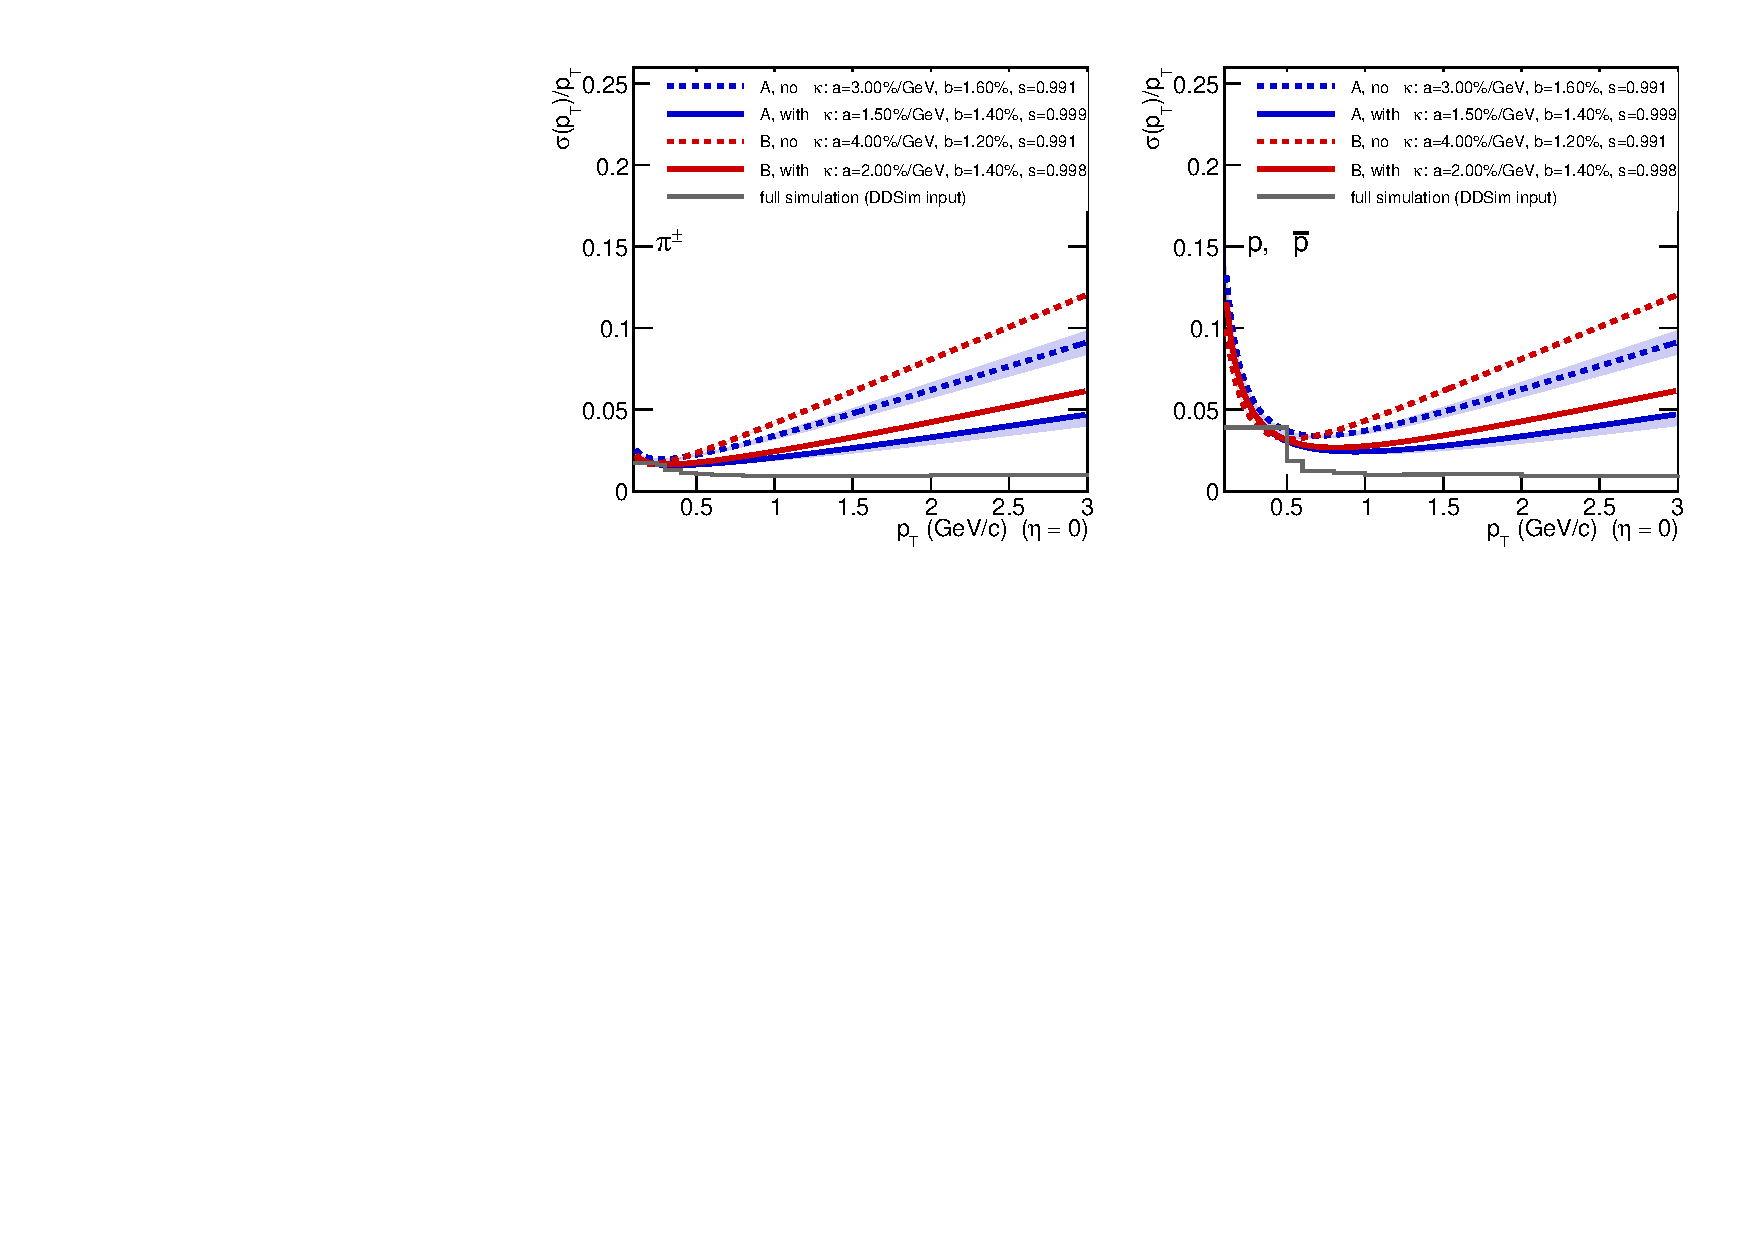
\includegraphics[width=\textwidth]{fig_res}
\caption{Fitted $\sigma(\pt)/\pt$ at $\eta=0$ (Eq.~\ref{eq:model}) for pions (left) and protons (right): period A (blue) and B
(red), without (dashed) and with (solid) $\kappa$; lines at the \Ks{} best point (Table~\ref{tab:summary}), bands = envelope of the $(a,b)$ grid nodes with
\Ks{} $\Delta\chi^2<2.3$ (profiled over $s$; \ResBandNote). Grey: full-simulation
response of the DDSim input. Script \fpath{scripts/plot_res.C}.}
\label{fig:res}
\end{figure}

For pions at 1, 2, 3\gevc: period A \PerARawResPiOne, \PerARawResPiTwo, \PerARawResPiThree\% without and \PerAKapResPiOne,
\PerAKapResPiTwo, \PerAKapResPiThree\% with $\kappa$; period B \PerBRawResPiOne, \PerBRawResPiTwo, \PerBRawResPiThree\% and
\PerBKapResPiOne, \PerBKapResPiTwo, \PerBKapResPiThree\%. Above $\approx1.5$\gevc{} the curves are constrained mainly by the two
highest \Ks{} bins (Table~\ref{tab:entries}).

\begin{figure}[H]
\centering
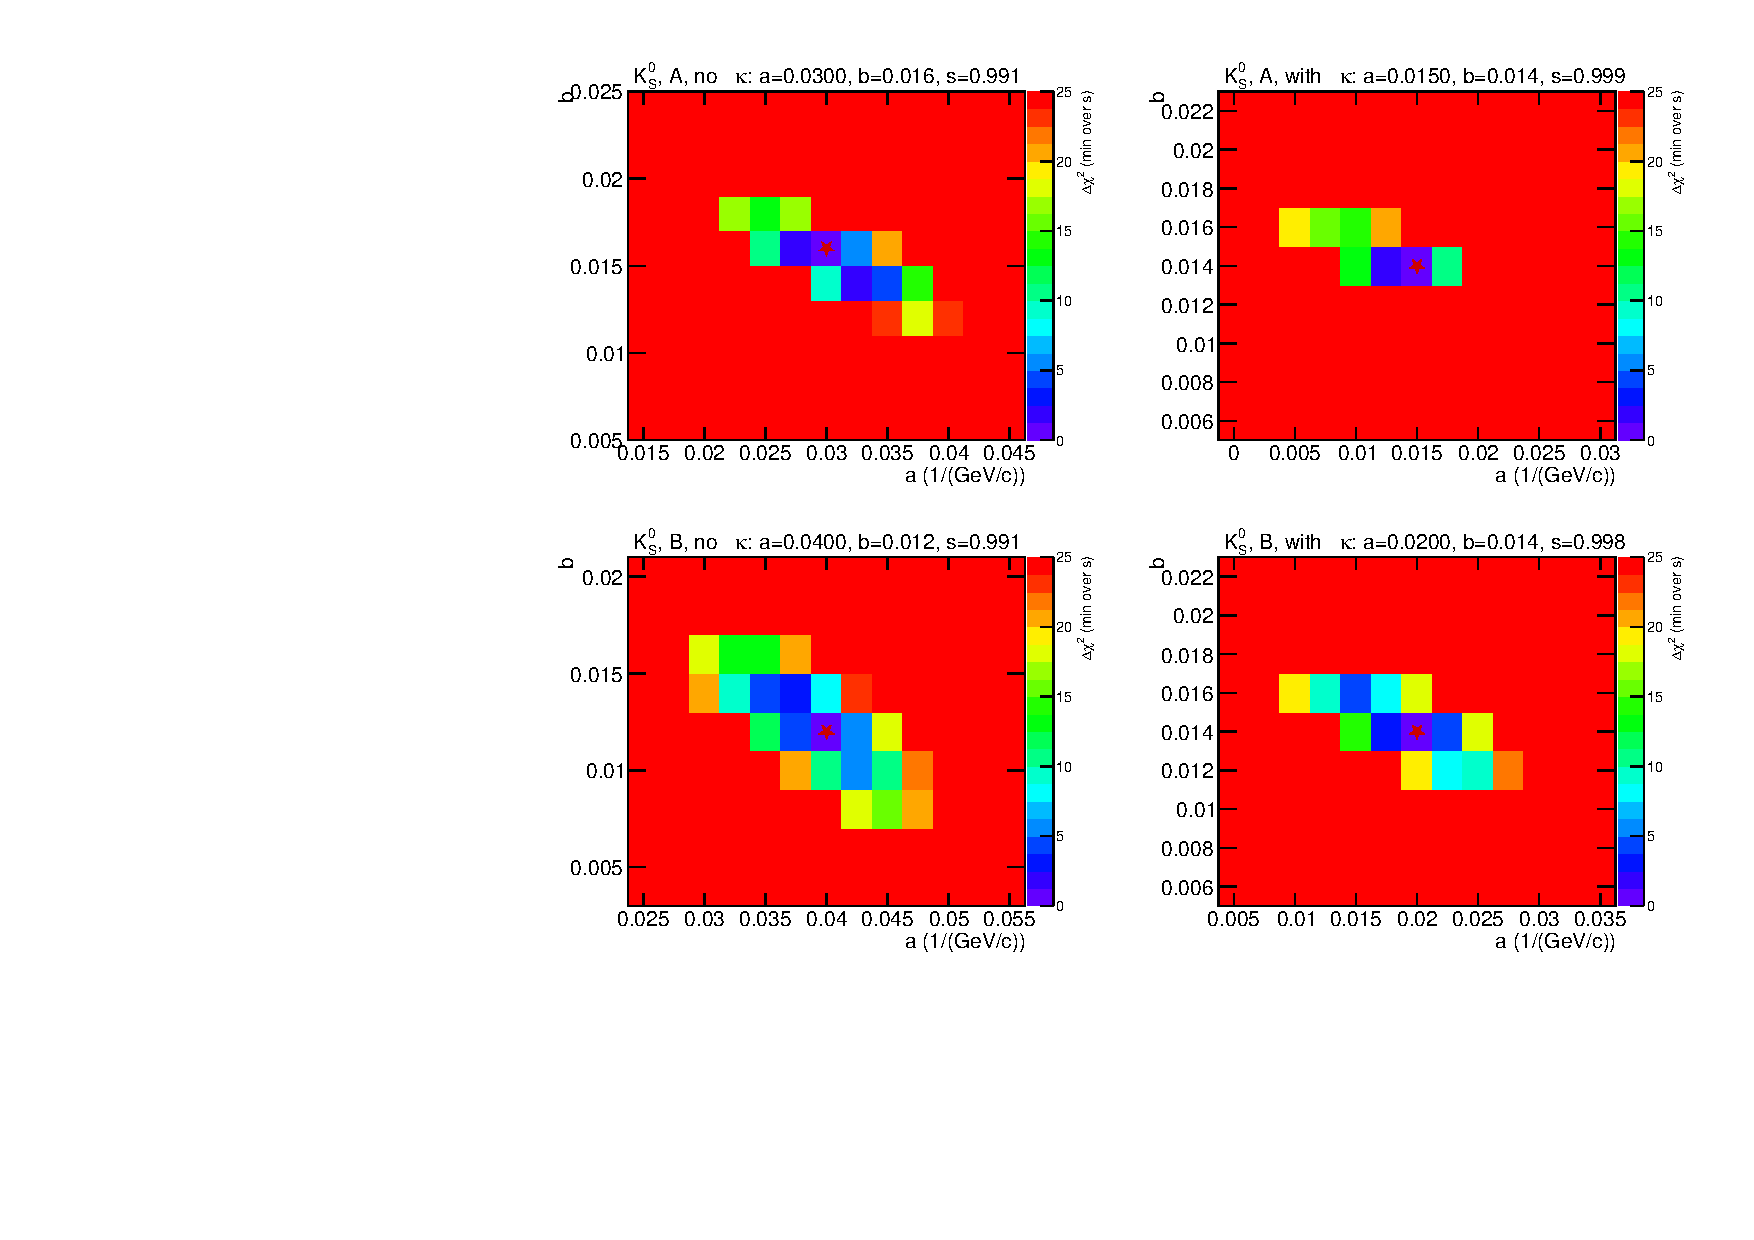
\includegraphics[width=0.92\textwidth]{fig_chi2}
\caption{$\Delta\chi^2$ of the \Ks{} fit in the $(a,b)$ plane, minimised over $s$, on the grid nodes (cells; colour scale
capped at 25): period A (top) and B (bottom), without (left) and with (right) $\kappa$. Red star: best node. The $\Delta\chi^2<2.3$ region is only a few nodes wide, so the
grid step (0.0025 in $a$, 0.002 in $b$) limits the resolution of the intervals. Each panel shows $\pm0.016$~(GeV/$c$)$^{-1}$ in $a$ and $\pm0.009$ in $b$ around its best node.}
\label{fig:chi2}
\end{figure}

\subsection{Invariant-mass distributions before and after the correction}
\label{sec:massdist}

Figure~\ref{fig:massdist} compares the \pt-integrated mass distributions of the same QA-selected candidates, recomputed from the
daughter momenta without $\kappa$ (blue) and with $\kappa$ (red); the KFParticle mass is shown for reference (grey). Only the
daughter \pt{} changes; $\eta$, $\varphi$ and the selection are the same. Figures~\ref{fig:massdistKsA}--\ref{fig:massdistLaB}
show the same per V0-\pt{} bin of the momentum fit (the V0 \pt{} is that of each version, so a candidate can change bin).

\begin{itemize}
\item \Ks: with $\kappa$ the peak moves up towards the PDG mass and becomes narrower and higher in both periods (Gaussian fit,
  Table~\ref{tab:peaksks}: mean \PerARawKsGM{} $\to$ \PerAKapKsGM, $\sigma$ \PerARawKsGS{} $\to$ \PerAKapKsGS\mevcc{} in A;
  \PerBRawKsGM{} $\to$ \PerBKapKsGM, \PerBRawKsGS{} $\to$ \PerBKapKsGS\mevcc{} in B). The change is largest above
  1.2\gevc, where the uncorrected peak is broad and the corrected one narrow.
\item \La: mean \PerARawLaGM{} $\to$ \PerAKapLaGM, $\sigma$ \PerARawLaGS{} $\to$ \PerAKapLaGS\mevcc{} (A) and
  \PerBRawLaGM{} $\to$ \PerBKapLaGM, \PerBRawLaGS{} $\to$ \PerBKapLaGS\mevcc{} (B), PDG \PdgLa\mevcc. The narrowing is smaller in
  absolute terms than for \Ks, as expected from the small \La{} decay momentum (the mass is less sensitive to the daughter momenta).
\item The background is the same in both recomputed versions. The number of entries in the plotted mass range differs by less than 1\%
  between them (\Ks{} A \PerAKsMdRaw{} vs \PerAKsMdKap, B \PerBKsMdRaw{} vs \PerBKsMdKap), as expected since the correction
  only moves masses by a few \mevcc.
\item The KFParticle mass has more combinatorial background in the same mass window (the recomputed spectra contain
  \PerAKsMdRatio{} (A) and \PerBKsMdRatio{} (B) of the KFP \Ks{} entries, \PerALaMdRatio{} and \PerBLaMdRatio{} for \La{}),
  although the candidates are the same. The cause is not investigated (open issue~3).
\end{itemize}

\begin{figure}[H]
\centering
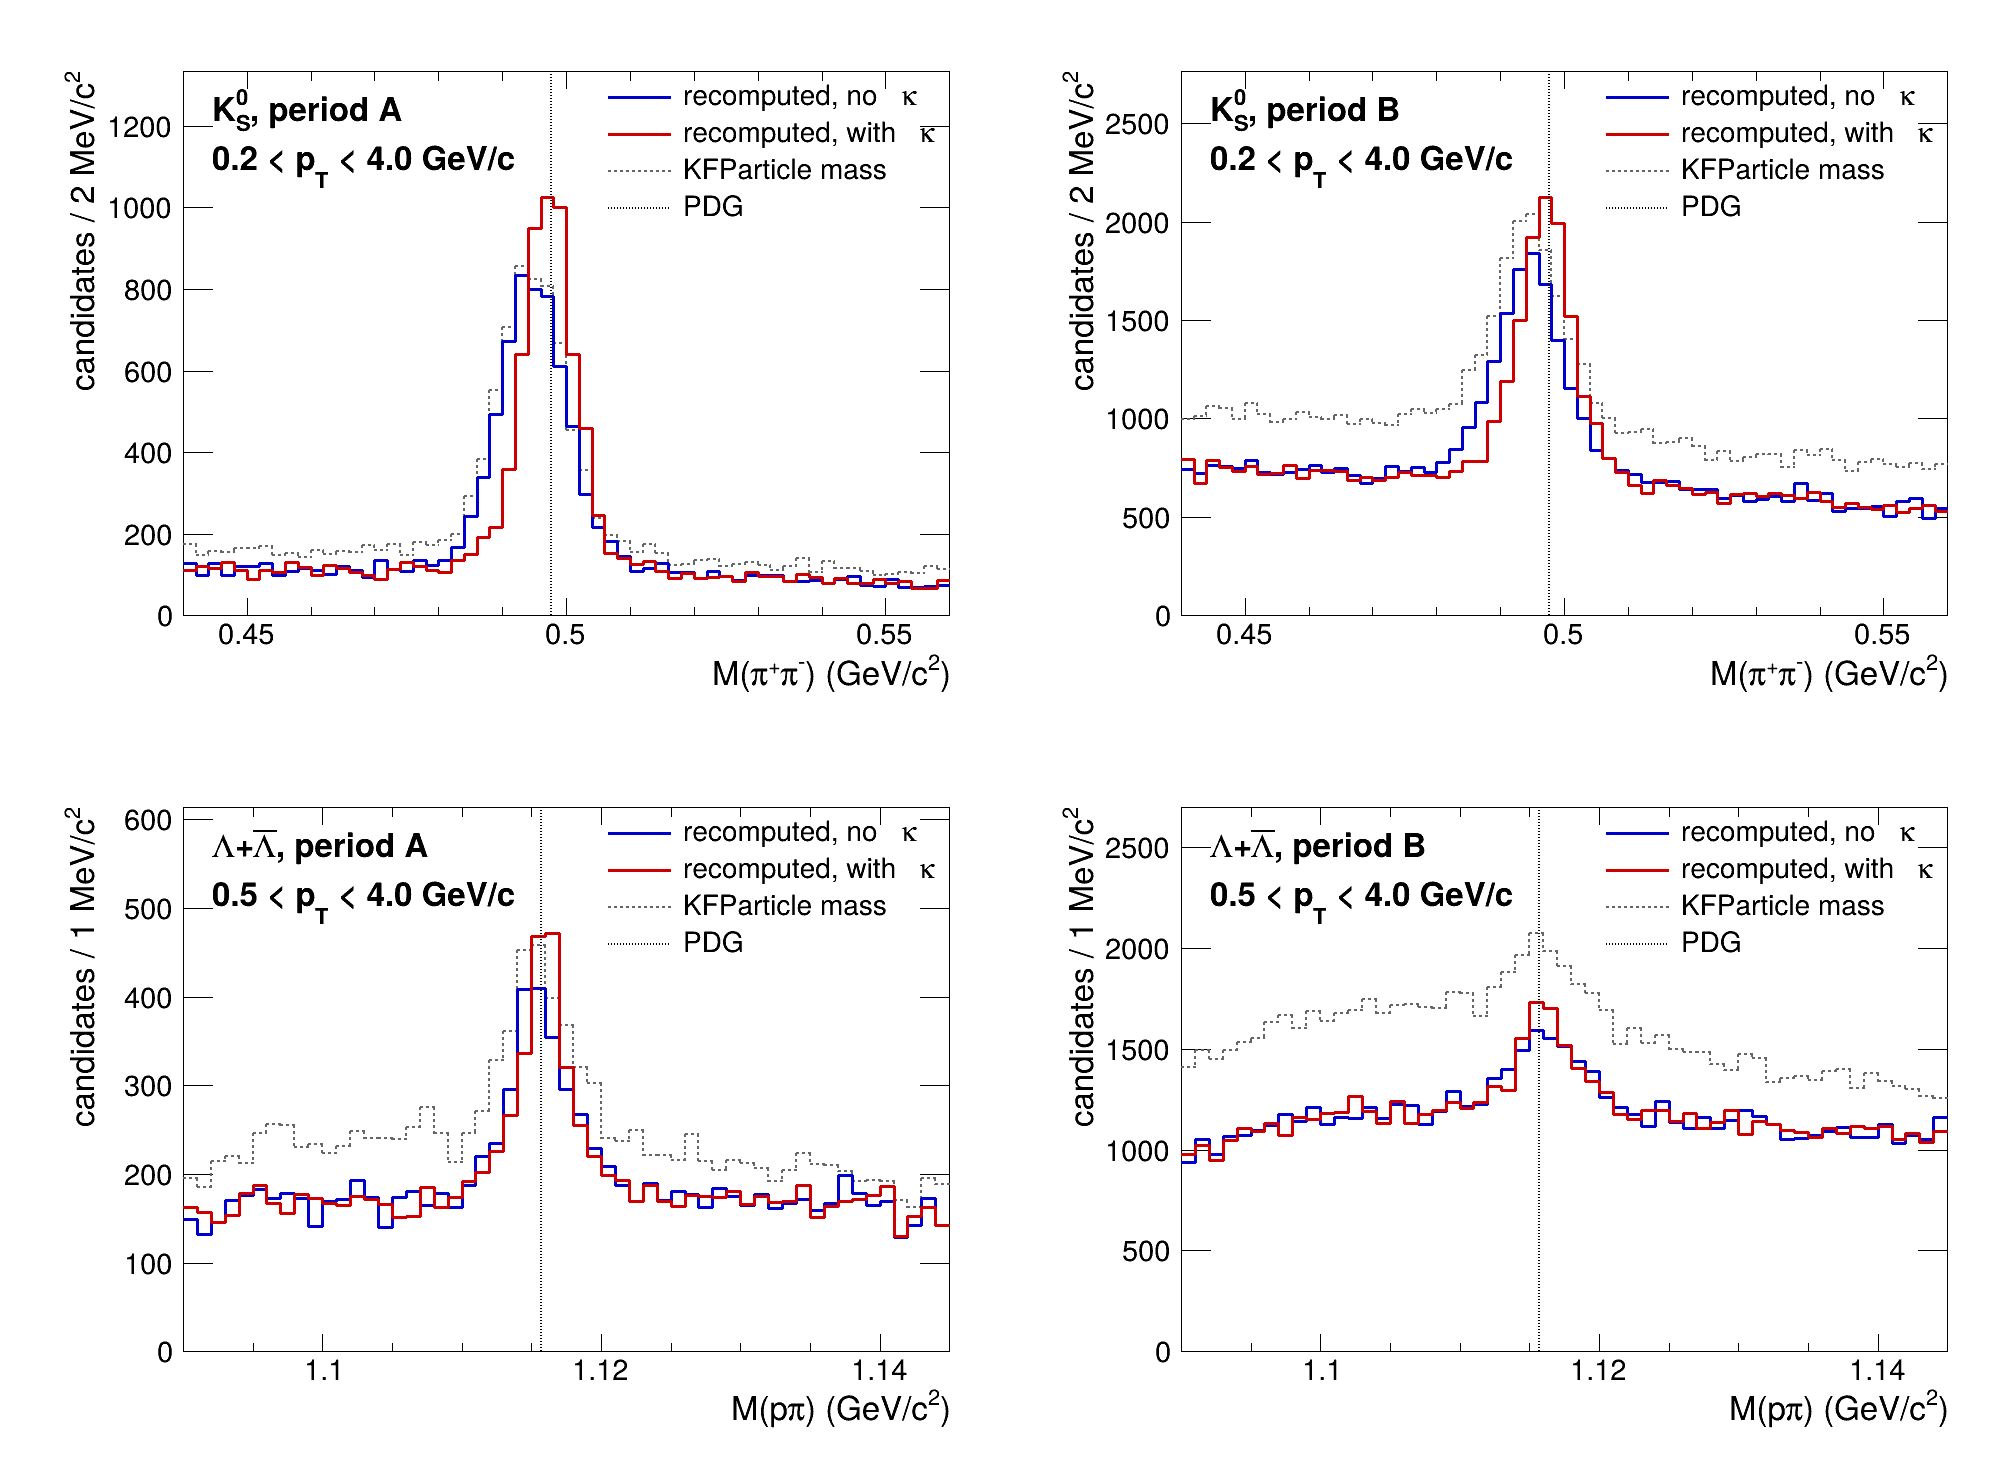
\includegraphics[width=\textwidth]{fig_massdist_int}
\caption{Invariant-mass distributions, \pt-integrated (\Ks{} $0.2<\pt<4.0$, \La+$\bar\Lambda$ $0.5<\pt<4.0$\gevc), period A
(left) and B (right): recomputed without $\kappa$ (blue), with $\kappa$ (red), KFParticle mass (grey dashed); dotted line: PDG
mass. Same QA-selected candidates in all curves. Script \fpath{scripts/massdist.C}.}
\label{fig:massdist}
\end{figure}

\begin{figure}[H]
\centering
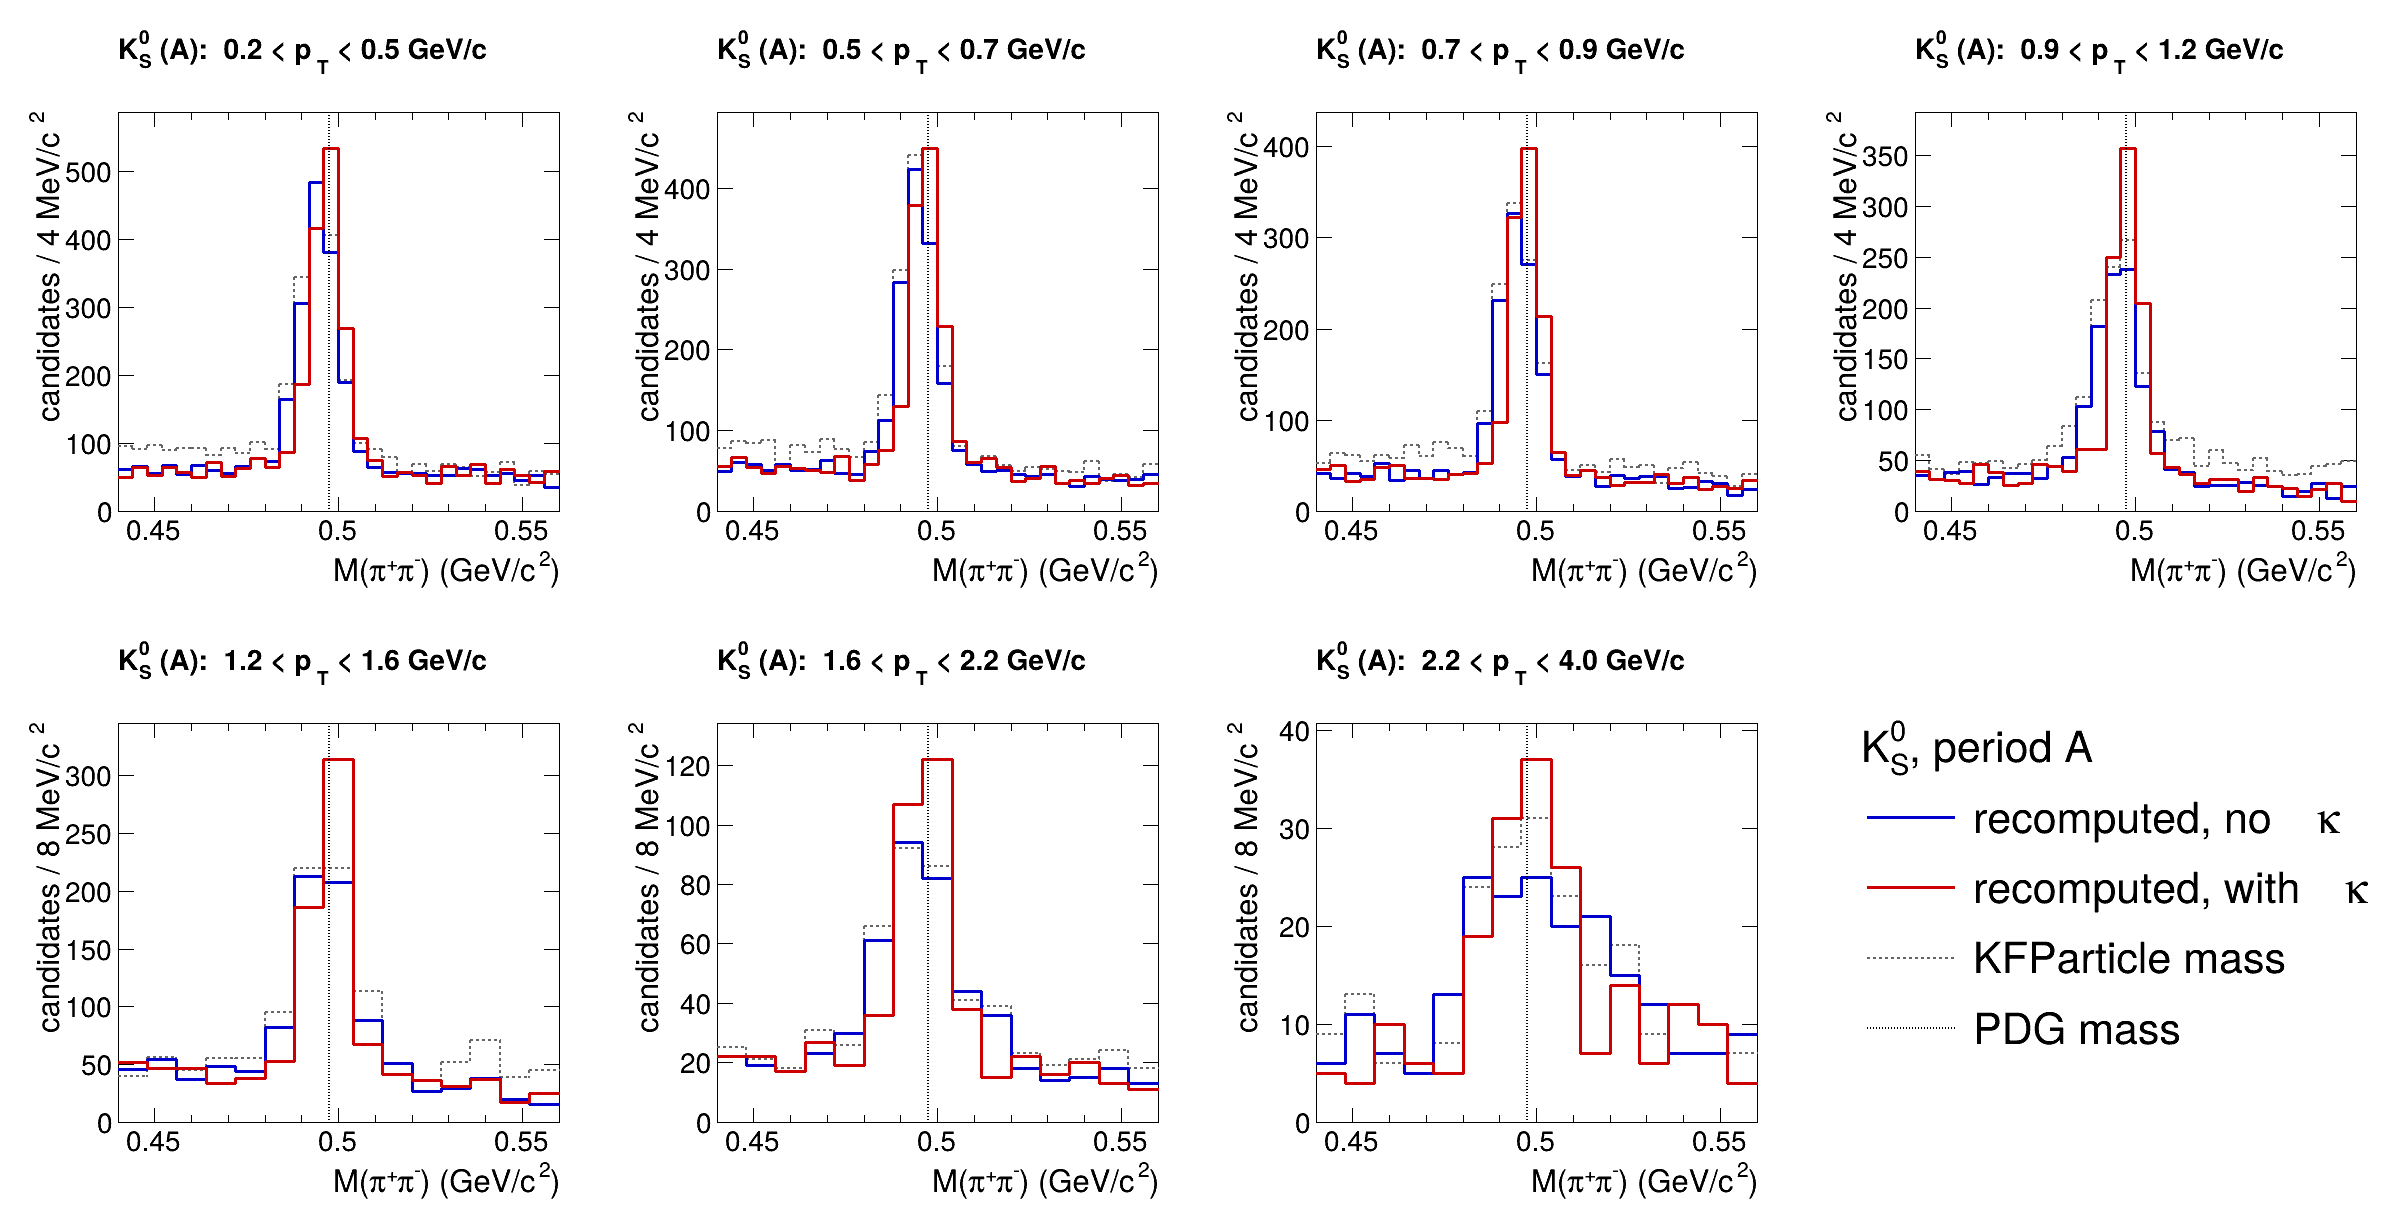
\includegraphics[width=\textwidth]{fig_massdist_Ks_A}
\caption{\Ks{} mass per V0-\pt{} bin, period A, without (blue) and with (red) $\kappa$, KFParticle mass (grey dashed). Bin width
2, 4 or 8\mevcc{} depending on the statistics of the panel (axis title).}
\label{fig:massdistKsA}
\end{figure}

\begin{figure}[H]
\centering
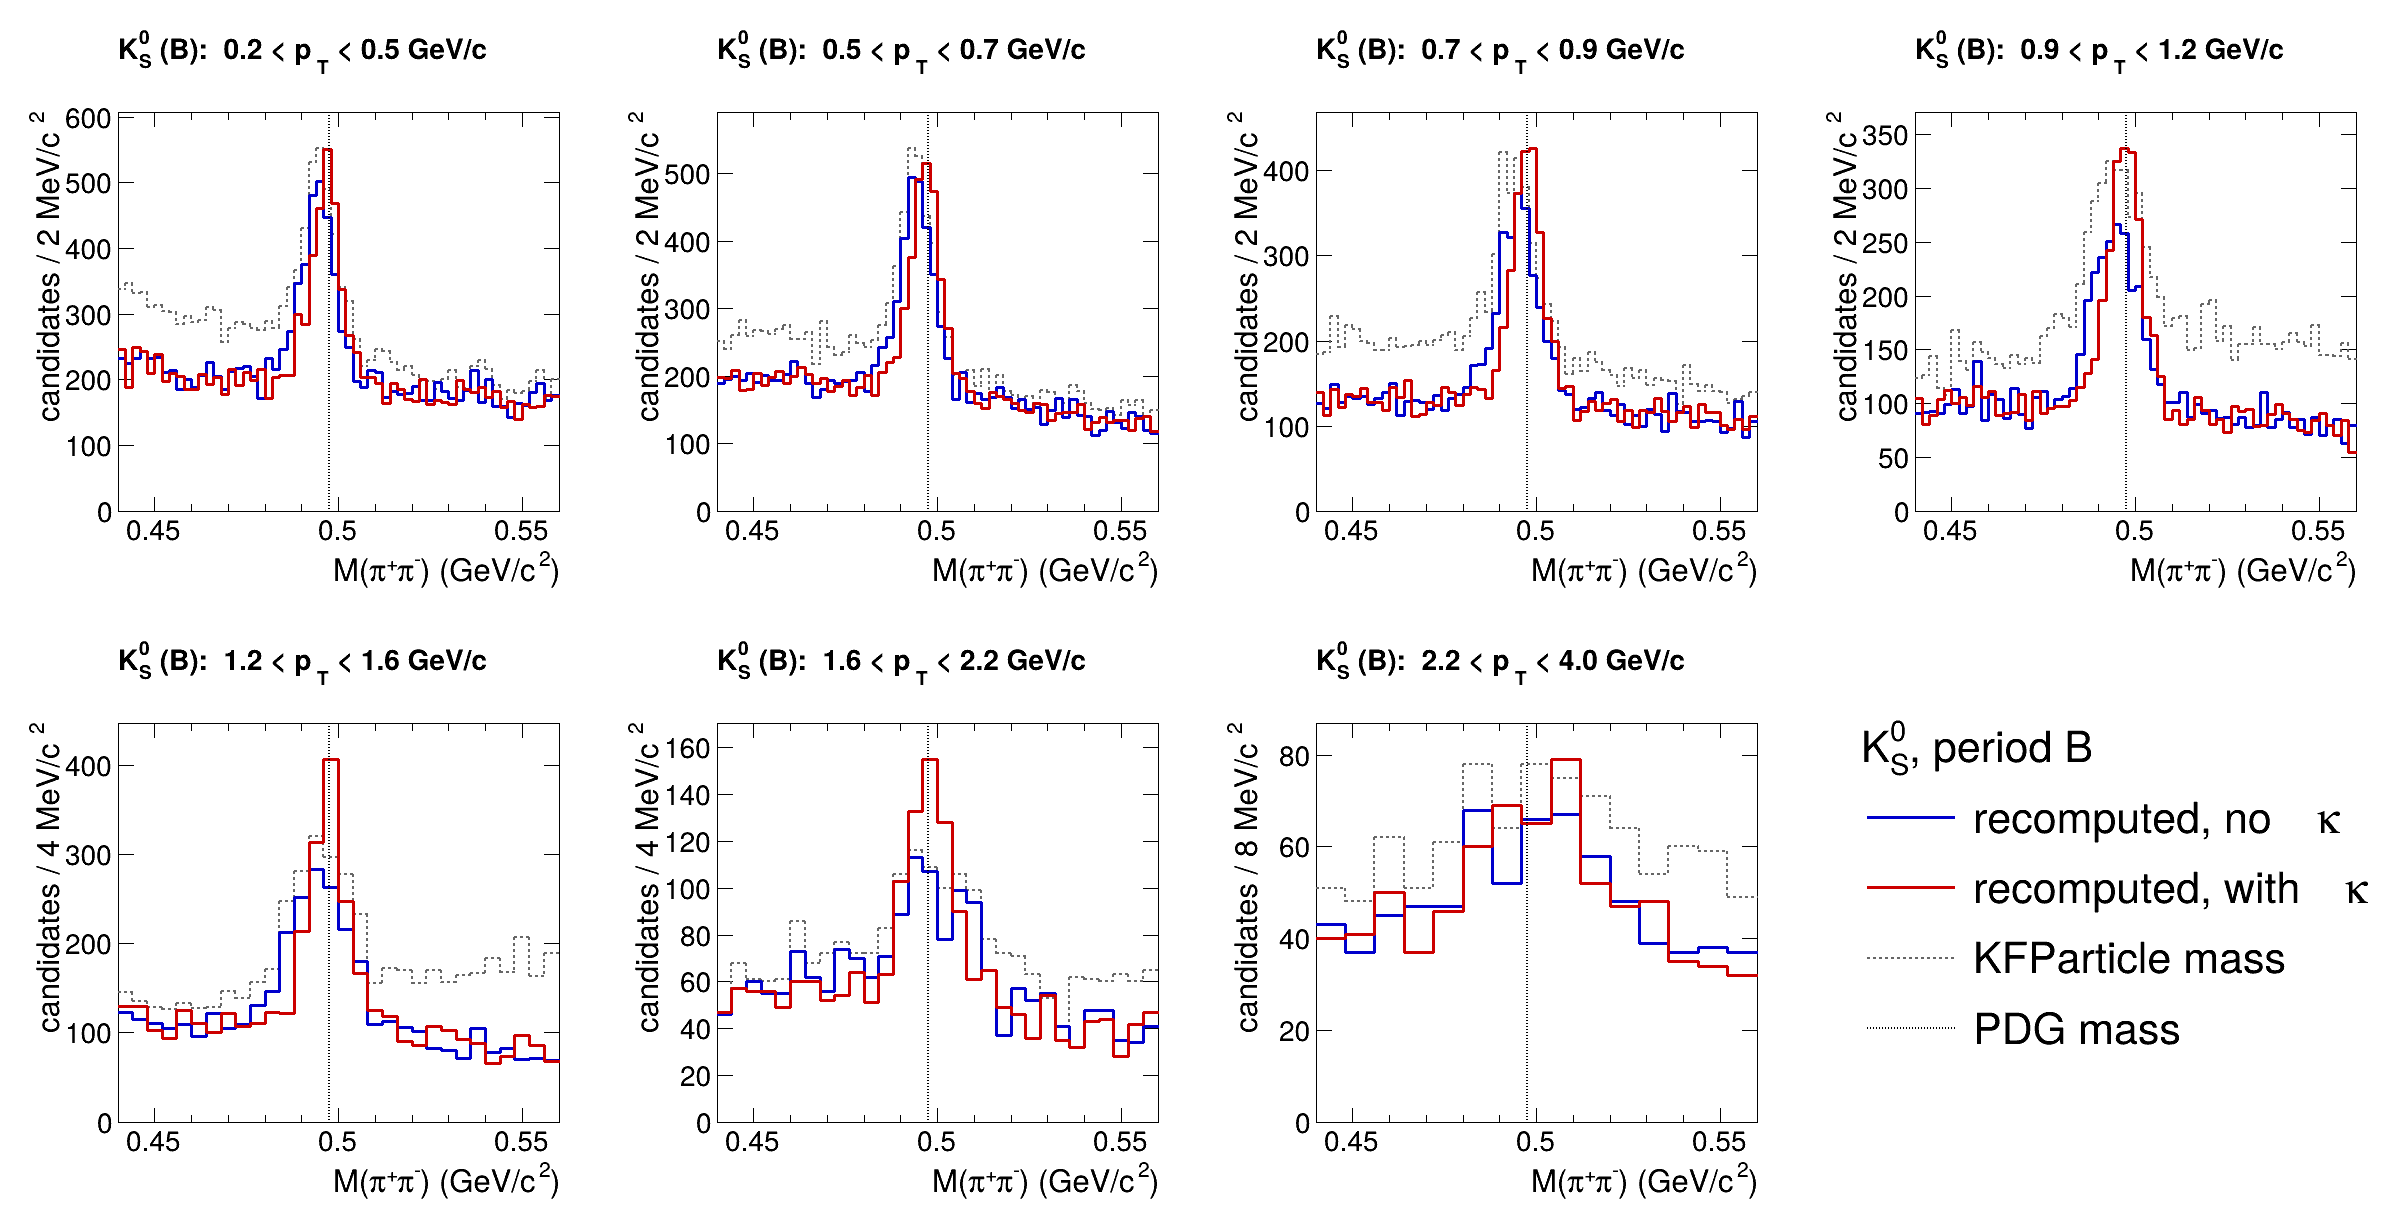
\includegraphics[width=\textwidth]{fig_massdist_Ks_B}
\caption{As Fig.~\ref{fig:massdistKsA}, period B.}
\label{fig:massdistKsB}
\end{figure}

\begin{figure}[H]
\centering
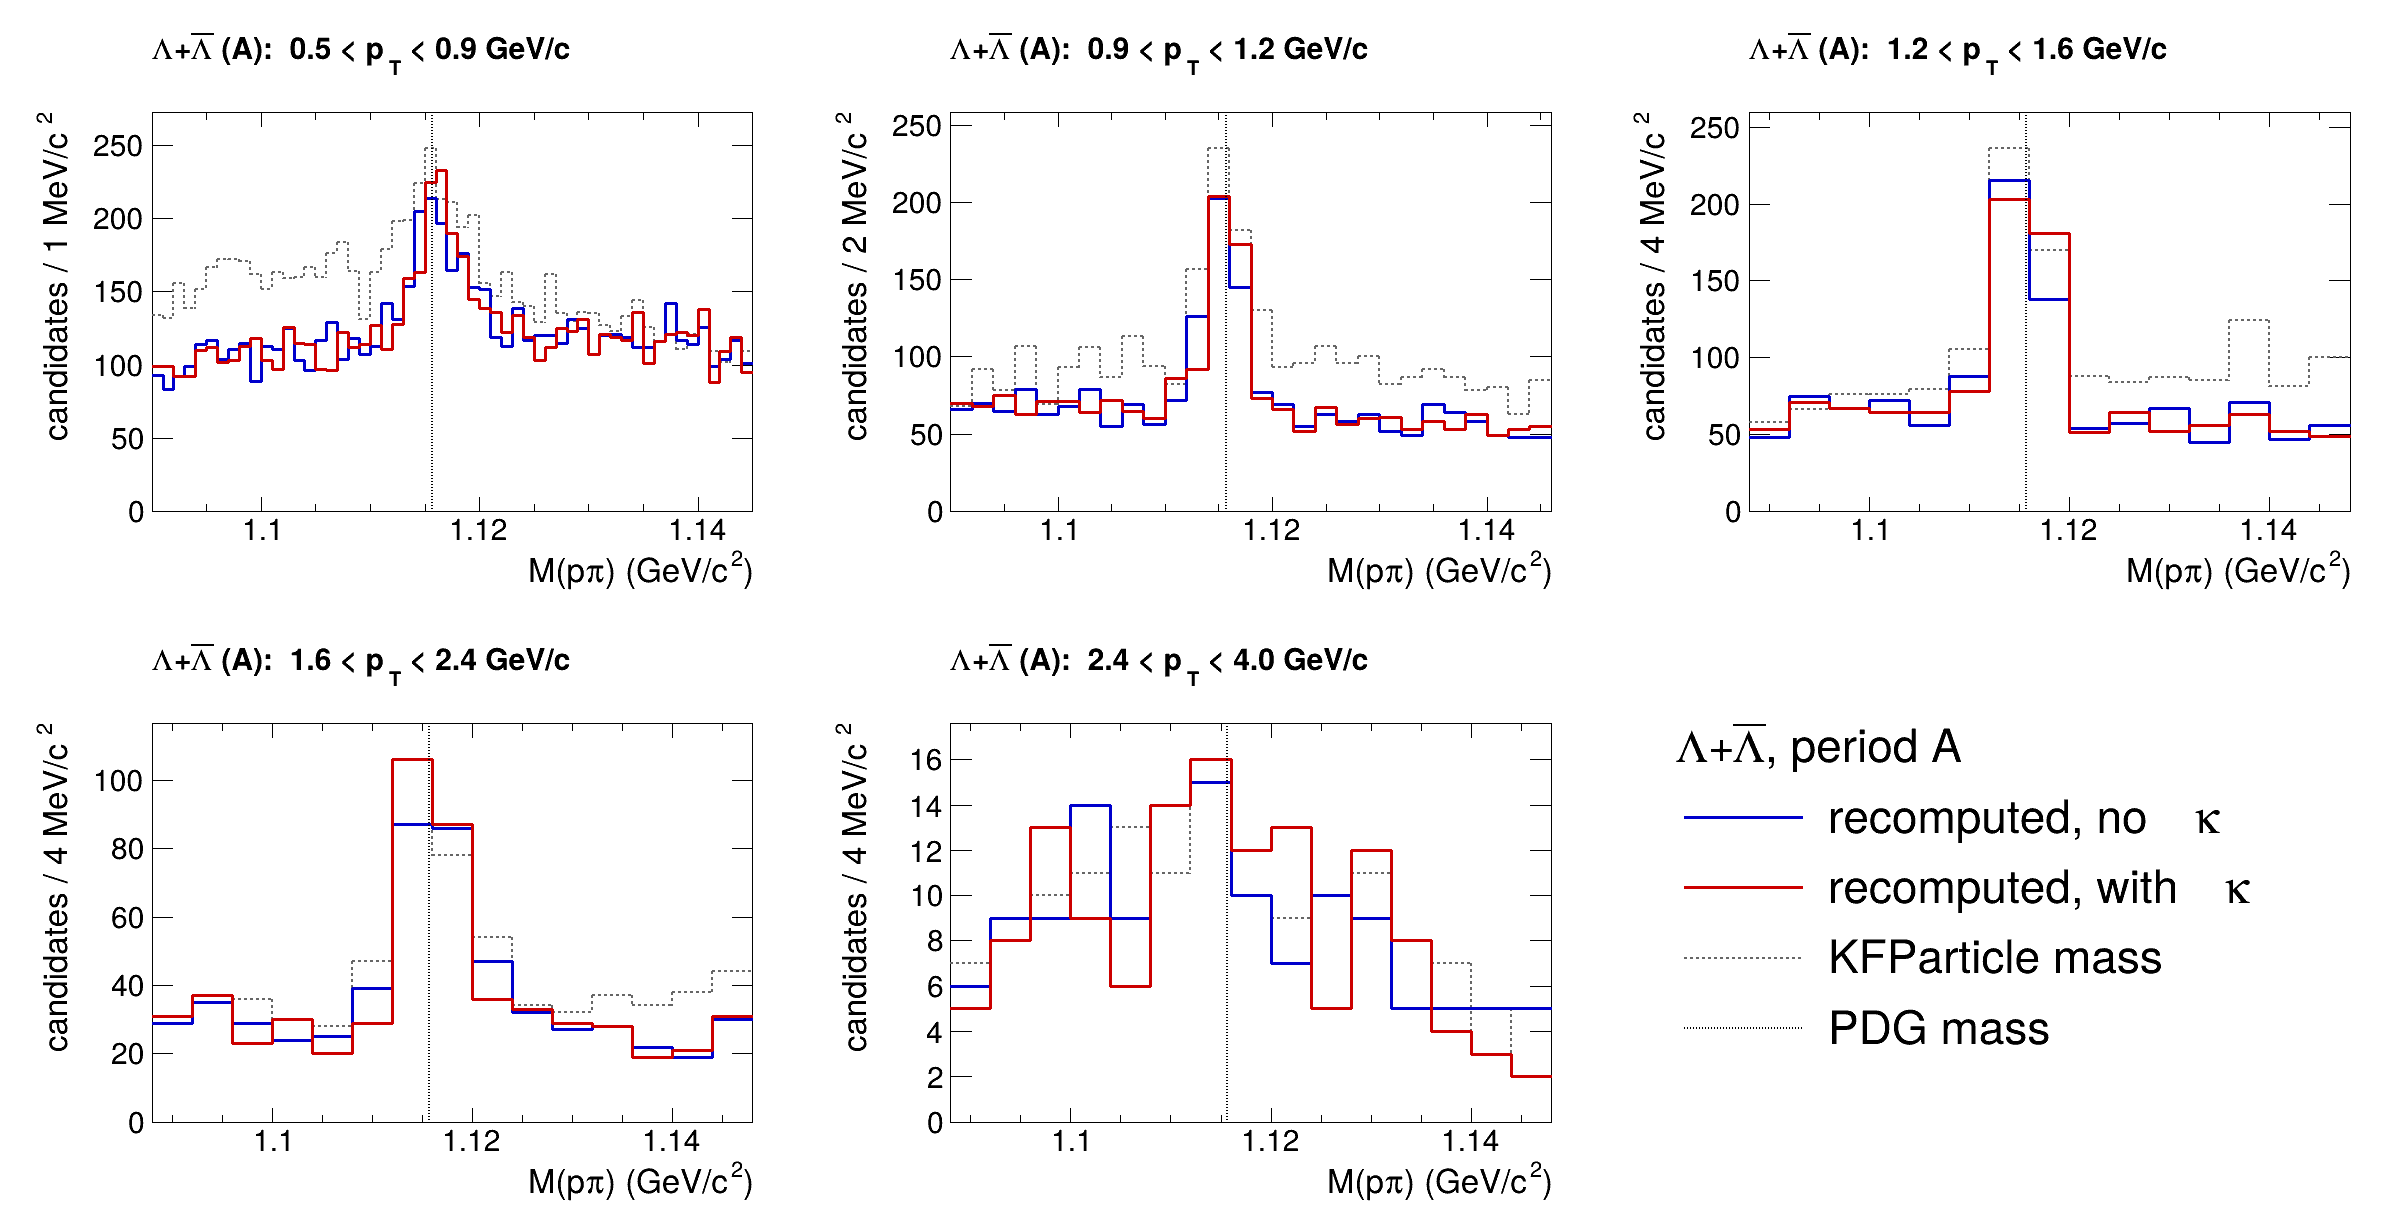
\includegraphics[width=\textwidth]{fig_massdist_La_A}
\caption{\La+$\bar\Lambda$ mass per V0-\pt{} bin, period A, without (blue) and with (red) $\kappa$, KFParticle mass (grey dashed).
Bin width 1, 2 or 4\mevcc{} depending on the statistics of the panel.}
\label{fig:massdistLaA}
\end{figure}

\begin{figure}[H]
\centering
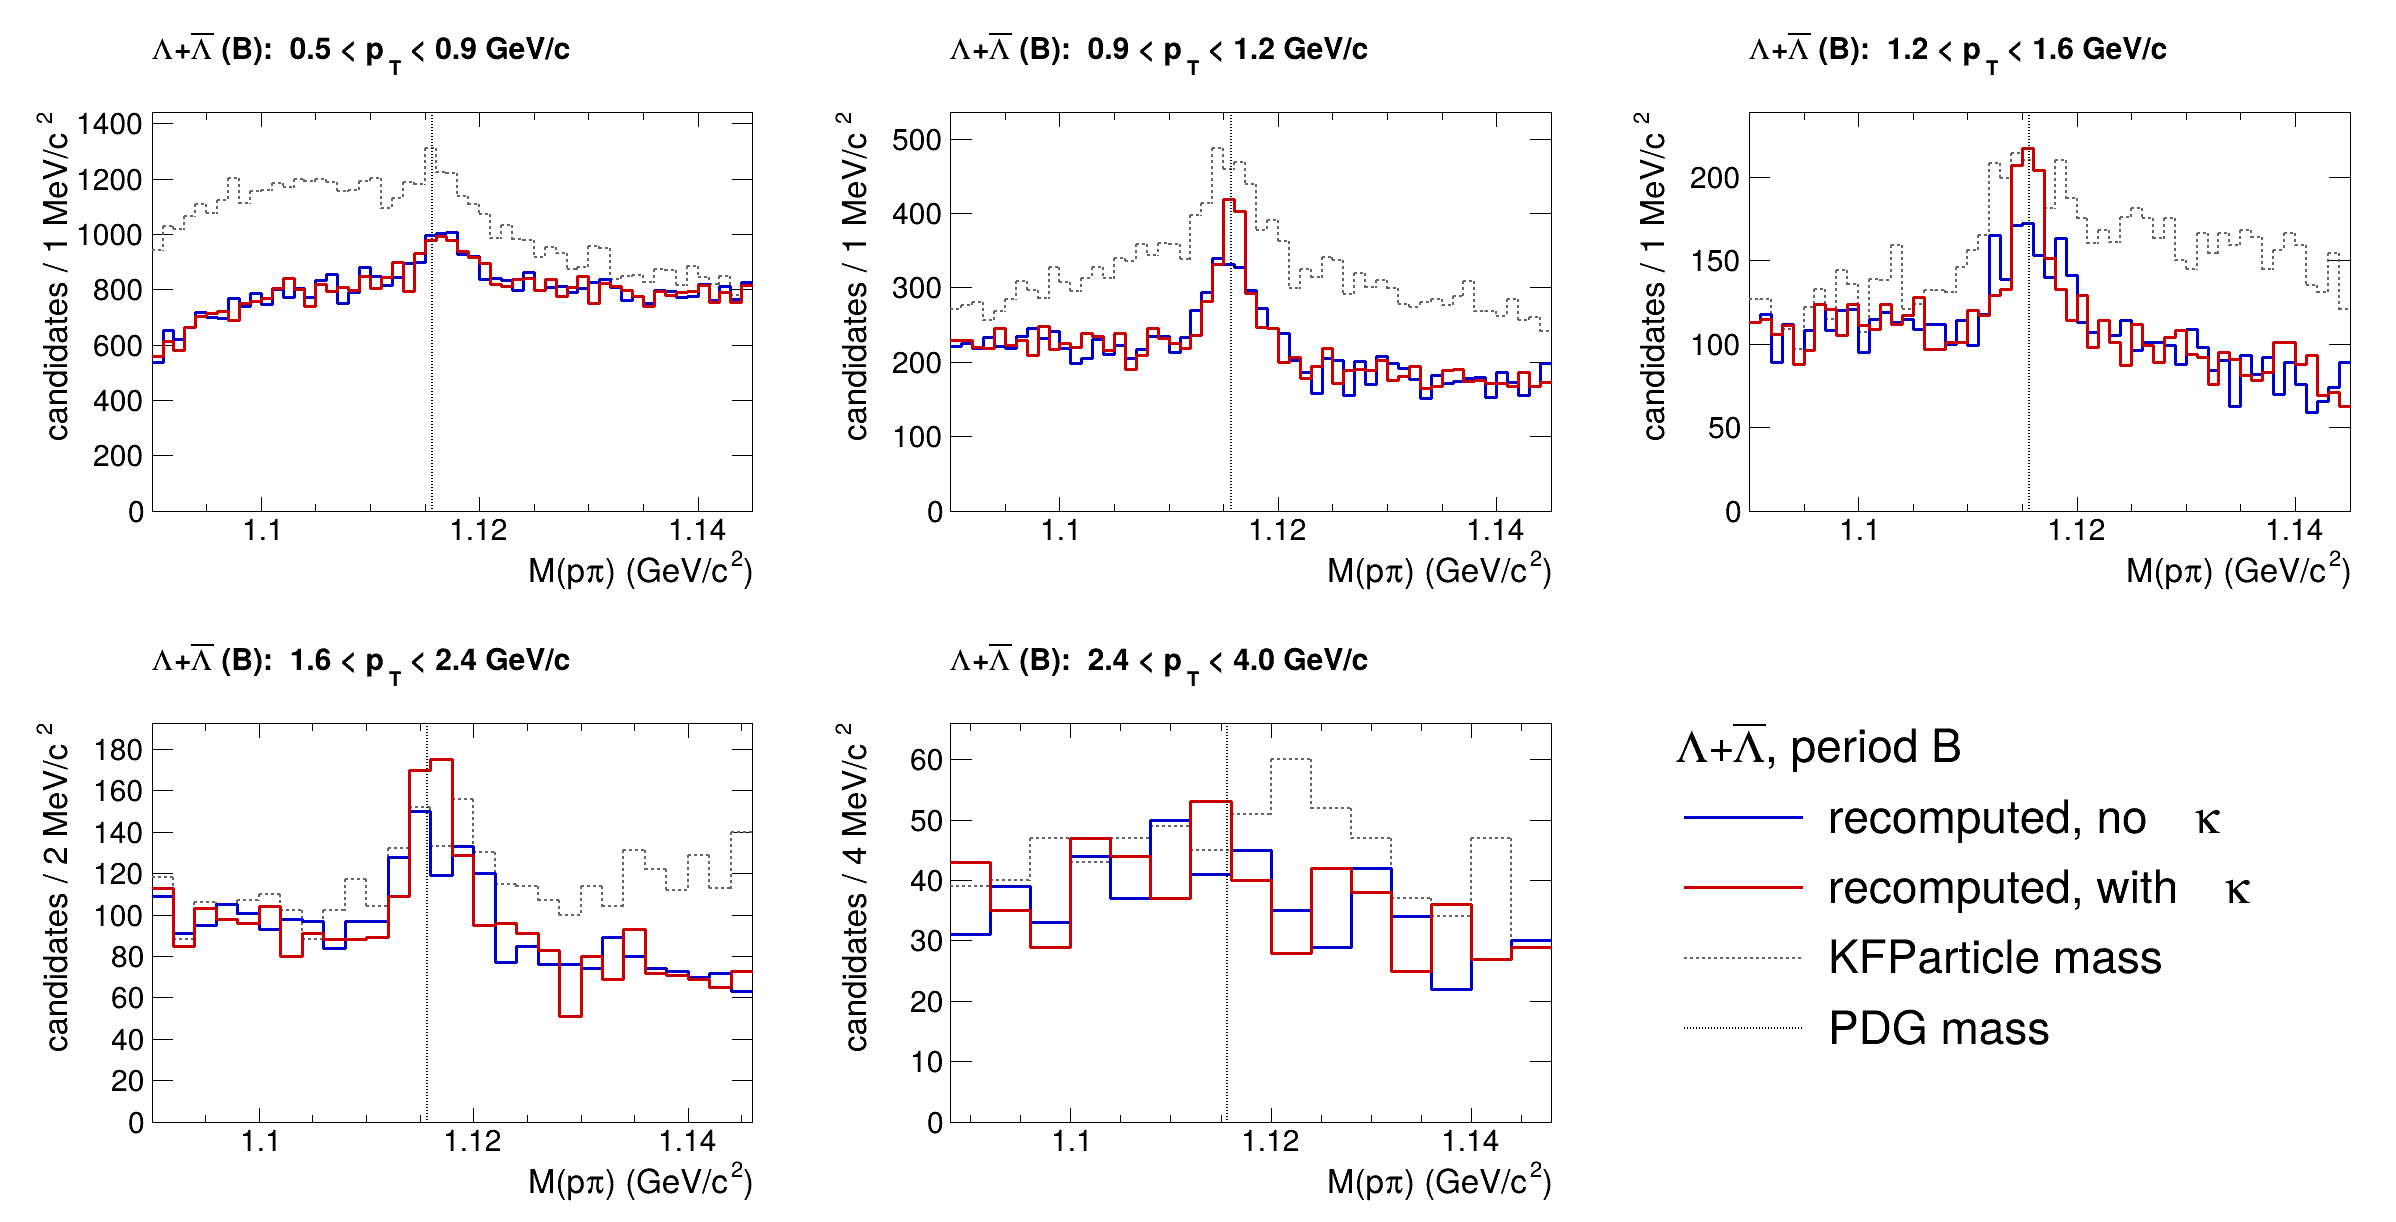
\includegraphics[width=\textwidth]{fig_massdist_La_B}
\caption{As Fig.~\ref{fig:massdistLaA}, period B.}
\label{fig:massdistLaB}
\end{figure}

\subsection{Mass peaks}

\begin{figure}[H]
\centering
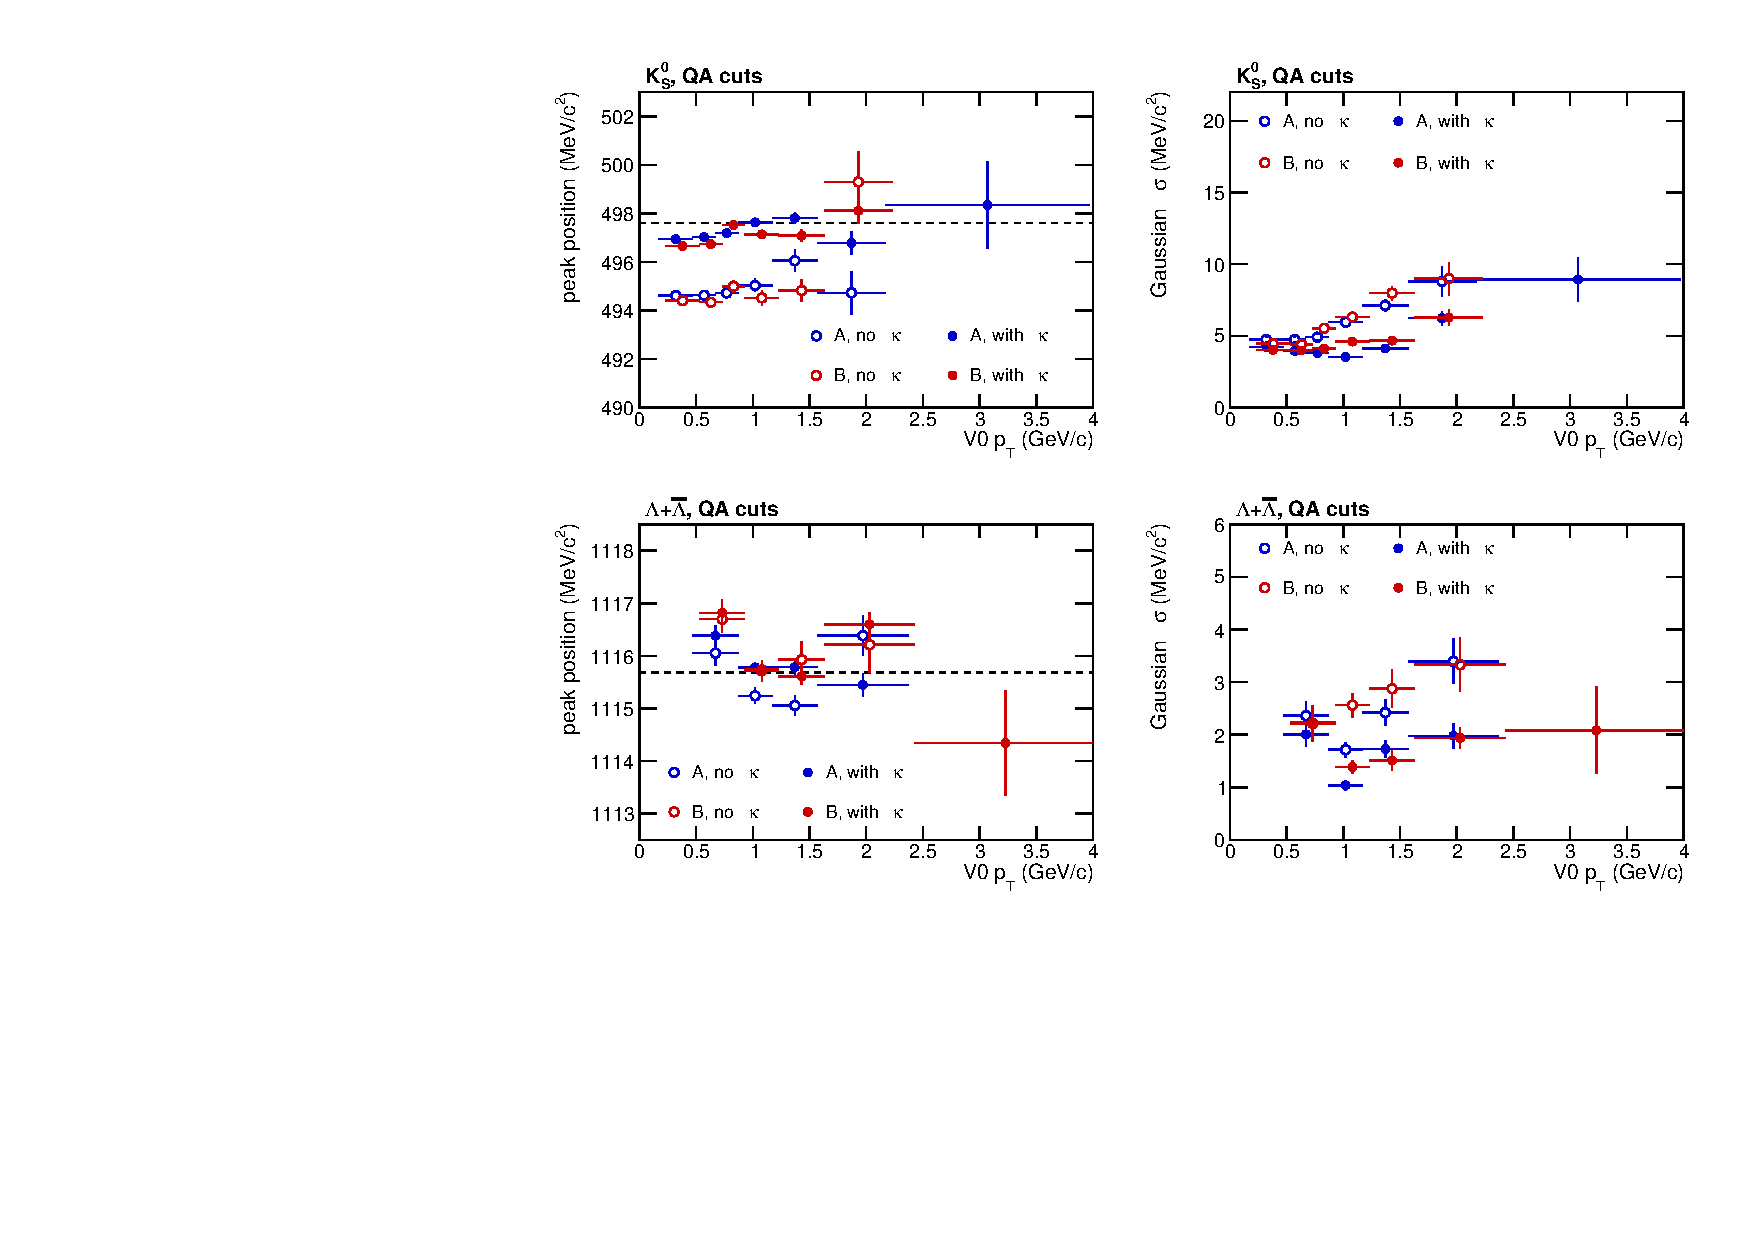
\includegraphics[width=\textwidth]{fig_peaks}
\caption{Gaussian peak position (left) and width (right) per V0-\pt{} bin for \Ks{} (top; Gaussian + linear, 0.46--0.54~GeV/$c^2$)
and \La+$\bar\Lambda$ (bottom; Gaussian + quadratic, 1.103--1.130~GeV/$c^2$): period A (blue) and B (red), without (open) and
with (full) $\kappa$; points of the two periods are offset by $\pm0.03$\gevc{} for visibility. Dashed: PDG mass. Unconstrained fits
(mean error $>2$\mevcc{} or width error $>60\%$) are not drawn. Display only; the calibration uses the template fit.
Script \fpath{scripts/peaks.C}.}
\label{fig:peaks}
\end{figure}

\begin{table}[H]
\centering\footnotesize
\caption{\Ks{} Gaussian peak position $M$ and width $\sigma$ (MeV/$c^2$) per V0-\pt{} bin (GeV/$c$), fits of
Fig.~\ref{fig:peaks}; ``--'' unconstrained. PDG \PdgKs\mevcc.}
\label{tab:peaksks}
\setlength{\tabcolsep}{2.4pt}
\begin{tabular}{lcccccccc}
\toprule
 & \multicolumn{4}{c}{period A} & \multicolumn{4}{c}{period B} \\
\pt & $M$, no $\kappa$ & $\sigma$, no $\kappa$ & $M$, $\kappa$ & $\sigma$, $\kappa$ & $M$, no $\kappa$ & $\sigma$, no $\kappa$ & $M$, $\kappa$ & $\sigma$, $\kappa$ \\
\midrule
% generated by scripts/make_numbers.py
0.2--0.5 & 494.61$\pm$0.17 & 4.74$\pm$0.16 & 496.94$\pm$0.15 & 4.23$\pm$0.15 & 494.41$\pm$0.20 & 4.46$\pm$0.22 & 496.65$\pm$0.18 & 4.02$\pm$0.20 \\
0.5--0.7 & 494.63$\pm$0.18 & 4.75$\pm$0.17 & 497.02$\pm$0.15 & 3.96$\pm$0.15 & 494.34$\pm$0.19 & 4.42$\pm$0.20 & 496.73$\pm$0.16 & 3.98$\pm$0.17 \\
0.7--0.9 & 494.72$\pm$0.20 & 4.91$\pm$0.18 & 497.19$\pm$0.15 & 3.80$\pm$0.13 & 494.99$\pm$0.24 & 5.53$\pm$0.27 & 497.53$\pm$0.17 & 4.11$\pm$0.17 \\
0.9--1.2 & 495.03$\pm$0.27 & 5.95$\pm$0.27 & 497.64$\pm$0.15 & 3.53$\pm$0.14 & 494.52$\pm$0.30 & 6.32$\pm$0.30 & 497.14$\pm$0.19 & 4.60$\pm$0.19 \\
1.2--1.6 & 496.05$\pm$0.45 & 7.12$\pm$0.39 & 497.81$\pm$0.23 & 4.12$\pm$0.23 & 494.82$\pm$0.46 & 7.99$\pm$0.49 & 497.09$\pm$0.25 & 4.67$\pm$0.28 \\
1.6--2.2 & 494.73$\pm$0.89 & 8.79$\pm$1.03 & 496.79$\pm$0.48 & 6.24$\pm$0.48 & 499.30$\pm$1.25 & 9.00$\pm$1.15 & 498.11$\pm$0.51 & 6.27$\pm$0.56 \\
2.2--4.0 & -- & -- & 498.34$\pm$1.78 & 8.92$\pm$1.55 & -- & -- & -- & -- \\
0.2--4.0 (all) & 494.78$\pm$0.10 & 5.30$\pm$0.10 & 497.21$\pm$0.07 & 4.03$\pm$0.07 & 494.57$\pm$0.11 & 5.43$\pm$0.13 & 497.04$\pm$0.08 & 4.33$\pm$0.09 \\

\bottomrule
\end{tabular}
\end{table}

\begin{table}[H]
\centering\footnotesize
\caption{As Table~\ref{tab:peaksks} for \La+$\bar\Lambda$. PDG \PdgLa\mevcc.}
\label{tab:peaksla}
\setlength{\tabcolsep}{2.4pt}
\begin{tabular}{lcccccccc}
\toprule
 & \multicolumn{4}{c}{period A} & \multicolumn{4}{c}{period B} \\
\pt & $M$, no $\kappa$ & $\sigma$, no $\kappa$ & $M$, $\kappa$ & $\sigma$, $\kappa$ & $M$, no $\kappa$ & $\sigma$, no $\kappa$ & $M$, $\kappa$ & $\sigma$, $\kappa$ \\
\midrule
% generated by scripts/make_numbers.py
0.5--0.9 & 1116.05$\pm$0.24 & 2.36$\pm$0.28 & 1116.38$\pm$0.19 & 2.01$\pm$0.24 & 1116.70$\pm$0.26 & 2.21$\pm$0.35 & 1116.82$\pm$0.25 & 2.24$\pm$0.32 \\
0.9--1.2 & 1115.24$\pm$0.15 & 1.72$\pm$0.14 & 1115.78$\pm$0.10 & 1.04$\pm$0.09 & 1115.72$\pm$0.20 & 2.56$\pm$0.23 & 1115.75$\pm$0.10 & 1.39$\pm$0.13 \\
1.2--1.6 & 1115.06$\pm$0.20 & 2.42$\pm$0.24 & 1115.79$\pm$0.14 & 1.73$\pm$0.17 & 1115.93$\pm$0.35 & 2.88$\pm$0.36 & 1115.61$\pm$0.15 & 1.51$\pm$0.18 \\
1.6--2.4 & 1116.39$\pm$0.38 & 3.40$\pm$0.43 & 1115.45$\pm$0.22 & 1.98$\pm$0.24 & 1116.21$\pm$0.52 & 3.33$\pm$0.51 & 1116.60$\pm$0.22 & 1.94$\pm$0.19 \\
2.4--4.0 & -- & -- & -- & -- & -- & -- & 1114.34$\pm$1.00 & 2.08$\pm$0.83 \\
0.5--4.0 (all) & 1115.55$\pm$0.12 & 2.16$\pm$0.14 & 1115.92$\pm$0.08 & 1.63$\pm$0.11 & 1116.24$\pm$0.16 & 2.69$\pm$0.19 & 1116.11$\pm$0.10 & 1.88$\pm$0.13 \\

\bottomrule
\end{tabular}
\end{table}

\subsection{Template fits per V0-\pt{} bin}

Figures~\ref{fig:massksA}--\ref{fig:masslaB} show the data with the template fit at the \Ks{} best point of the $\kappa$-corrected
fits (the \La{} panels are therefore a prediction from the \Ks{} parameters, not a \La{} fit). The uncorrected versions are in
Appendix~\ref{app:raw}. Per-bin $\chi^2$: Table~\ref{tab:binchi}.

\begin{figure}[H]
\centering
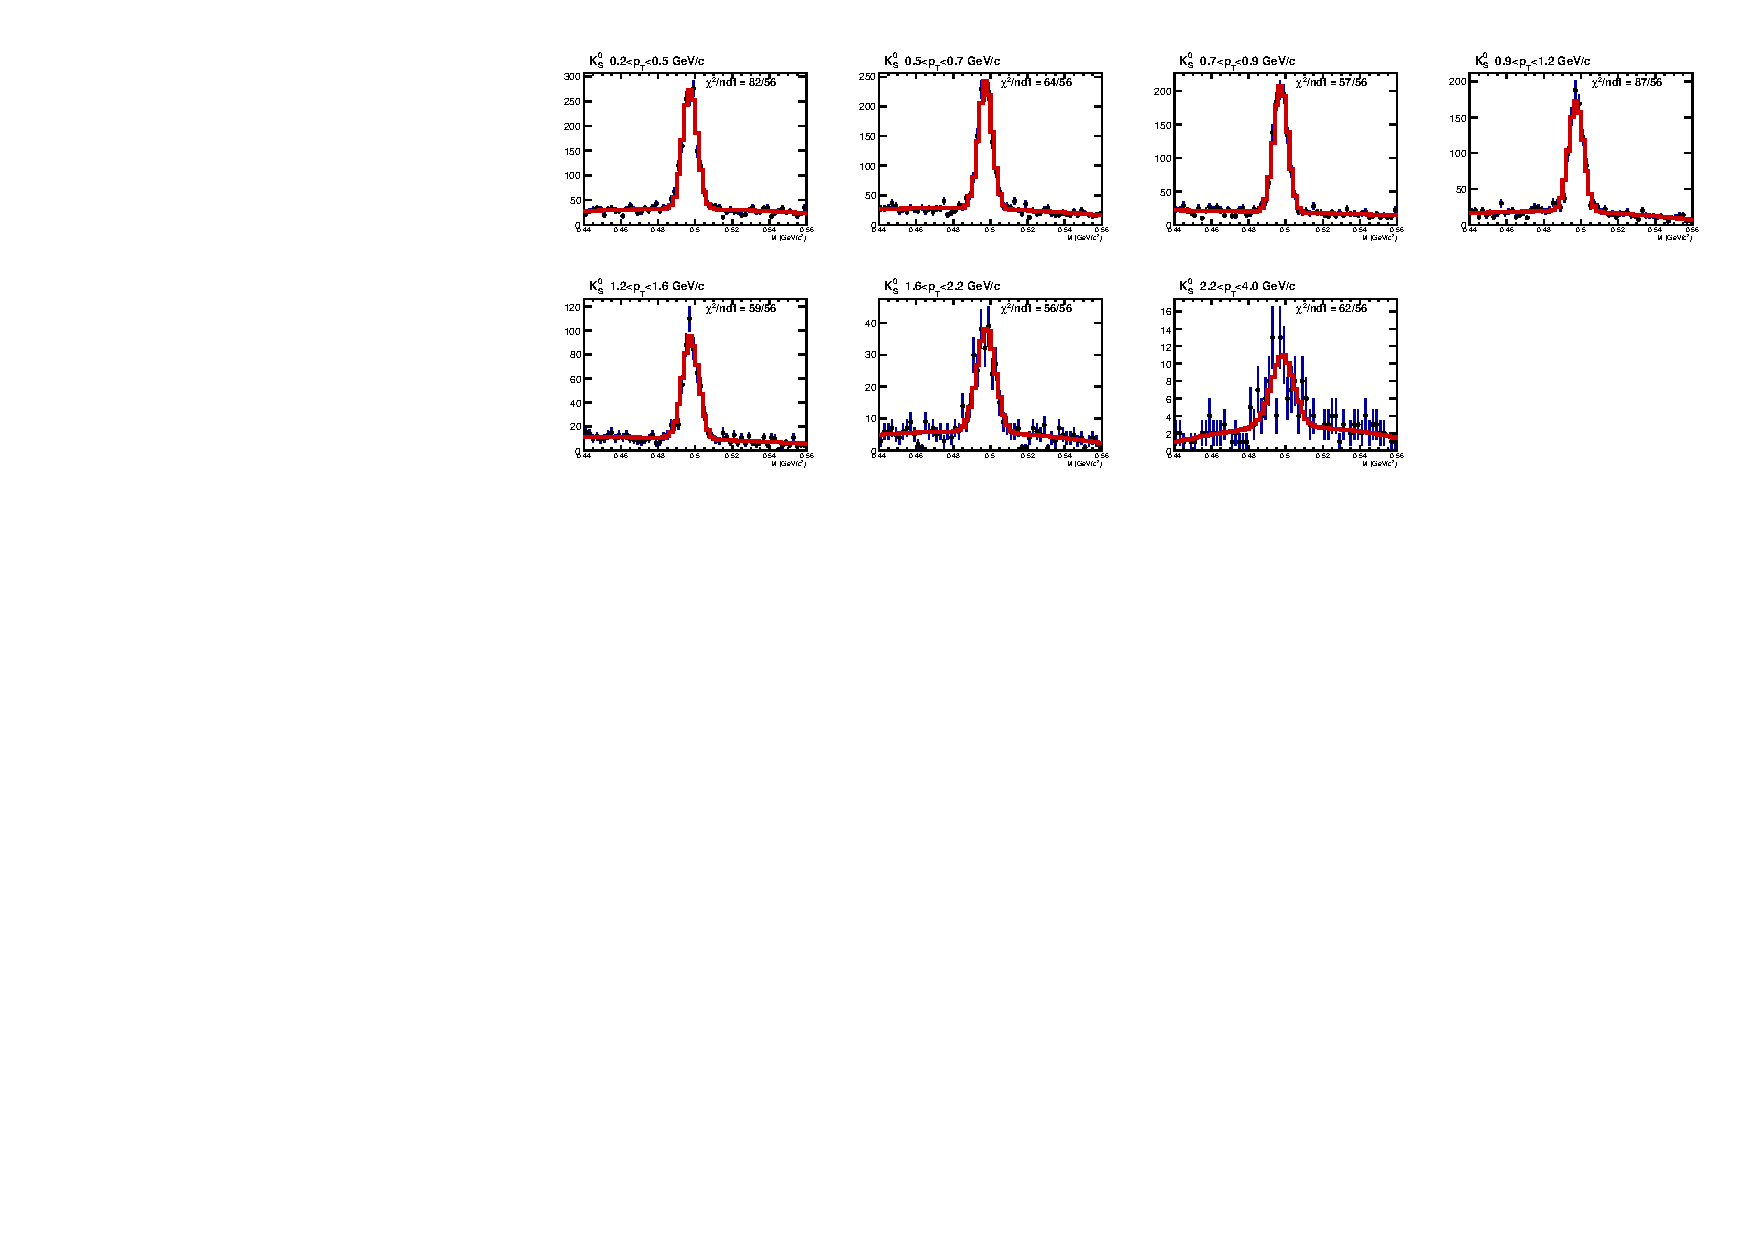
\includegraphics[width=\textwidth]{fig_mass_Ks_A_kappa}
\caption{\Ks{} mass per V0-\pt{} bin, period A, with $\kappa$ (points), and $N\times$DDSim template + quadratic background at the
\Ks{} best point (red); per-panel Baker--Cousins $\chi^2$/ndf.}
\label{fig:massksA}
\end{figure}

\begin{figure}[H]
\centering
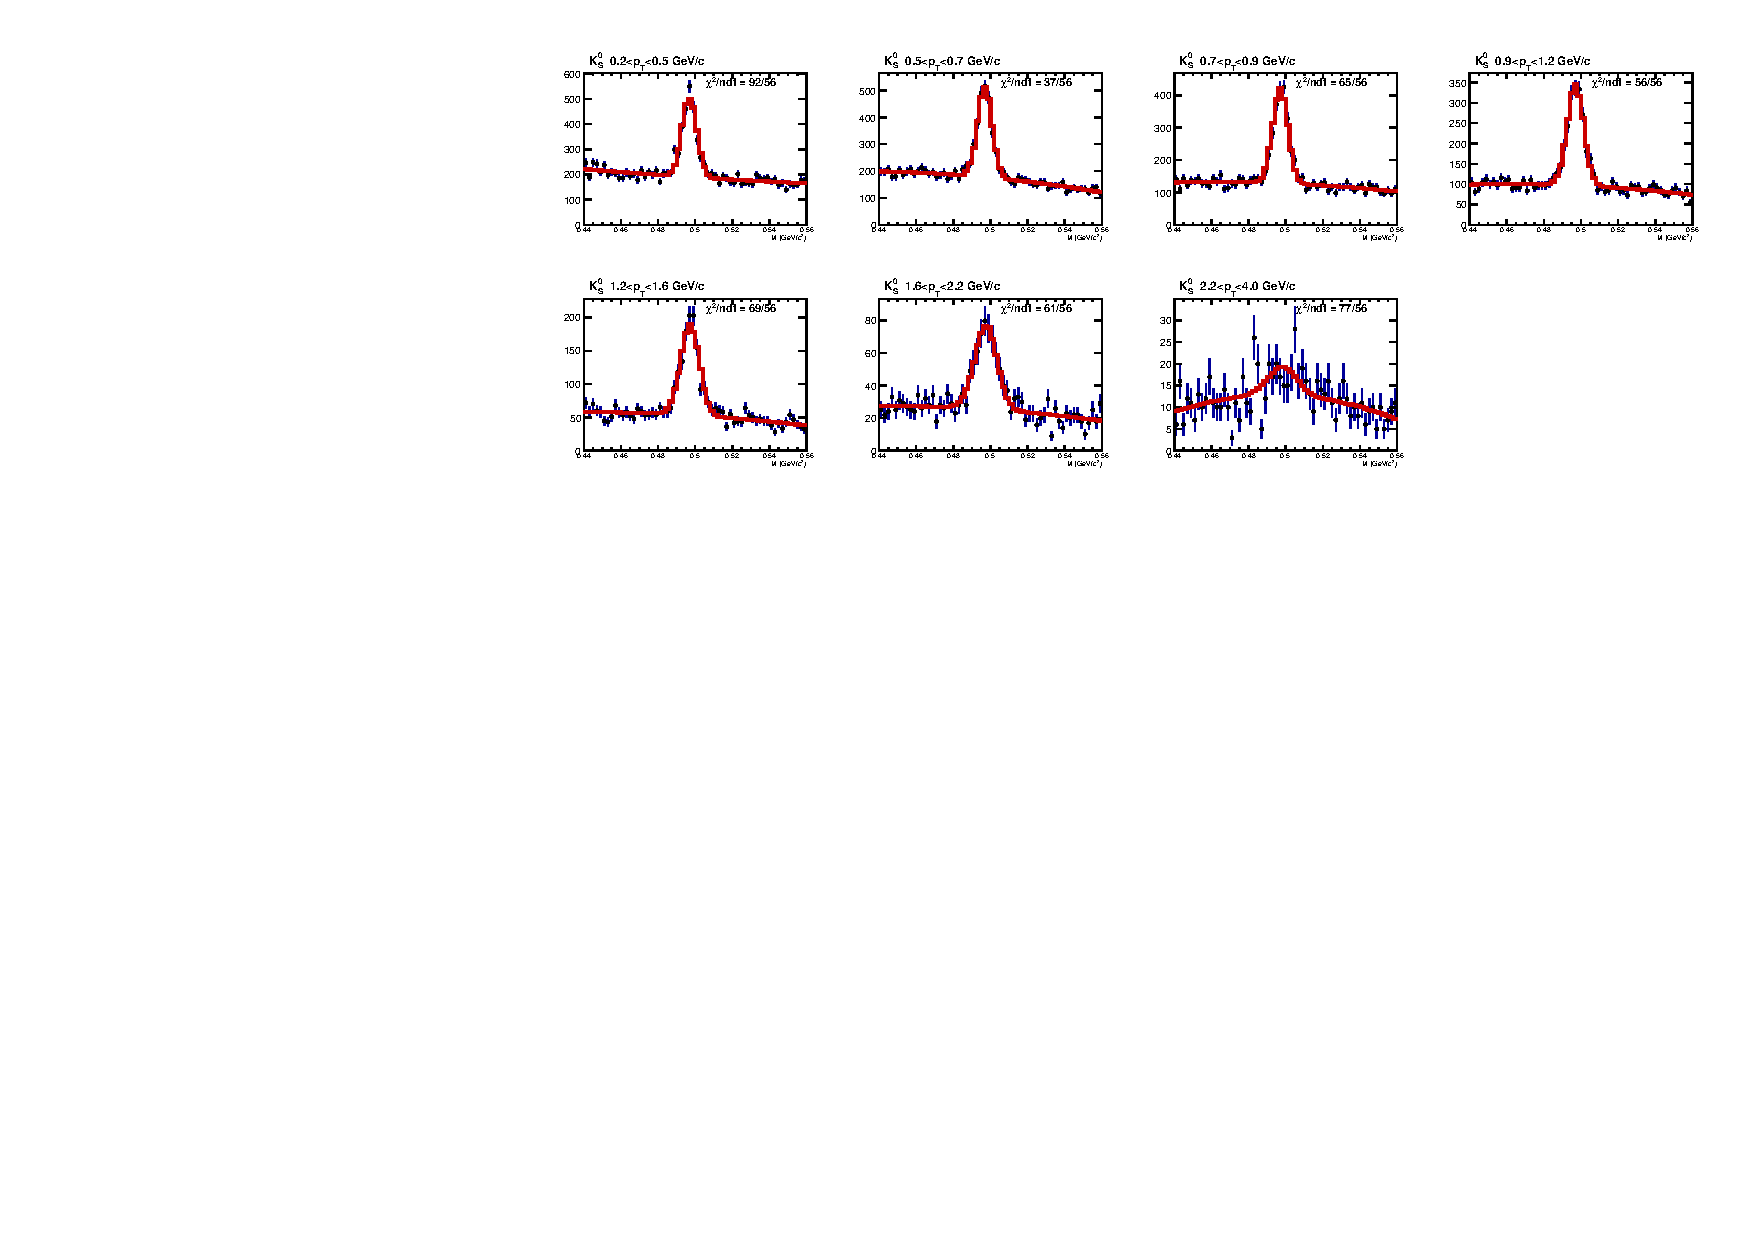
\includegraphics[width=\textwidth]{fig_mass_Ks_B_kappa}
\caption{As Fig.~\ref{fig:massksA}, period B.}
\label{fig:massksB}
\end{figure}

\begin{figure}[H]
\centering
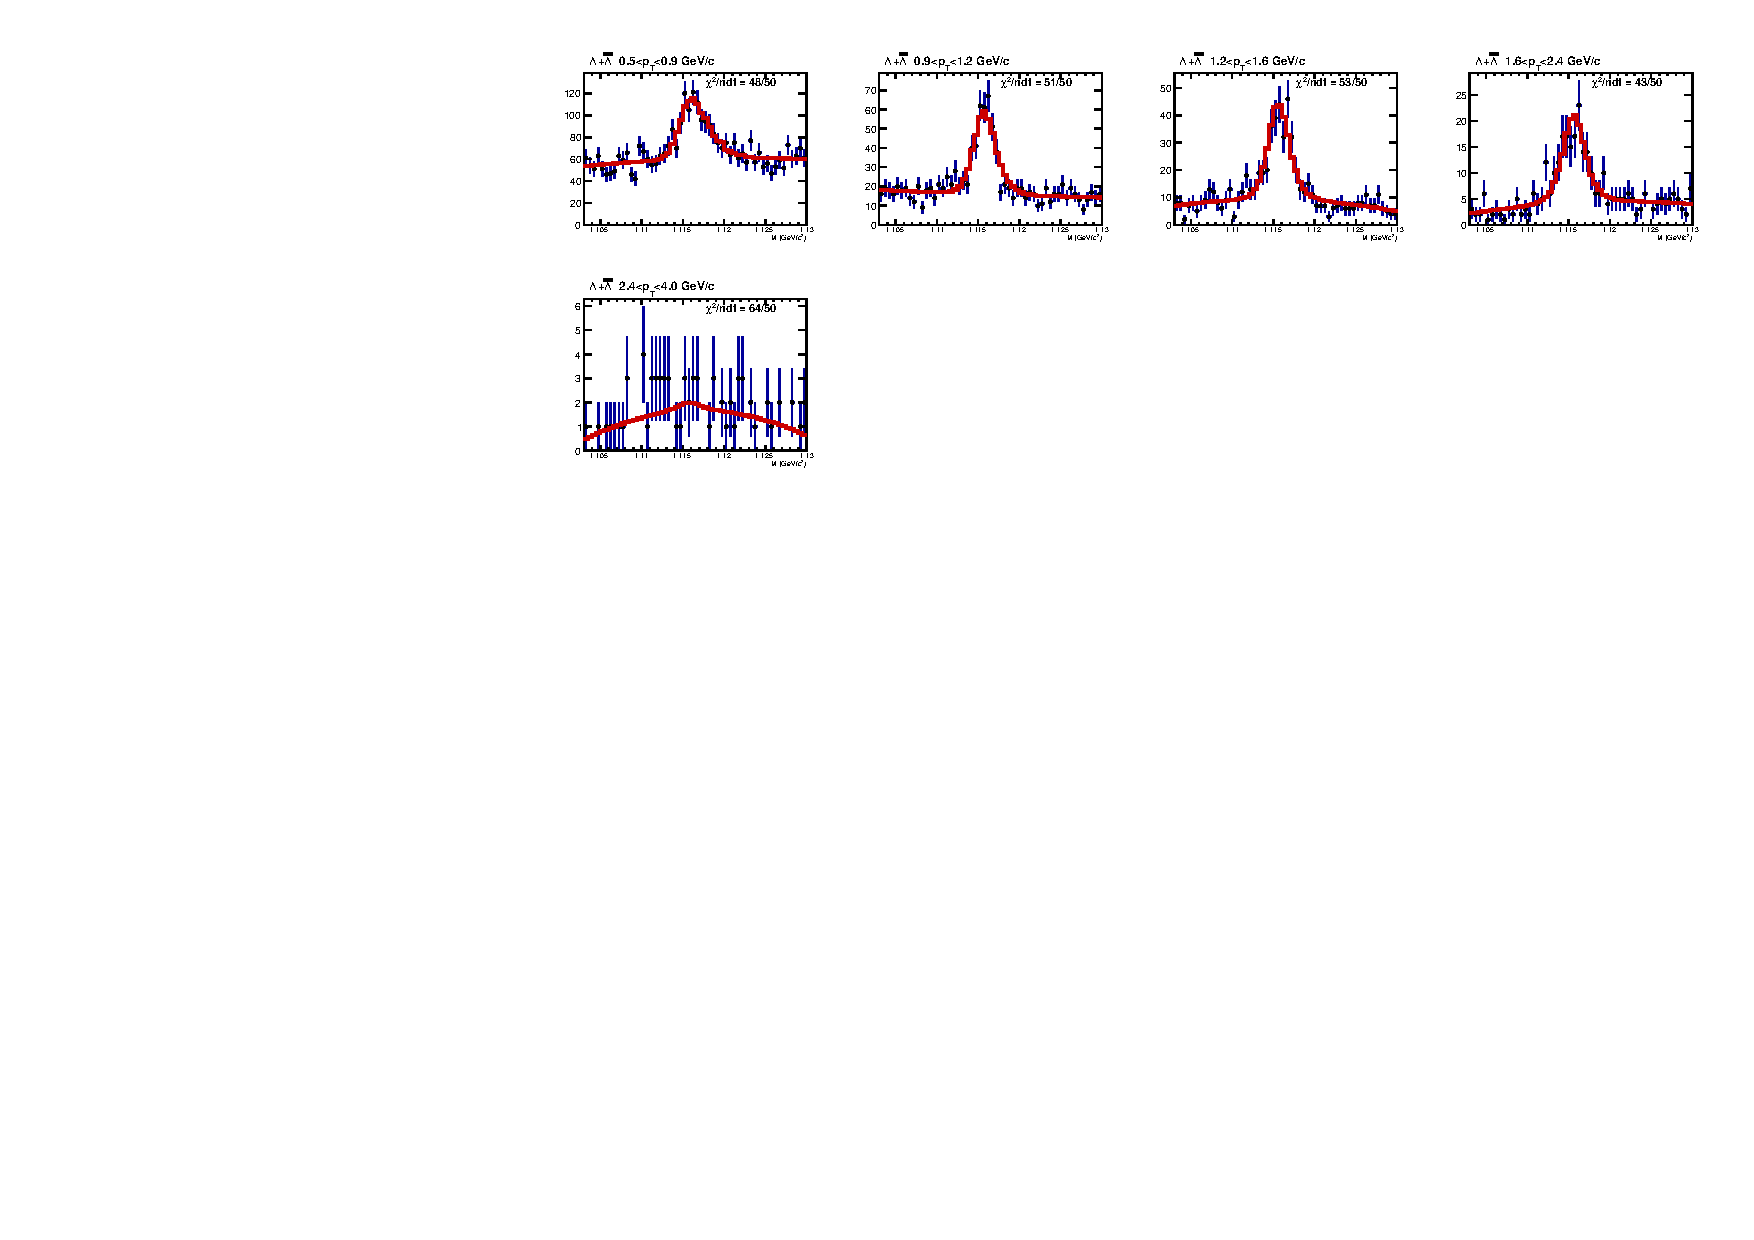
\includegraphics[width=\textwidth]{fig_mass_Lambda_A_kappa}
\caption{\La+$\bar\Lambda$ mass, period A, with $\kappa$; template at the \Ks{} best point (prediction).}
\label{fig:masslaA}
\end{figure}

\begin{figure}[H]
\centering
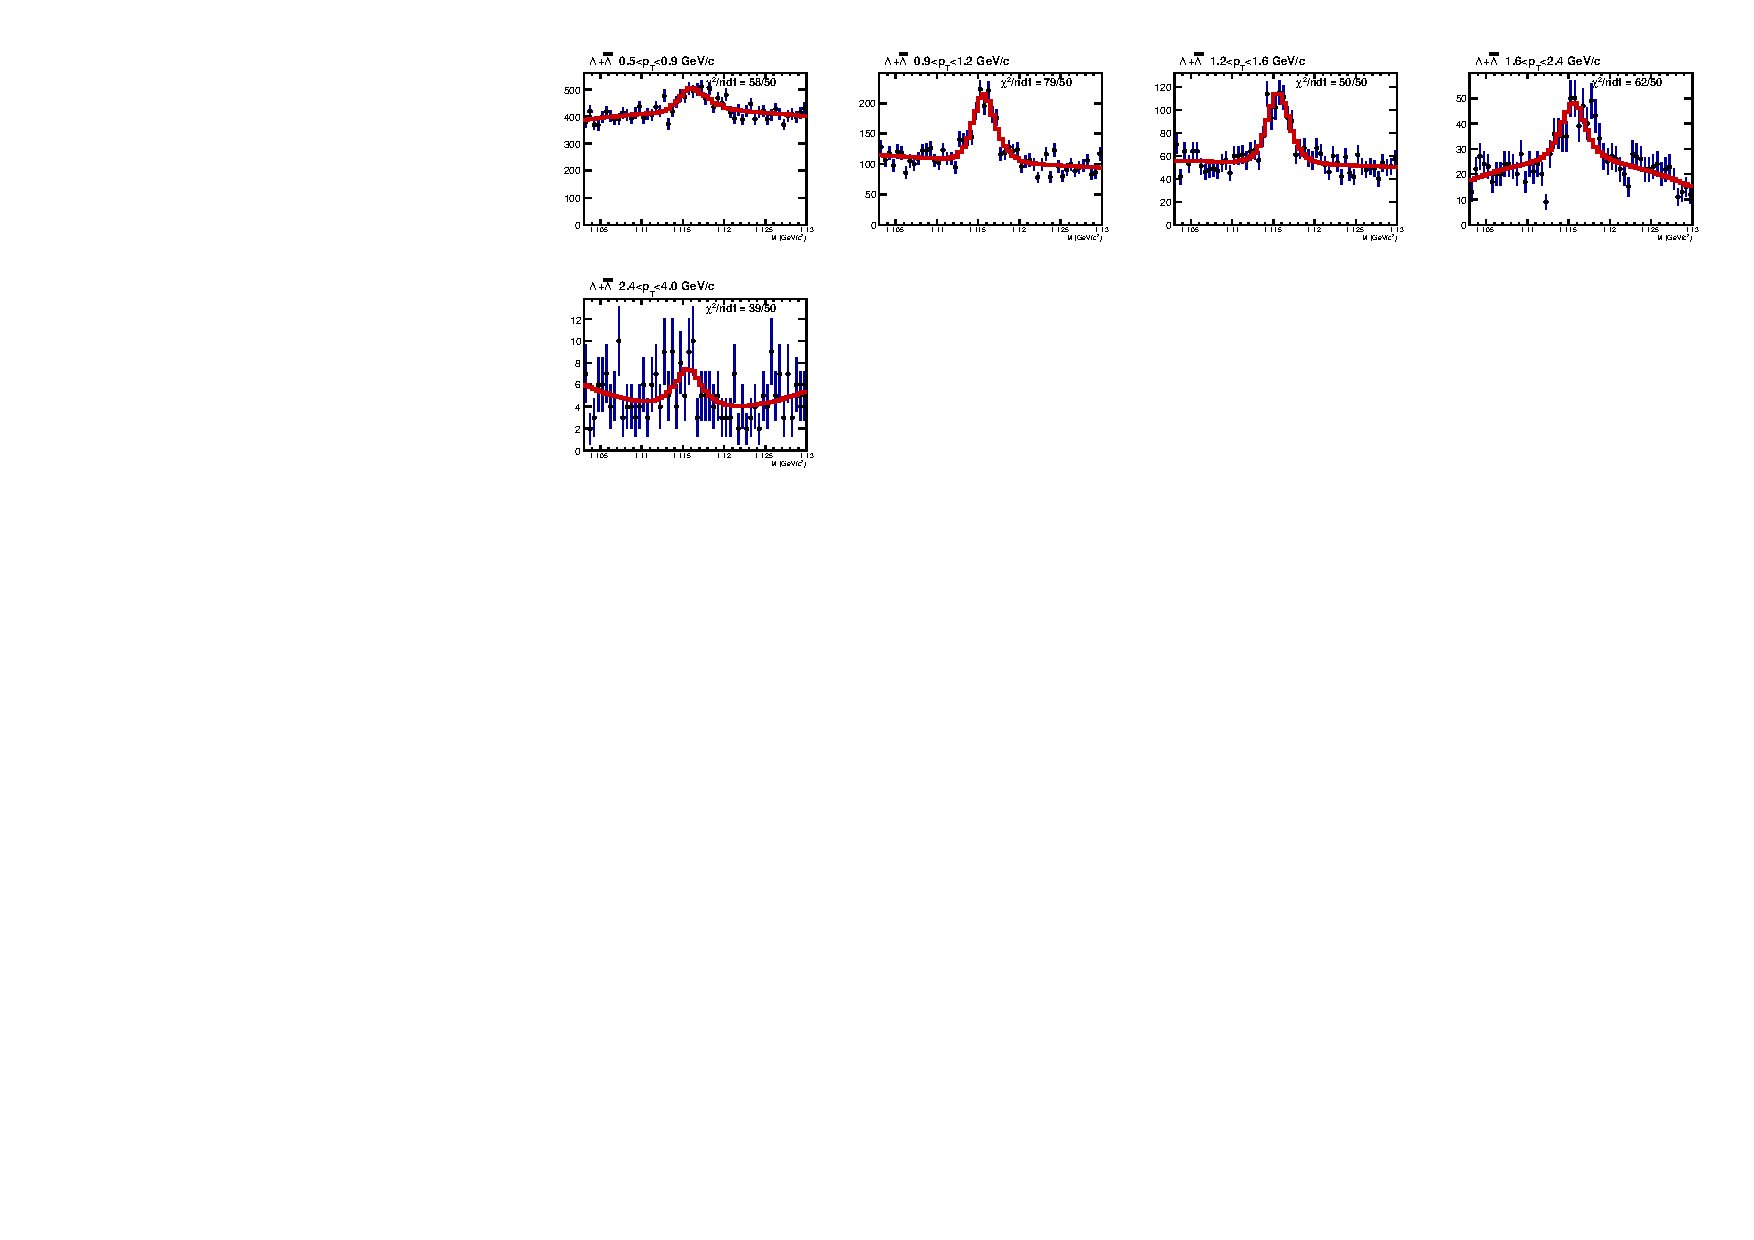
\includegraphics[width=\textwidth]{fig_mass_Lambda_B_kappa}
\caption{As Fig.~\ref{fig:masslaA}, period B.}
\label{fig:masslaB}
\end{figure}

\begin{table}[H]
\centering\small
\caption{Per-bin Baker--Cousins $\chi^2$/ndf of the template fit at the \Ks{} best point of each fit, without and with $\kappa$.}
\label{tab:binchi}
\begin{tabular}{lllcc}
\toprule
period & & V0 \pt{} (GeV/$c$) & no $\kappa$ & with $\kappa$ \\
\midrule
% generated by scripts/make_numbers.py
A & \Ks & 0.2--0.5 & 45.3/56 & 82.2/56 \\
A & \Ks & 0.5--0.7 & 62.4/56 & 64.1/56 \\
A & \Ks & 0.7--0.9 & 59.8/56 & 57.4/56 \\
A & \Ks & 0.9--1.2 & 53.4/56 & 87.3/56 \\
A & \Ks & 1.2--1.6 & 80.6/56 & 59.5/56 \\
A & \Ks & 1.6--2.2 & 79.0/56 & 56.3/56 \\
A & \Ks & 2.2--4.0 & 84.1/56 & 61.6/56 \\
A & \La & 0.5--0.9 & 55.0/50 & 47.9/50 \\
A & \La & 0.9--1.2 & 53.6/50 & 50.7/50 \\
A & \La & 1.2--1.6 & 54.2/50 & 53.0/50 \\
A & \La & 1.6--2.4 & 70.5/50 & 43.4/50 \\
A & \La & 2.4--4.0 & 63.2/50 & 63.7/50 \\
\midrule
B & \Ks & 0.2--0.5 & 75.9/56 & 91.9/56 \\
B & \Ks & 0.5--0.7 & 58.6/56 & 36.8/56 \\
B & \Ks & 0.7--0.9 & 57.0/56 & 65.4/56 \\
B & \Ks & 0.9--1.2 & 66.7/56 & 56.4/56 \\
B & \Ks & 1.2--1.6 & 58.2/56 & 69.1/56 \\
B & \Ks & 1.6--2.2 & 96.4/56 & 61.1/56 \\
B & \Ks & 2.2--4.0 & 60.4/56 & 76.7/56 \\
B & \La & 0.5--0.9 & 52.1/50 & 58.0/50 \\
B & \La & 0.9--1.2 & 80.2/50 & 78.7/50 \\
B & \La & 1.2--1.6 & 60.7/50 & 50.3/50 \\
B & \La & 1.6--2.4 & 67.6/50 & 62.4/50 \\
B & \La & 2.4--4.0 & 57.9/50 & 39.4/50 \\

\bottomrule
\end{tabular}
\end{table}

\section{Tighter \La{} selection}
\label{sec:tight}

The \La{} peak sits on a large combinatorial background (S/B $\approx$ 0.3 within $\pm2\sigma$ with the QA selection), which limits
the precision of its position and makes the \La{} template fits sensitive to the background model. This section tests a tighter
\La{} topological selection, applied identically to data and DDSim templates. \Ks{} is not changed.

\subsection{Choice of the cuts}

\paragraph{Scan.} On run 79509 segments 0--30 (full KFParticle ntuple, KFP mass, $0.5<\pt<4$\gevc;
\fpath{macros/scanLambdaCuts.C}) \ScanNCuts{} combinations of DIRA (0.995--0.9999), $L_{xy}$ (0.5--3~cm), pion and proton
$|{\rm DCA}_{xy}|$ (0.02--0.3 and 0.02--0.1~cm) were evaluated on top of the QA selection. Signal $S$ = counts in
$\pm6$\mevcc{} around the PDG mass minus a linear side-band estimate (1.095--1.104 and 1.128--1.137~GeV/$c^2$), $B$ = that estimate;
figure of merit $S^2/(S+B)$, the effective signal count that sets the error of the peak position. Only cuts that DDSim models are
scanned (no covariance, $\chi^2$ or significance cuts, Sec.~\ref{sec:selection}).
\begin{itemize}
\item QA selection: $S=\ScanBaseS$, $B=\ScanBaseB$, S/B \ScanBaseSB, $S^2/(S+B)=\ScanBaseSeff$.
\item DIRA is the strongest handle: DIRA$>$0.9995 alone gives S/B \ScanDiraSB{} and $S^2/(S+B)=\ScanDiraSeff$ (\ScanDiraKeep\% of
  the signal).
\item A tighter decay length removes signal faster than background: $L_{xy}>2$~cm keeps \ScanLxyKeep\% of the signal
  (S/B \ScanLxySB), because the V0 daughters need silicon hits and therefore decays at small radius.
\item Chosen (\textbf{tight}): QA + DIRA$>$0.9995, $|{\rm DCA}_{xy}(\pi)|>0.10$~cm, $|{\rm DCA}_{xy}(p)|>0.03$~cm: $S=\ScanSelS$
  (\ScanSelKeep\%), $B=\ScanSelB$, S/B \ScanSelSB, $S^2/(S+B)=\ScanSelSeff$ ($\times\ScanGain$). The scan maximum
  (\ScanBestCut, $S^2/(S+B)=\ScanBestSeff$) is within the statistical fluctuation of the scan; the less aggressive DIRA cut was
  preferred (user decision) because the pointing angle is the variable DDSim models least well (Sec.~\ref{sec:open}).
\end{itemize}

\paragraph{Can a tight cut bias the resolution fit?} DDSim applies the selection before the momentum smearing of the fit
(Sec.~\ref{sec:method}). If a tight cut preferentially removed badly measured candidates in data, the data peak would narrow
while the templates would not, and $(a,b)$ would come out too small. Test on the same 31 segments (\fpath{macros/cutBiasTest.C}):
Gaussian width with the QA and the tight selection in data (KFP mass) and in DDSim (templates smeared at the DDSim main point
$a=3.75$\%/(GeV/$c$), $b=1.4$\%, $s=0.991$), for \Ks{} with the same DIRA and pion cuts on both pions and for \La{} with the tight
selection (Table~\ref{tab:tightbias}). The width ratio tight/QA agrees between data and DDSim within the statistics (\Ks{}
\pt-integrated: data $\BiasKsRatD\pm\BiasKsRatDe$, DDSim \BiasKsRatS; \La: $\BiasLaRatD\pm\BiasLaRatDe$ vs \BiasLaRatS). The test
is limited to $\approx$5\% by the 31-segment sample. The DDSim \La{} templates keep \TmplLaTight{} of the candidates
(\TmplLaTightFrac{} of the QA templates).

\begin{table}[H]
\centering\footnotesize
\caption{Cut-bias test on run 79509 segments 0--30: Gaussian width (MeV/$c^2$) with the QA and the tight selection in data
(KFP mass; error of the ratio = quadrature of the two errors, conservative since the tight sample is a subset) and in DDSim at
the main point.}
\label{tab:tightbias}
\begin{tabular}{llcccccc}
\toprule
 & \pt{} (GeV/$c$) & data QA & data tight & data ratio & DDSim QA & DDSim tight & DDSim ratio \\
\midrule
% generated by scripts/make_numbers.py
\Ks & 0.2--0.7 & 4.70$\pm$0.22 & 4.23$\pm$0.15 & 0.899$\pm$0.052 & 4.63 & 4.64 & 1.002 \\
\Ks & 0.7--1.2 & 5.45$\pm$0.32 & 5.47$\pm$0.24 & 1.005$\pm$0.073 & 5.87 & 5.86 & 0.998 \\
\Ks & 1.2--2.2 & 5.95$\pm$0.63 & 6.86$\pm$0.66 & 1.152$\pm$0.165 & 8.39 & 8.23 & 0.981 \\
\Ks & 2.2--4.0 & 7.51$\pm$1.83 & 8.18$\pm$0.27 & 1.090$\pm$0.269 & 13.05 & 12.52 & 0.959 \\
\Ks & 0.2--4.0 & 5.15$\pm$0.17 & 4.94$\pm$0.13 & 0.958$\pm$0.042 & 5.68 & 5.59 & 0.985 \\
\La+$\bar\Lambda$ & 0.5--1.2 & 2.06$\pm$0.30 & 1.90$\pm$0.17 & 0.922$\pm$0.158 & 1.77 & 1.74 & 0.982 \\
\La+$\bar\Lambda$ & 1.2--4.0 & 2.09$\pm$0.53 & 2.21$\pm$0.28 & 1.054$\pm$0.300 & 2.22 & 2.15 & 0.971 \\
\La+$\bar\Lambda$ & 0.5--4.0 & 2.02$\pm$0.27 & 1.99$\pm$0.15 & 0.986$\pm$0.149 & 1.90 & 1.86 & 0.979 \\

\bottomrule
\end{tabular}
\end{table}

\subsection{Production}

The data ntuples of 256 of the 287 segments are not kept (Sec.~\ref{sec:dataset}), so all segments were reprocessed (condor
cluster 481293, \fpath{run3pp/macro/kappa/fill_v0_mass_kappa_v2.C}, \fpath{macro/run_v0mass_kappa_v2.sh}). The v2 fill macro writes,
from the same candidates, all histograms of the first production unchanged, the tight histograms \fcmd{hLa_tight},
\fcmd{hLaBar_tight} in all three mass versions, and a slim candidate tree per segment (pre-selection DIRA$>$0.99,
$L_{xy}>0.2$~cm, $|{\rm DCA}_{xy}|>0.01$~cm; 84~MB for all segments, kept locally in \fpath{data/kappa_v2/v0tree}) so that further
cut variations need no reprocessing. Checks: the v2 macro reproduces the 18 histograms of the first production bin by bin on run
79509 segments 0--30 before submission, and after the production all v1 histograms of all \ReproTwoN{} segments are bin-by-bin
identical to production 480714 (\ChkReproTwo). In \fpath{fitMomRes.C} the option \fcmd{laTight=1} reads the tight data
histograms and applies the same three cuts to the DDSim \La{} templates (\fcmd{rcCosTheta}, \fcmd{rcPiDcaXY}, \fcmd{rcPDcaXY});
the \Ks{} part of the fit is unchanged (identical \Ks{} results: \ChkKsSame).

\subsection{Mass peak}

\begin{figure}[H]
\centering
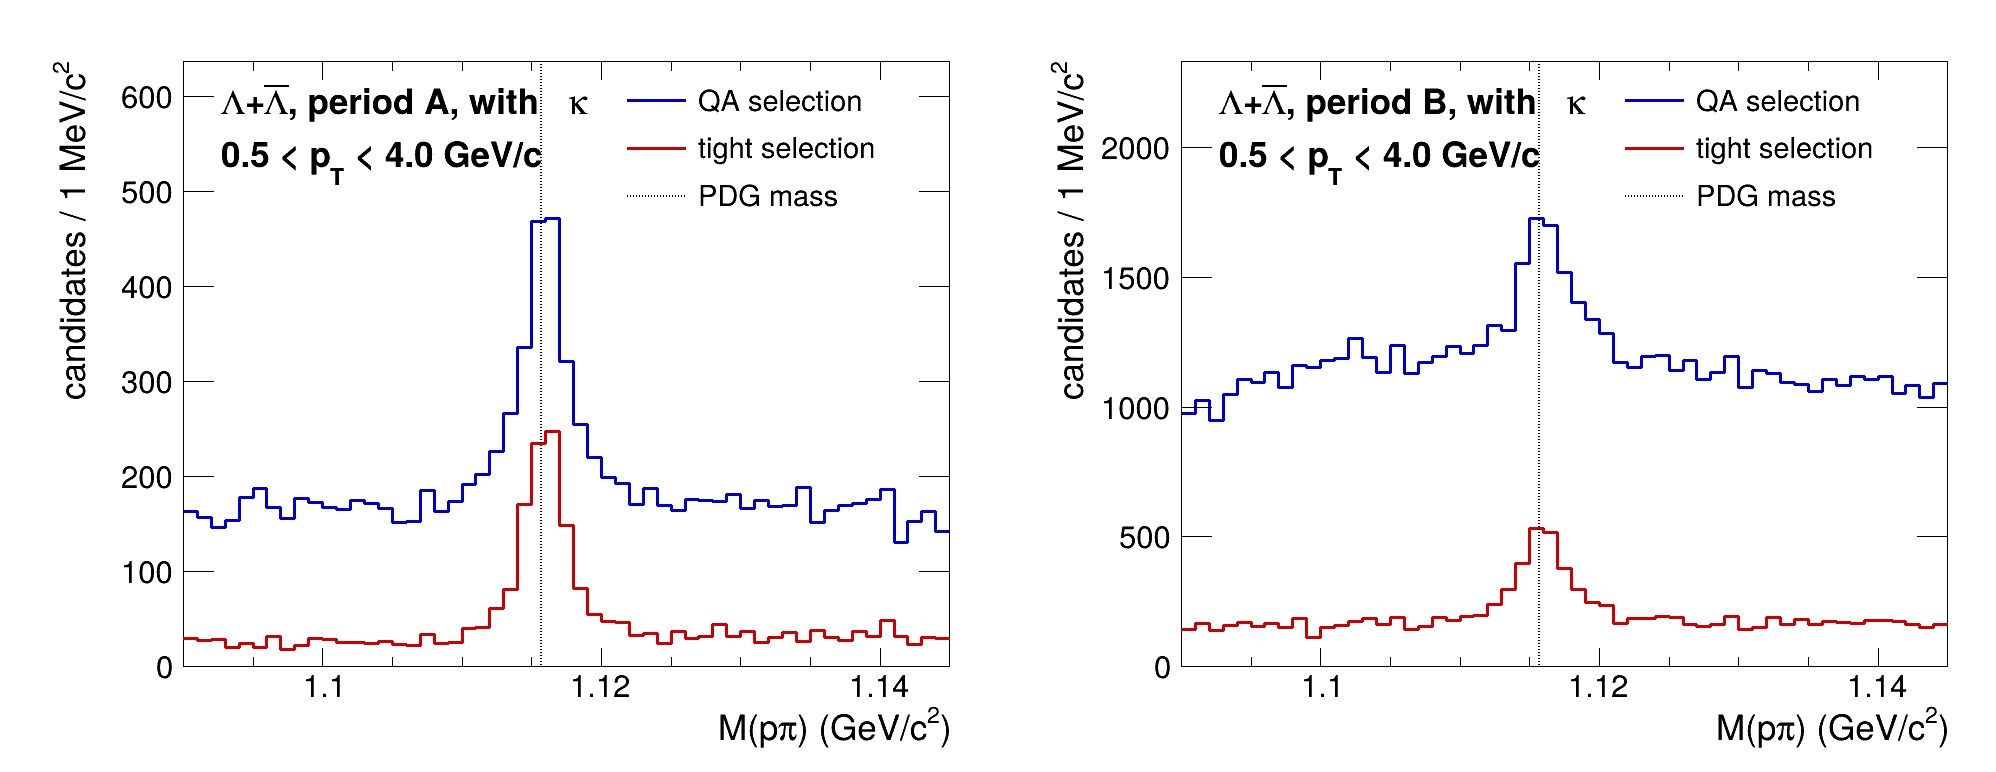
\includegraphics[width=\textwidth]{fig_latight_mass}
\caption{\La+$\bar\Lambda$ mass, recomputed with $\kappa$, $0.5<\pt<4$\gevc, with the QA (blue) and the tight (red) selection;
period A (left) and B (right). Script \fpath{scripts/latight.C}.}
\label{fig:latightmass}
\end{figure}

\begin{table}[H]
\centering\footnotesize
\caption{\La+$\bar\Lambda$ Gaussian peak (gaus + quadratic, 1.103--1.130~GeV/$c^2$, 0.5\mevcc{} bins, likelihood fit),
$0.5<\pt<4$\gevc, QA vs tight selection: mean and width (MeV/$c^2$), S/B within $\pm2\sigma$, and the fraction of the Gaussian
signal kept by the tight cuts. PDG \PdgLa\mevcc. \fpath{macros/laTightPeaks.C}.}
\label{tab:tightpeaks}
\begin{tabular}{llccccccc}
\toprule
 & mass & $M$ QA & $M$ tight & $\sigma$ QA & $\sigma$ tight & S/B QA & S/B tight & kept (\%) \\
\midrule
% generated by scripts/make_numbers.py
A & no $\kappa$ & 1115.55$\pm$0.12 & 1115.65$\pm$0.10 & 2.16 & 2.13 & 0.81 & 3.20 & 71 \\
 & with $\kappa$ & 1115.92$\pm$0.09 & 1115.92$\pm$0.07 & 1.63 & 1.55 & 1.02 & 4.19 & 71 \\
\midrule
B & no $\kappa$ & 1116.24$\pm$0.17 & 1115.93$\pm$0.12 & 2.70 & 2.53 & 0.21 & 0.87 & 57 \\
 & with $\kappa$ & 1116.11$\pm$0.11 & 1115.96$\pm$0.08 & 1.92 & 1.79 & 0.28 & 1.20 & 60 \\
\midrule
all & no $\kappa$ & 1115.99$\pm$0.12 & 1115.81$\pm$0.08 & 2.55 & 2.35 & 0.29 & 1.22 & 61 \\
 & with $\kappa$ & 1116.02$\pm$0.08 & 1115.95$\pm$0.06 & 1.58 & 1.69 & 0.35 & 1.65 & 74 \\

\bottomrule
\end{tabular}
\end{table}

With $\kappa$, the tight selection raises S/B from \PerAllKapLpQaSB{} to \PerAllKapLpTiSB{} (all segments), keeps \PerAllKapLpKeep\%
of the signal (A \PerAKapLpKeep\%, B \PerBKapLpKeep\%) and reduces the error of the peak position from \PerAllKapLpQaMe{} to
\PerAllKapLpTiMe\mevcc{} (A $\PerAKapLpQaMe\to\PerAKapLpTiMe$, B $\PerBKapLpQaMe\to\PerBKapLpTiMe$). The peak stays above the
PDG mass: $\PerAllKapLpTiM\pm\PerAllKapLpTiMe$\mevcc{} (\PerAllKapLpTiAbove\mevcc, $\PerAllKapLpTiPull\sigma$ statistical).

\subsection{Template fits}

\begin{table}[H]
\centering\footnotesize
\caption{\La-only template fit with the QA and the tight \La{} selection, per period and mass version: profile $\Delta\chi^2=1$
intervals, $\chi^2$/ndf, $\Delta\chi^2_\Lambda$ (\La{} $\chi^2$ at the \Ks{} best point minus its minimum), and the joint
\Ks+\La{} best point ($a$ in \%/(GeV/$c$), $b$ in \%, $s$). No best point on the grid edge (\ChkEdgeTight).}
\label{tab:tightfits}
\setlength{\tabcolsep}{3.5pt}
\begin{tabular}{lllccccccc}
\toprule
 & mass & \La{} sel. & $a$ (\%/(GeV/$c$)) & $b$ (\%) & $s$ & $\chi^2$/ndf & $\Delta\chi^2_\Lambda$ & joint $a$, $b$, $s$ \\
\midrule
% generated by scripts/make_numbers.py
A & no $\kappa$ & QA & $4.25^{+0.30}_{-0.18}$ & 1.60 & $0.9910^{+0.0007}_{-0.0009}$ & 293.2/247 & 3.4 & 3.00, 1.60, 0.991 \\
 &  & tight & $4.75^{+0.16}_{-0.18}$ & 1.40 & $0.9930^{+0.0015}_{-0.0012}$ & 244.6/247 & 4.2 & 3.00, 1.60, 0.991 \\
\addlinespace
 & with $\kappa$ & QA & $3.25^{+0.60}_{-0.45}$ & 1.20 & $0.9980^{+0.0022}_{-0.0004}$ & 252.7/247 & 6.1 & 1.50, 1.40, 0.999 \\
 &  & tight & $2.25^{+0.23}_{-0.33}$ & 1.20 & $0.9990^{+0.0014}_{-0.0004}$ & 296.6/247 & 3.4 & 1.50, 1.40, 0.999 \\
\midrule
B & no $\kappa$ & QA & $5.25^{+0.33}_{-0.29}$ & 3.00 & $1.0050^{+0.0009}_{-0.0017}$ & 287.9/247 & 30.5 & 4.00, 1.20, 0.991 \\
 &  & tight & $7.25^{+0.75}_{-0.16}$ & 1.40 & $0.9970^{+0.0021}_{-0.0021}$ & 288.1/247 & 38.3 & 3.75, 1.40, 0.991 \\
\addlinespace
 & with $\kappa$ & QA & $3.50^{+0.16}_{-0.72}$ & 1.40 & $1.0010^{+0.0008}_{-0.0014}$ & 284.0/247 & 4.8 & 2.00, 1.40, 0.998 \\
 &  & tight & $4.25^{+0.52}_{-0.21}$ & 1.20 & $1.0000^{+0.0011}_{-0.0014}$ & 323.9/247 & 11.9 & 2.00, 1.40, 0.998 \\
\midrule
all & no $\kappa$ & QA & $5.25^{+0.52}_{-0.29}$ & 2.00 & $0.9960^{+0.0025}_{-0.0013}$ & 280.5/247 & 25.0 & 3.50, 1.40, 0.991 \\
 &  & tight & $7.75^{+0.14}_{-0.25}$ & 1.00 & $0.9950^{+0.0011}_{-0.0006}$ & 263.5/247 & 45.2 & 3.50, 1.40, 0.991 \\
\addlinespace
 & with $\kappa$ & QA & $2.75^{+0.48}_{-0.63}$ & 1.20 & $1.0000^{+0.0013}_{-0.0011}$ & 255.7/247 & 9.0 & 1.75, 1.40, 0.999 \\
 &  & tight & $4.25^{+0.22}_{-0.31}$ & 1.00 & $0.9990^{+0.0011}_{-0.0003}$ & 309.7/247 & 17.3 & 1.75, 1.40, 0.999 \\

\bottomrule
\end{tabular}
\end{table}

\begin{itemize}
\item \textbf{Scale.} With $\kappa$ and the tight selection the \La-only scale is $s=\PerAKapTiLaS$ (A), \PerBKapTiLaS{} (B)
  and \PerAllKapTiLaS{} (all), consistent with the \Ks{} values (\PerAKapKsS, \PerBKapKsS, \PerAllKapKsS). The half-width of the
  $\Delta\chi^2=1$ interval in $s$ changes from \PerAKapQaLaSW{} to \PerAKapTiLaSW{} (A), \PerBKapQaLaSW{} to \PerBKapTiLaSW{} (B)
  and \PerAllKapQaLaSW{} to \PerAllKapTiLaSW{} (all), in units of $10^{-3}$.
\item \textbf{Resolution, period A.} The tight \La-only curvature term moves towards the \Ks{} value
  ($a=\PerAKapQaLaA\to\PerAKapTiLaA$ vs \Ks{} \PerAKapKsA\%/(GeV/$c$)); $\Delta\chi^2_\Lambda=\PerAKapQaDchi\to\PerAKapTiDchi$.
\item \textbf{Resolution, period B.} The tight \La-only $a$ rises ($\PerBKapQaLaA\to\PerBKapTiLaA$) and the \La/\Ks{} tension grows
  ($\Delta\chi^2_\Lambda=\PerBKapQaDchi\to\PerBKapTiDchi$; all segments $\PerAllKapQaDchi\to\PerAllKapTiDchi$); the \La{} $\chi^2$
  worsens (\PerBKapQaLaChi{} $\to$ \PerBKapTiLaChi/247). Table~\ref{tab:tightwidths}: at 1.2--1.6 and 1.6--2.4\gevc{} the tight data peaks are wider than the tight
  templates at the \Ks{} best point by \WidTiOne{} and \WidTiTwo{} standard deviations of the data width (QA selection:
  \WidQaOne{} and \WidQaTwo).
\item With $\kappa$ the joint \Ks+\La{} best points are unchanged by the tighter \La{} selection (\Ks{} dominates); without
  $\kappa$ the period-B joint point moves by one grid step in $a$ and $b$.
\end{itemize}

\begin{table}[H]
\centering\footnotesize
\caption{\La{} Gaussian width in data / in the template at the \Ks{} best point (MeV/$c^2$), per V0-\pt{} bin, with $\kappa$,
QA vs tight selection (from the template-fit display fits, \fcmd{BIN} rows of the fit logs; ``--'' = data fit unconstrained or at its 0.3\mevcc{} lower limit).}
\label{tab:tightwidths}
\begin{tabular}{llccccc}
\toprule
 & sel. & 0.5--0.9 & 0.9--1.2 & 1.2--1.6 & 1.6--2.4 & 2.4--4.0 \\
\midrule
% generated by scripts/make_numbers.py
A & QA & 2.01$\pm$0.24 / 1.70 & 1.04$\pm$0.10 / 1.48 & 1.73$\pm$0.17 / 1.45 & 1.98$\pm$0.24 / 1.57 & -- / 1.91 \\
 & tight & 1.63$\pm$0.14 / 1.68 & 1.10$\pm$0.07 / 1.44 & 1.47$\pm$0.14 / 1.43 & 1.41$\pm$0.19 / 1.52 & -- / 1.84 \\
\midrule
B & QA & 2.24$\pm$0.32 / 1.74 & 1.39$\pm$0.13 / 1.53 & 1.49$\pm$0.17 / 1.56 & 1.94$\pm$0.19 / 1.77 & 2.08$\pm$0.85 / 2.29 \\
 & tight & -- / 1.70 & 1.32$\pm$0.10 / 1.50 & 1.73$\pm$0.15 / 1.53 & 2.11$\pm$0.20 / 1.72 & -- / 2.19 \\

\bottomrule
\end{tabular}
\end{table}

\begin{figure}[H]
\centering
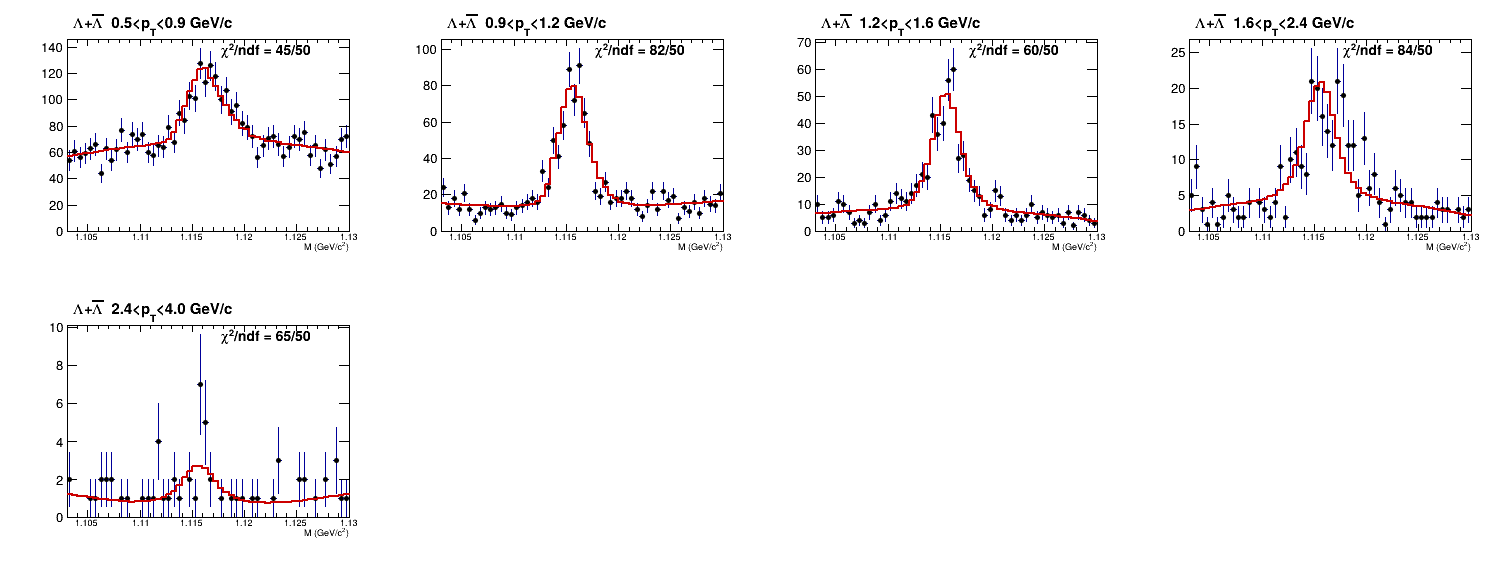
\includegraphics[width=\textwidth]{fig_mass_Lambda_B_tight}
\caption{\La+$\bar\Lambda$ mass, period B, with $\kappa$ and the tight selection; template at the \Ks{} best point (prediction).
Compare Fig.~\ref{fig:masslaB} (QA selection).}
\label{fig:masslaBtight}
\end{figure}

\choice{\textbf{Use of the tight selection} (adopted): the tight \La{} selection is used for the \La{} peak position and the
\La{} momentum scale ($s_\Lambda$ with $\kappa$: \PerAKapTiLaS, \PerBKapTiLaS, \PerAllKapTiLaS{} for A, B, all). The resolution
$(a,b)$ stays determined by \Ks{} (Table~\ref{tab:summary}); the \La{} resolution with the tight selection is not used until the
period-B width mismatch is understood (Sec.~\ref{sec:open}).}

\caveat{Why the tight templates under-predict the period-B width above 1.2\gevc{} is not established. Candidates: the pointing
angle is too good in DDSim (true PV, unsmeared directions; in the full-simulation closure study 5\% of the true \Ks{} have DIRA$<$0.995 against 0.1\% in DDSim), so a
DIRA$>$0.9995 cut selects different decay topologies in data and DDSim; higher pile-up in period B; statistics (the 2.4--4\gevc{}
bin has $\approx$10 tight signal candidates in B). The 31-segment bias test (period A only) shows no effect at the 5\% level.}

\section{Run dependence}
\label{sec:rundep}

The period split was motivated by the observation that the fitted curvature term differs between subsets of the sample. Fits with
the KFP mass (no $\kappa$) on run groups (Table~\ref{tab:groups}) and per-run counts (Table~\ref{tab:runs}) show:
\begin{itemize}
\item $a$ grows with the run period: \GrpThirtyOne\%/(GeV/$c$) on run 79509 segments 0--30, \PerAKfpKsA{} on period A,
  \GrpNine{} on runs 80904--80915 and \GrpEightOne{} on runs 81556--81609;
\item the number of \Ks{} QA candidates per event (signal plus combinatorial background) grows in the same order:
  \PerAKsEvMin--\PerAKsEvMax{} per run in period A and \PerBKsEvMin--\PerBKsEvMax{} in period B. This points to higher
  luminosity or pile-up in the later runs; the luminosity itself is not checked here.
\end{itemize}
A luminosity-dependent effect such as TPC space-charge distortions would produce this pattern, but this note does not test the
hypothesis. The $\kappa$ table, derived in period A, removes the same fraction of $a$ in both periods (Sec.~\ref{sec:results}).

\begin{table}[H]
\centering\small
\caption{\Ks{} fit with the KFP mass on run groups (same method; $s$ grid 0.975--1.015). Statistical intervals only. Logs
\fpath{logs/fitMomRes_{kfp31,g7951x,g809xx,g81xxx,k287_*_kfp}.txt}.}
\label{tab:groups}
\begin{tabular}{lcccc}
\toprule
runs & $a$ (\%/(GeV/$c$)) & $b$ (\%) & $s$ & $\chi^2$/ndf \\
\midrule
% generated by scripts/make_numbers.py
79509 seg.\ 0--30 & $2.00^{+0.76}_{-0.26}$ & $1.80^{+0.07}_{-0.24}$ & 0.990 & 427.2/389 \\
79509--79516 (A) & $3.00^{+0.06}_{-0.27}$ & $1.60^{+0.03}_{-0.05}$ & 0.991 & 470.4/389 \\
79510--79516 & $3.00^{+0.13}_{-0.15}$ & $1.60^{+0.02}_{-0.16}$ & 0.991 & 510.2/389 \\
80904--80915 & $3.75^{+0.18}_{-0.34}$ & $1.20^{+0.10}_{-0.10}$ & 0.991 & 395.6/389 \\
81556--81609 & $4.25^{+0.79}_{-0.31}$ & $1.40^{+0.10}_{-0.48}$ & 0.990 & 427.4/389 \\
B (all non-A) & $4.00^{+0.29}_{-0.18}$ & $1.20^{+0.15}_{-0.05}$ & 0.991 & 400.5/389 \\
all & $3.75^{+0.07}_{-0.27}$ & $1.40^{+0.05}_{-0.05}$ & 0.991 & 421.5/389 \\

\bottomrule
\end{tabular}
\end{table}

\begin{table}[H]
\centering\scriptsize
\caption{Per run: period, segments, processed events, \Ks{} QA candidates (all masses in 0.40--0.60~GeV/$c^2$, signal + background)
and per event, \La+$\bar\Lambda$ QA candidates, and mean $\kappa$ of the QA candidates (\Ks{} $\pi^-$, $\pi^+$; \La{} pion,
proton). From the condor job logs (\fpath{logs/joblines.txt}).}
\label{tab:runs}
\setlength{\tabcolsep}{3.5pt}
\begin{tabular}{rcrrrcrcccc}
\toprule
run & per. & seg. & events & \Ks{} cand. & \Ks/ev & \La{} cand. & $\kappa_{\pi^-}$ & $\kappa_{\pi^+}$ & $\kappa_{\pi}^{\Lambda}$ & $\kappa_{p}^{\Lambda}$ \\
\midrule
% generated by scripts/make_numbers.py
79509 & A & 39 & 38{,}656 & 8{,}939 & 0.231 & 17{,}656 & 0.9980 & 1.0164 & 1.0078 & 1.0067 \\
79510 & A & 8 & 7{,}931 & 1{,}599 & 0.202 & 3{,}306 & 0.9978 & 1.0160 & 1.0077 & 1.0067 \\
79511 & A & 8 & 7{,}934 & 1{,}717 & 0.216 & 3{,}324 & 0.9980 & 1.0160 & 1.0076 & 1.0063 \\
79512 & A & 8 & 7{,}932 & 1{,}663 & 0.210 & 3{,}087 & 0.9969 & 1.0167 & 1.0076 & 1.0063 \\
79513 & A & 8 & 7{,}931 & 1{,}619 & 0.204 & 2{,}942 & 0.9975 & 1.0164 & 1.0079 & 1.0063 \\
79514 & A & 8 & 7{,}931 & 1{,}493 & 0.188 & 2{,}783 & 0.9977 & 1.0161 & 1.0076 & 1.0063 \\
79515 & A & 8 & 7{,}930 & 1{,}473 & 0.186 & 2{,}623 & 0.9974 & 1.0160 & 1.0079 & 1.0052 \\
79516 & A & 8 & 7{,}928 & 1{,}338 & 0.169 & 2{,}379 & 0.9987 & 1.0162 & 1.0076 & 1.0072 \\
80904 & B & 8 & 7{,}936 & 3{,}778 & 0.476 & 8{,}545 & 0.9971 & 1.0160 & 1.0076 & 1.0063 \\
80905 & B & 8 & 7{,}938 & 3{,}572 & 0.450 & 8{,}029 & 0.9974 & 1.0162 & 1.0078 & 1.0064 \\
80906 & B & 8 & 7{,}938 & 3{,}601 & 0.454 & 7{,}882 & 0.9974 & 1.0160 & 1.0077 & 1.0066 \\
80908 & B & 8 & 7{,}939 & 3{,}036 & 0.382 & 6{,}692 & 0.9983 & 1.0158 & 1.0075 & 1.0066 \\
80909 & B & 8 & 7{,}936 & 2{,}666 & 0.336 & 6{,}117 & 0.9968 & 1.0162 & 1.0077 & 1.0058 \\
80913 & B & 8 & 7{,}930 & 2{,}166 & 0.273 & 4{,}397 & 0.9971 & 1.0162 & 1.0077 & 1.0060 \\
80915 & B & 8 & 7{,}933 & 1{,}994 & 0.251 & 3{,}796 & 0.9972 & 1.0161 & 1.0073 & 1.0064 \\
81556 & B & 8 & 7{,}936 & 7{,}515 & 0.947 & 17{,}241 & 0.9978 & 1.0163 & 1.0076 & 1.0068 \\
81558 & B & 8 & 7{,}937 & 7{,}086 & 0.893 & 16{,}020 & 0.9981 & 1.0163 & 1.0077 & 1.0070 \\
81560 & B & 8 & 7{,}941 & 4{,}724 & 0.595 & 10{,}797 & 0.9980 & 1.0157 & 1.0077 & 1.0068 \\
81562 & B & 8 & 7{,}939 & 4{,}152 & 0.523 & 9{,}505 & 0.9980 & 1.0162 & 1.0077 & 1.0067 \\
81566 & B & 8 & 7{,}933 & 3{,}116 & 0.393 & 6{,}854 & 0.9975 & 1.0159 & 1.0078 & 1.0062 \\
81575 & B & 8 & 7{,}938 & 6{,}779 & 0.854 & 16{,}118 & 0.9978 & 1.0165 & 1.0079 & 1.0069 \\
81576 & B & 8 & 7{,}936 & 6{,}319 & 0.796 & 14{,}385 & 0.9977 & 1.0162 & 1.0077 & 1.0068 \\
81577 & B & 8 & 7{,}937 & 6{,}031 & 0.760 & 13{,}923 & 0.9979 & 1.0165 & 1.0077 & 1.0069 \\
81580 & B & 8 & 7{,}940 & 4{,}564 & 0.575 & 10{,}359 & 0.9978 & 1.0156 & 1.0076 & 1.0066 \\
81581 & B & 8 & 7{,}940 & 4{,}384 & 0.552 & 9{,}782 & 0.9979 & 1.0165 & 1.0077 & 1.0069 \\
81583 & B & 8 & 7{,}937 & 3{,}930 & 0.495 & 8{,}828 & 0.9977 & 1.0165 & 1.0079 & 1.0064 \\
81584 & B & 8 & 7{,}939 & 3{,}446 & 0.434 & 7{,}746 & 0.9978 & 1.0160 & 1.0078 & 1.0061 \\
81585 & B & 8 & 7{,}933 & 3{,}335 & 0.420 & 7{,}403 & 0.9983 & 1.0159 & 1.0078 & 1.0067 \\
81586 & B & 8 & 7{,}931 & 3{,}403 & 0.429 & 7{,}605 & 0.9981 & 1.0159 & 1.0079 & 1.0065 \\
81600 & B & 8 & 7{,}935 & 7{,}773 & 0.980 & 18{,}212 & 0.9974 & 1.0163 & 1.0078 & 1.0066 \\
81601 & B & 8 & 7{,}937 & 6{,}193 & 0.780 & 14{,}406 & 0.9977 & 1.0161 & 1.0076 & 1.0067 \\
81609 & B & 8 & 7{,}936 & 3{,}855 & 0.486 & 8{,}527 & 0.9972 & 1.0160 & 1.0078 & 1.0064 \\

\bottomrule
\end{tabular}
\end{table}

\section{Audit}
\label{sec:audit}

\paragraph{Checks that passed (script-computed, \fpath{scripts/make_numbers.py}).}
\begin{itemize}
\item Jobs: \JobsOk/\JobsN{} condor jobs printed ``OK'' with three non-empty outputs (\fpath{logs/joblines.txt}): \ChkJobs.
\item Reproducibility: in all \ReproN{} segments the KFP-mass histograms of this production (\fcmd{hKs_qa}, \fcmd{hKs_loose},
  \La+$\bar\Lambda$ QA) are bin-by-bin identical to the earlier covariance-free production 480608 (\ReproSame/\ReproN;
  \fpath{run3pp/output/v0mass_kappa_validate/cmpKfpRepro.C}): \ChkRepro.
\item Fill macro: the cluster macro \fpath{fill_v0_mass_kappa.C}, run on the stored run 79509 segment 0--30 ntuples, gives
  bin-by-bin the same \ChkFillN{} histograms (3 versions $\times$ 6) as the independent local implementation
  \fpath{macros/fillV0MassCorr.C} (\fpath{macros/cmpKappaFill.C}): \ChkFill.
\item $\kappa$ table complete (\TabRows{} = \TabNq$\times$\TabNpt$\times$\TabNeta$\times$\TabNphi{} nodes, none missing):
  \ChkTable; interpolation at table nodes returns the node value ($q=\pm1$, $\pt=1$\gevc, $\eta=\varphi=0$): \ChkInterp.
\item Tight-\La{} production 481293: all v1 histograms of the \ReproTwoN{} segments bin-by-bin identical to 480714: \ChkReproTwo;
  \Ks{} fit results identical with and without the tight \La{} option: \ChkKsSame; no tight-fit best point on the grid edge:
  \ChkEdgeTight.
\item No \Ks{} or joint best point on the grid boundary in the fits of Table~\ref{tab:fits}: \ChkEdge.
\end{itemize}

\paragraph{Not verified (assumptions).}
\begin{itemize}
\item That the KFParticle secondary-vertex-constrained daughter momenta are the kinematics the $\kappa$ table was trained on.
\item That the table holds outside runs 79509--79516 (period B); the improvement there is the only evidence.
\item The effect of keeping the uncorrected DIRA, $L_{xy}$ and DCA values in the selection (the correction changes the V0
  direction slightly).
\item Double counting of the proton scale: the templates contain the full-simulation proton bias $\delta_p$, and $\kappa$ corrects
  the measured proton momentum as well.
\item The DCA$_{12}$ cut of the templates (0.2~cm unconstrained) vs the effective data cut (Sec.~\ref{sec:selection}).
\item That all V0 daughters are silicon-matched (seen in the earlier run3pp topology study through the crossing requirement; not
  rechecked on this production, which keeps only histograms).
\item Background shape: quadratic in every bin; no variation in this note (the DDSim calibration found the \La{} result
  sensitive to it).
\end{itemize}

\section{Open issues}
\label{sec:open}

\begin{enumerate}
\item {[decision]} Adoption of the correction in DDSim. If the $\kappa$-corrected response is the target, DDSim needs
  per-period $(a,b,s)$ (Table~\ref{tab:summary}, ``with $\kappa$'') and the analyses must apply $\kappa$ to their data tracks;
  the current DDSim defaults ($a=3.75$\%/(GeV/$c$), $b=1.40$\%, $s=0.991$) describe uncorrected data averaged over all runs.
\item Period B keeps a larger curvature term after the correction (\PerBKapKsA{} vs \PerAKapKsA\%/(GeV/$c$)). A table derived on
  period-B runs, or a per-run fit, would show whether the remainder is a run-dependent distortion that $\kappa$ does not describe.
\item KFP mass vs recomputed mass: in period B the \Ks{} $\chi^2$ is \PerBKfpKsChi{} with the KFP mass and \PerBRawKsChi{} with the
  recomputed mass (best points $(a,b,s)$ = (\PerBKfpKsA\%/(GeV/$c$), \PerBKfpKsB\%, \PerBKfpKsS) and
  (\PerBRawKsA, \PerBRawKsB, \PerBRawKsS)); in period A the two are similar (\PerAKfpKsChi{} vs \PerARawKsChi). The cause
  (vertex-fit treatment, background shape of the recomputed spectrum) is not understood.
\item Residual \Ks{} peak offset with $\kappa$: \PerAKapKsBelow{} (A) and \PerBKapKsBelow\mevcc{} (B) below PDG; fitted
  $s=\PerAKapKsS$ and \PerBKapKsS.
\item Proton scale: check whether $\delta_p$ in the templates should be removed when $\kappa$ is applied (\La-only $s$ with
  $\kappa$: \PerAKapLaS{} and \PerBKapLaS).
\item Tight \La{} selection in period B: the tight data peaks above 1.2\gevc{} are wider than the tight templates
  ($\Delta\chi^2_\Lambda$ \PerBKapQaDchi{} $\to$ \PerBKapTiDchi). Next step (local, slim trees): refill with DIRA alone and with the DCA
  cuts alone to locate the cause, and compare the DIRA distribution of side-band-subtracted \La{} in data and DDSim.
\item \La{} peak position with $\kappa$ and tight selection \PerAllKapLpTiAbove\mevcc{} above PDG
  ($\PerAllKapLpTiPull\sigma$ statistical) while \Ks{} is \PerAKapKsBelow{} (A) and \PerBKapKsBelow\mevcc{} (B) below: the proton scale (item~5) is the first
  suspect.
\item Background-model and window variations, as in the DDSim main calibration, have not been redone with the corrected masses.
\item Regenerate the templates with the current DDSim defaults (DCA$_{12}<0.5$~cm, seeding factor) and refit.
\end{enumerate}

\decision{Which response should DDSim use? Options: (a) keep the uncorrected all-run defaults; (b) adopt the $\kappa$-corrected
response per period (requires the analyses to correct their data with $\kappa$); (c) wait for a $\kappa$ table covering period B.}

\section{Glossary}
\label{sec:glossary}

\begin{description}\itemsep0pt
\item[$\kappa$] per-track multiplier of the transverse momentum from the look-up table, $\pt^{\rm corr}=\kappa\pt$.
\item[$a$, $b$, $s$] curvature term, multiple-scattering term and global scale of the momentum response, Eq.~\ref{eq:model}.
\item[period A / B] runs 79509--79516 (range of the table) / all other runs of the sample.
\item[KFP / no $\kappa$ / with $\kappa$] the three mass versions: KFParticle fitted mass; recomputed from the stored daughter
  momenta; recomputed after the correction.
\item[DDSim] data-driven fast simulation of two-body V0 decays (DataDrivenSim project).
\item[DIRA] cosine of the angle between the V0 momentum and the PV-to-SV flight direction.
\item[DCA$_{12}$, DCA$_{xy}$] distance of closest approach between the daughters; transverse DCA of a daughter to the PV.
\item[$L_{xy}$] transverse decay length (PV to SV).
\item[QA cuts] offline V0 selection of Table~\ref{tab:sel}.
\item[tight \La{} selection] QA + DIRA$>$0.9995, $|{\rm DCA}_{xy}(\pi)|>0.10$, $|{\rm DCA}_{xy}(p)|>0.03$~cm (Sec.~\ref{sec:tight}).
\item[Baker--Cousins $\chi^2$] $2\sum_i[\mu_i-d_i+d_i\ln(d_i/\mu_i)]$, the Poisson likelihood-ratio goodness of fit.
\item[segment] one DST file of a run, about 990 events.
\end{description}

\appendix
\section{Template fits without the correction}
\label{app:raw}

\begin{figure}[H]
\centering
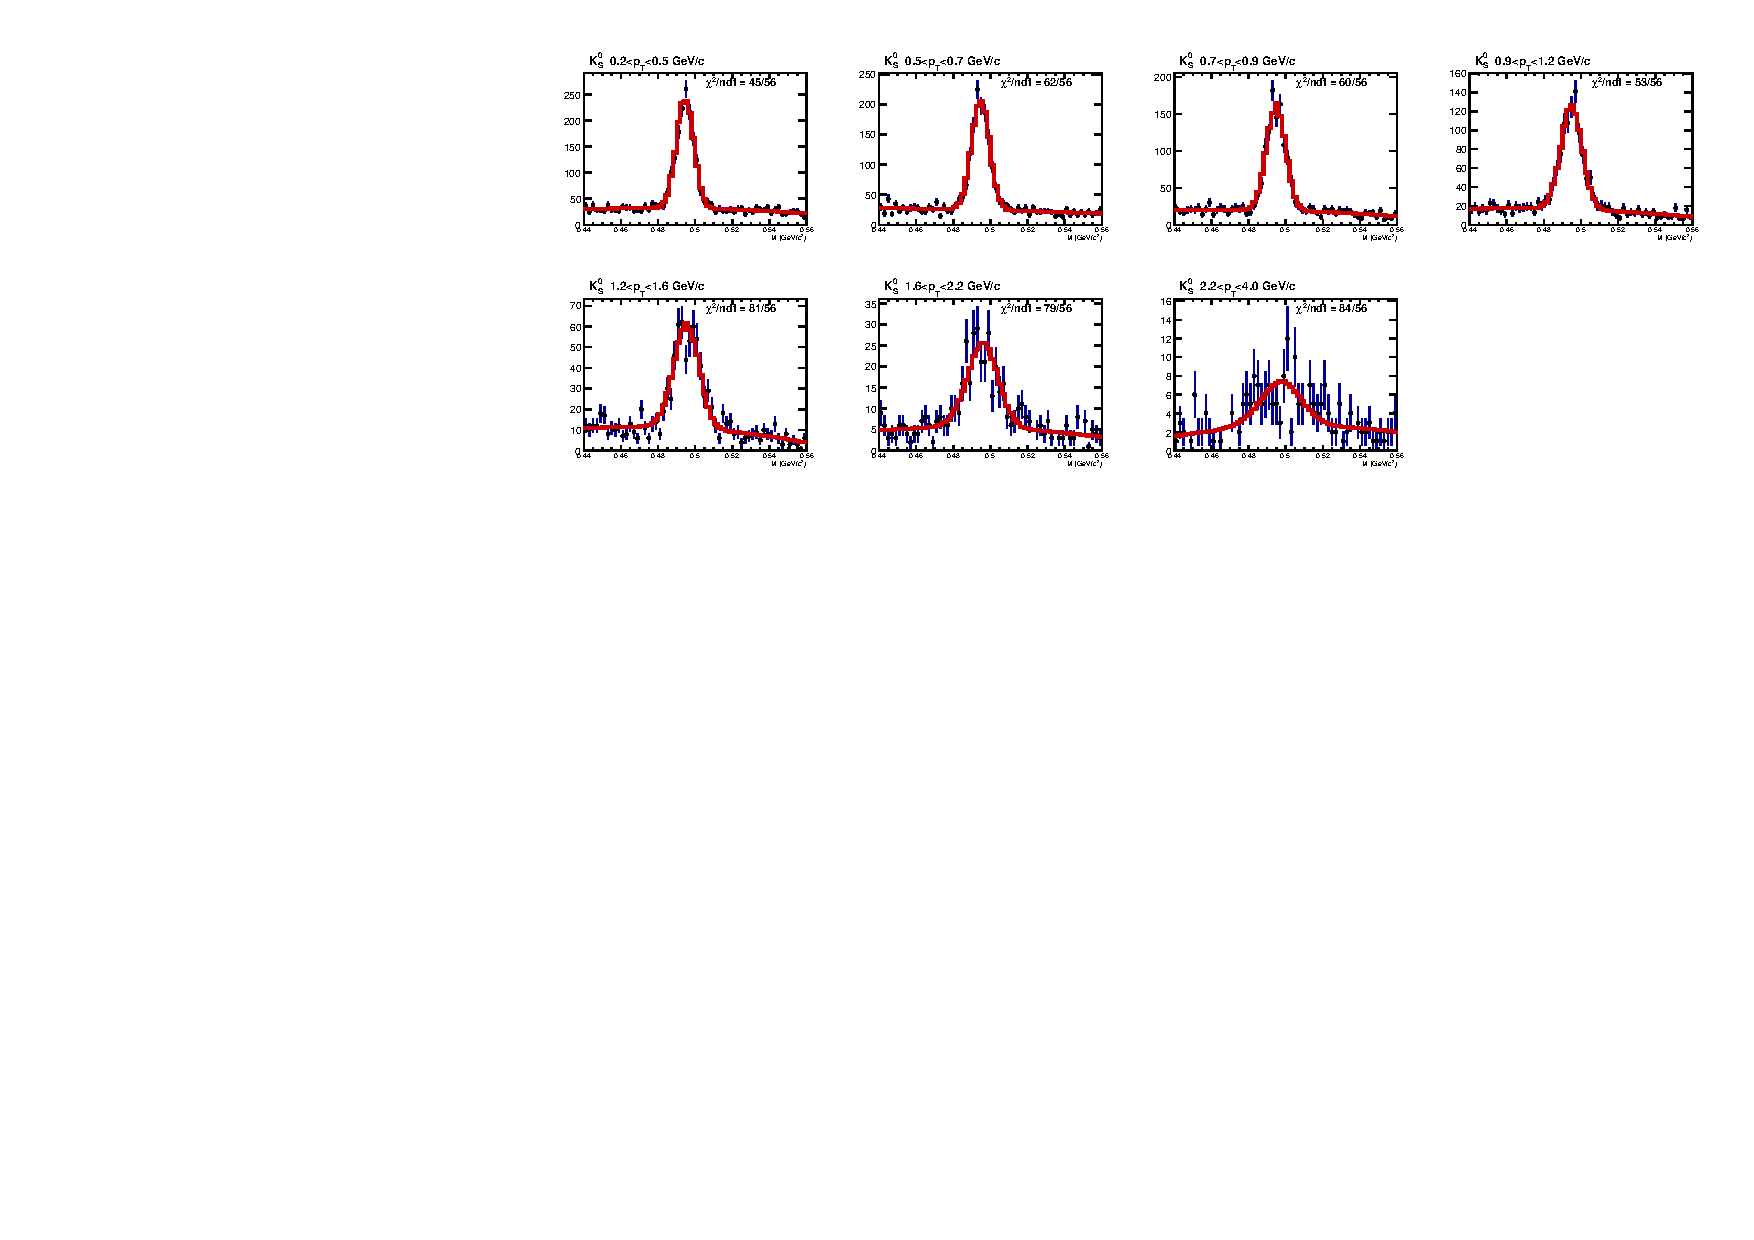
\includegraphics[width=\textwidth]{fig_mass_Ks_A_raw}
\caption{\Ks{} mass per V0-\pt{} bin, period A, recomputed without $\kappa$, with the template fit at that fit's \Ks{} best
point (red).}
\end{figure}

\begin{figure}[H]
\centering
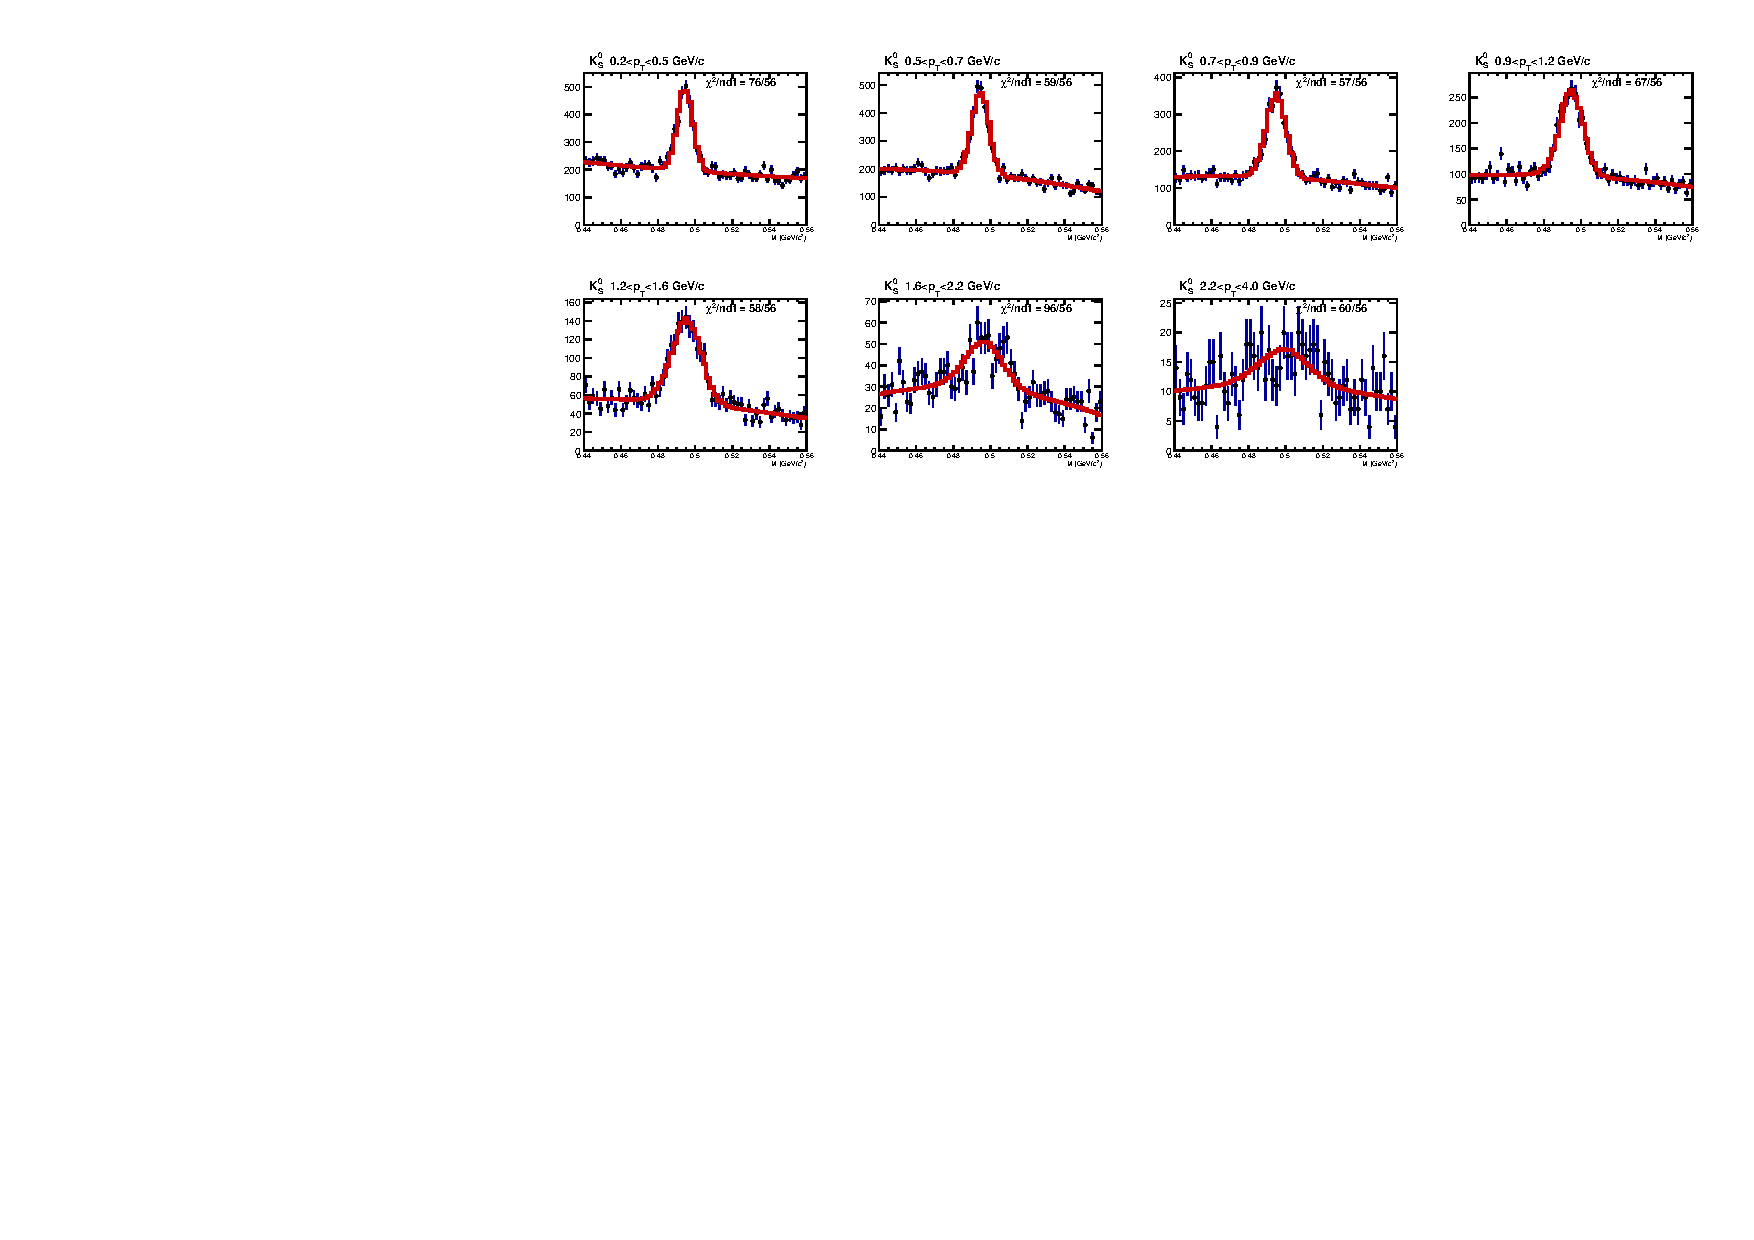
\includegraphics[width=\textwidth]{fig_mass_Ks_B_raw}
\caption{As above, period B.}
\end{figure}

\begin{figure}[H]
\centering
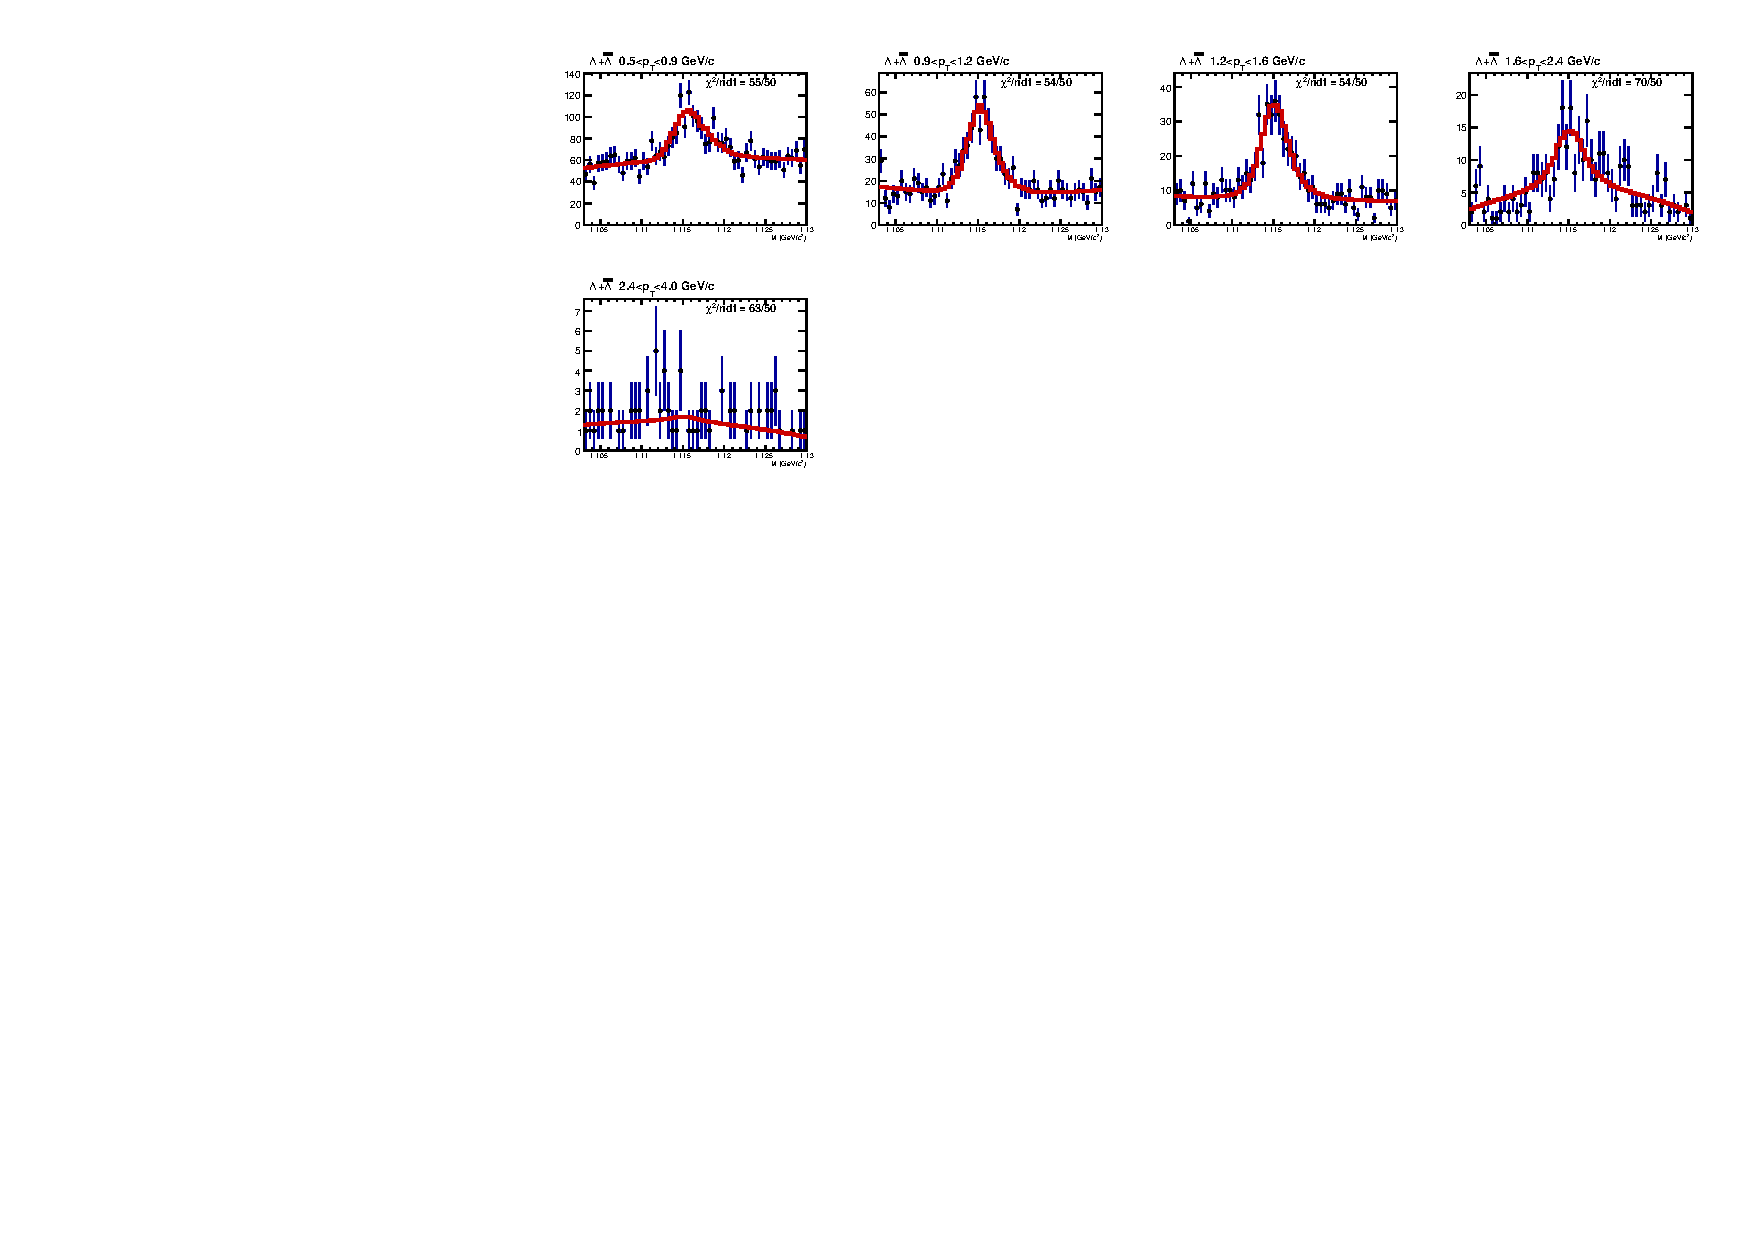
\includegraphics[width=\textwidth]{fig_mass_Lambda_A_raw}
\caption{\La+$\bar\Lambda$, period A, without $\kappa$; template at the \Ks{} best point of the same fit.}
\end{figure}

\begin{figure}[H]
\centering
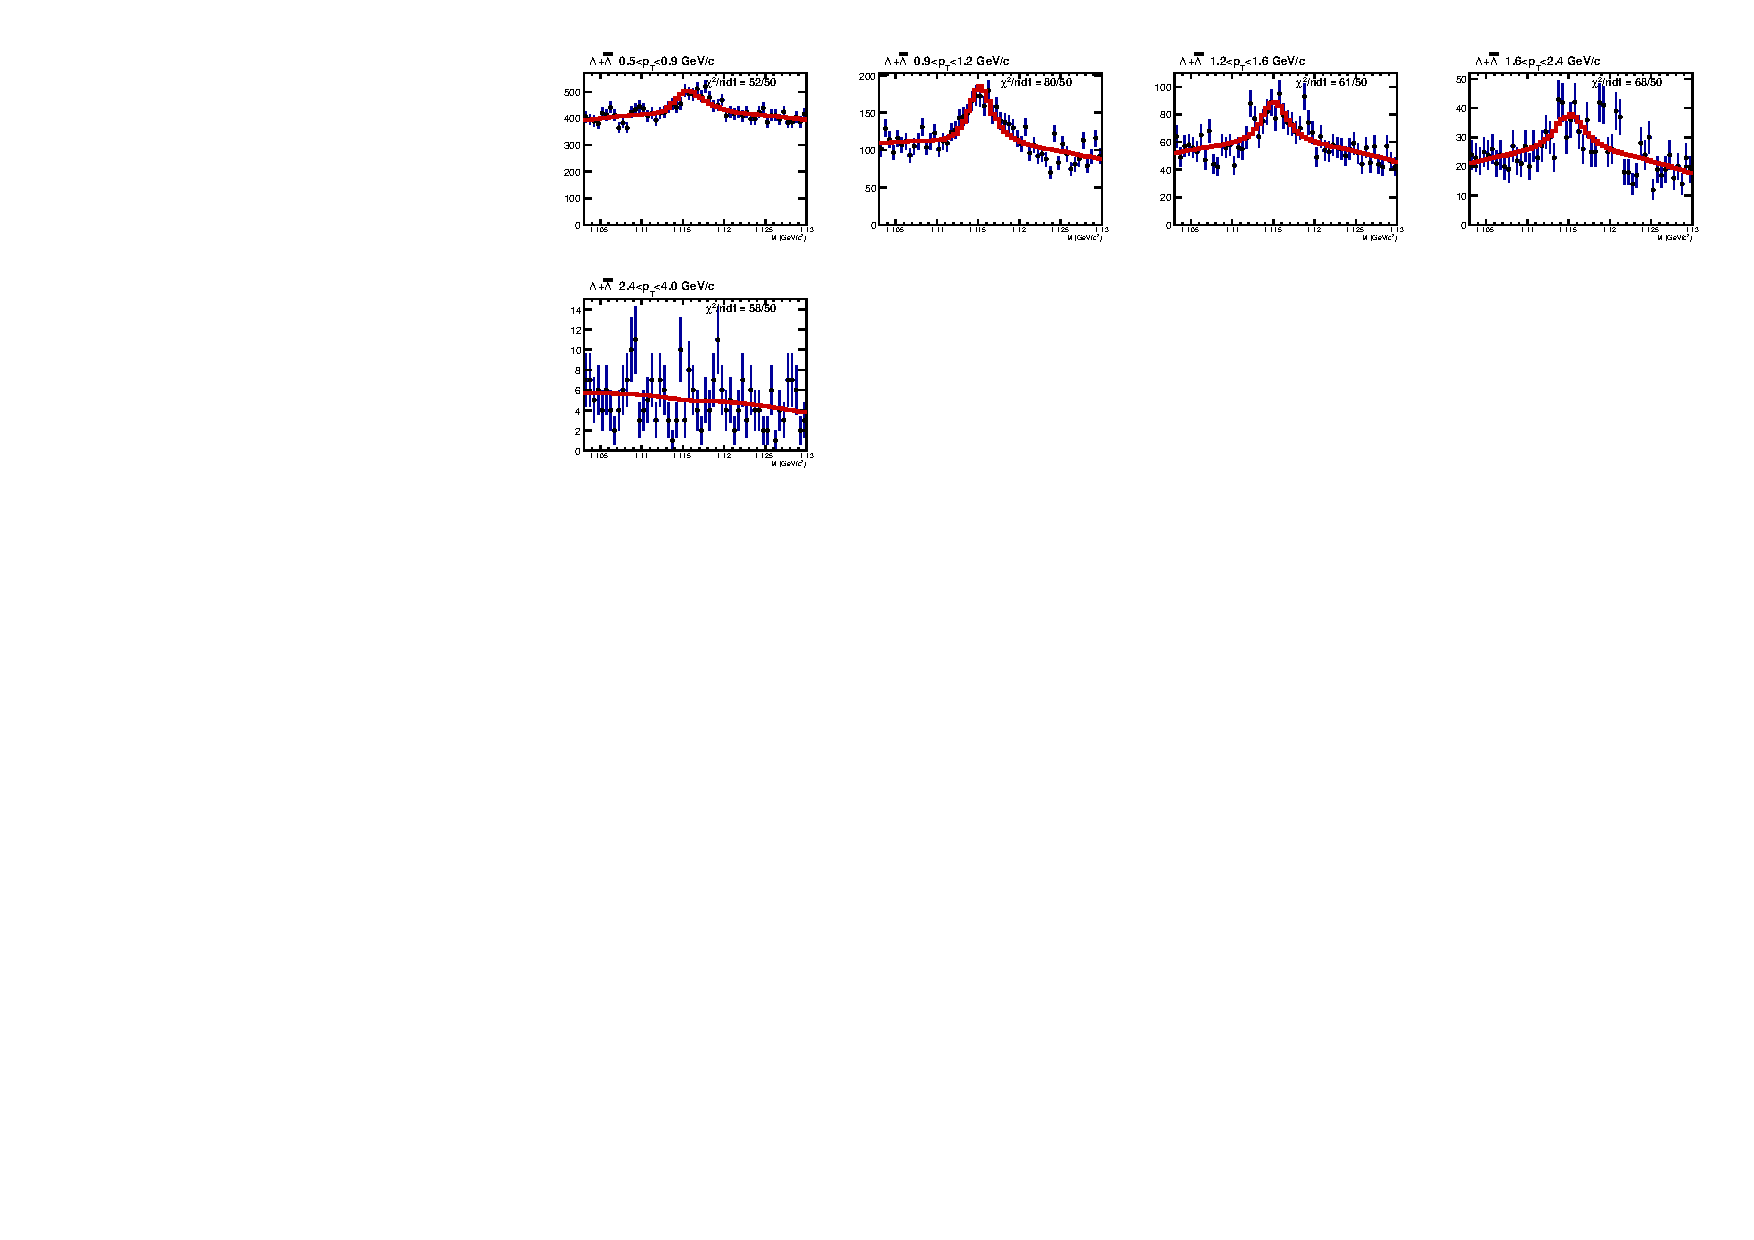
\includegraphics[width=\textwidth]{fig_mass_Lambda_B_raw}
\caption{As above, period B.}
\end{figure}


\end{document}
